%add something here
\documentclass[10pt,pdfletax,letterpaper]{sig-alternate-05-2015}

\usepackage{cite}
\usepackage{times}
\usepackage{amsmath}
\usepackage{graphicx}
\usepackage{graphics}
\usepackage{epsfig}
\usepackage{epstopdf}
\usepackage{latexsym}
\usepackage{amsfonts}
\usepackage{amssymb}
\usepackage{paralist}
\usepackage{xspace}
\usepackage{mathrsfs}
\usepackage{amssymb}
\usepackage{color}
\usepackage{algorithm}
\usepackage{algorithmic}
\usepackage{listings}
\usepackage{multirow}
\usepackage{booktabs}
\usepackage{tabularx}
\usepackage{subfigure}
\usepackage{url}
\usepackage{courier}
\usepackage{balance}

\lstset{basicstyle=\footnotesize\ttfamily,breaklines=true}
\lstset{framextopmargin=50pt}
\lstset{numbers=left}
\graphicspath{{image/}}

\setlength{\pdfpagewidth}{8.5in}
\setlength{\pdfpageheight}{11in}
%% SIGCOMM guidelines:
% Columns are 9.25 tall
% 3.33" wide with 0.33" separation
% -> 3.33"*2+0.33 = 7" -> 0.75 per left and right
% 0.75" top and 1" bottom should work out for 9.25" tall
% footskip is where the page #s go.
\usepackage[letterpaper,nohead,
	left=0.75in,right=0.75in,top=0.75in,
	footskip=0.5in,bottom=1in,
	columnsep=0.33in]{geometry}

\begin{document}

\CopyrightYear{2016}
\setcopyright{acmcopyright}
\conferenceinfo{SIGCOMM '16,}{August 22--26, 2016, Florianopolis, Brazil}
\isbn{978-1-4503-4193-6/16/08}
\acmPrice{\$15.00}
\doi{http://dx.doi.org/10.1145/2934872.2934897}


% What is going to be the name
%\title{ClickNP: A Modular Software Network Processor on Reconfigurable Hardware \vspace{-.5cm}}
\title{ClickNP: Highly Flexible and High Performance Network Processing with Reconfigurable Hardware\vspace{-0.8cm}}
\def\name{ClickNP}
\def\fullname{Click Network Processor}
\def\sysname{}

%% \vspace*{-0.1in}

\newcommand{\authornote}[1]{\raisebox{0.8ex}{$#1$}}

\numberofauthors{1}
\author{
	Bojie Li\authornote{\S\dagger} \and
	Kun Tan\authornote{\dagger} \and
	Layong (Larry) Luo\authornote{\ddagger} \and
	Yanqing Peng\authornote{\bullet\dagger} \and
	Renqian Luo\authornote{\S\dagger} \and
	Ningyi Xu\authornote{\dagger} \and
	Yongqiang Xiong\authornote{\dagger} \and
	Peng Cheng\authornote{\dagger} \and
	Enhong Chen\authornote{\S} \and
	\authornote{\dagger}Microsoft Research \quad
	\authornote{\S}USTC \quad
	\authornote{\ddagger}Microsoft \quad
	\authornote{\bullet}SJTU
	%\scalebox{0.8}{\{v-bojli, kuntan, laluo, v-reluo, v-yanpen, ningyixu, yqx, pengc\}@microsoft.com, cheneh@ustc.edu.cn}
}

\maketitle

%
% The code below should be generated by the tool at
% http://dl.acm.org/ccs.cfm
% Please copy and paste the code instead of the example below. 
%
\begin{CCSXML}
	<ccs2012>
	<concept>
	<concept_id>10003033.10003058.10003063</concept_id>
	<concept_desc>Networks~Middle boxes / network appliances</concept_desc>
	<concept_significance>500</concept_significance>
	</concept>
	<concept>
	<concept_id>10003033.10003106.10003110</concept_id>
	<concept_desc>Networks~Data center networks</concept_desc>
	<concept_significance>300</concept_significance>
	</concept>
	<concept>
	<concept_id>10010583.10010682.10010684.10010686</concept_id>
	<concept_desc>Hardware~Hardware-software codesign</concept_desc>
	<concept_significance>300</concept_significance>
	</concept>
	</ccs2012>
\end{CCSXML}

\ccsdesc[500]{Networks~Middle boxes / network appliances}
\ccsdesc[300]{Networks~Data center networks}
\ccsdesc[300]{Hardware~Hardware-software codesign}


%
% End generated code
%

%
% import the customized commands
%
\newcommand{\knote}[1]
{{$\langle${Kun: \textbf{#1}}$\rangle$}}
\newcommand{\kfnote}[1] {\footnote{\textcolor{red}{Kun: \it{#1}}}}
\newcommand{\todo}[1] {\textcolor{red}{To do: \it{#1}}}
\newcommand{\remove}[1] {{\textcolor{red}{\sout{#1}}}}
\newcommand{\add}[1] {{\textcolor{red}{\underline{#1}}}}
\newcommand{\egg}[1] {}
\newcommand{\separate}[1] {\textbf{\center ======  #1  ====== }}
\newcommand{\smalltitle}[1] {\vspace{6pt} \noindent \textbf{#1}}

\def\ie{\textit{i.e.}\xspace}
\def\etal{\textit{et al.}\xspace}
\def\etc{\textit{etc.}\xspace}
\def\eg{\textit{e.g.}\xspace}
\def\st{\xspace\textbf{s.t.}\xspace}
\def\whp{{\emph{w.h.p}}}
\def\cname{FICA \xspace}
\def\802{IEEE 802.11\xspace}
\def\arrow{$\rightarrow$}
\def\mrts{\textit{M-RTS}\xspace}
\def\mrtss{\textit{M-RTSes}\xspace}
\def\mcts{\textit{M-CTS}\xspace}
\def\mctss{\textit{M-CTSes}\xspace}
\def\approx{$\sim$}

\def\receivers{\textbf Q}
\def\capacity{{ \textbf{c}}}
\def\upperBound{{\mathcal D}}
\def\schedule{{\mathcal S}}
\def\throughput{{\cal T}}
\def\period{{\textbf Z}}

\newtheorem{theorem}{Theorem}
\newtheorem{axiom}[theorem]{Axiom}
\newtheorem{corollary}[theorem]{Corollary}
\newtheorem{definition}{Definition}
\newtheorem{lemma}[theorem]{Lemma}
\newtheorem{remark}[theorem]{Remark}

\newcommand{\prob}[1]{{\textbf{Pr}\left(#1\right)}}
\newcommand{\mcell}[2]{ \parbox[h]{#1}{ \vspace{0.5mm} #2 \vspace{0.5mm}}}

%\renewcommand\scriptsize{\@setfontsize\scriptsize\@viipt{9\p@}}
%\def\appsize{\@setsize\scriptsize{9\p@}\viipt\@viipt}

\lstdefinestyle{numbers} {numbers=left, stepnumber=1,
numberstyle=\tiny, xleftmargin=10pt, numbersep=5pt}
\lstset{language=C++}

%!TEX root=main.tex
\begin{abstract}
Highly flexible software network functions (NFs) are crucial components to 
enable multi-tenancy in the clouds.
However, software packet processing on a commodity server has limited capacity and induces high latency.
While software NFs could scale out using more servers, doing so adds significant cost.
This paper focuses on accelerating NFs with programmable hardware, \ie, FPGA, which is now a mature 
technology and inexpensive for datacenters. 
However, FPGA is predominately programmed using low-level hardware description languages (HDLs), which are hard 
to code and difficult to debug. 
More importantly, HDLs are almost inaccessible for most software programmers. 
This paper presents ClickNP, a FPGA-accelerated platform for highly flexible and high-performance NFs
with commodity servers. 
ClickNP is highly flexible as it is completely programmable using high-level C-like languages,
and exposes a modular programming abstraction that resembles Click Modular Router.
ClickNP is also high performance. 
Our prototype NFs show that they can process traffic at up to 200 million packets per second
 with ultra-low latency ($<$ 2$\mu$s).  
Compared to existing software counterparts, with FPGA, ClickNP improves throughput by 10x, while reducing latency by 10x.
To the best of our knowledge, ClickNP is the first FPGA-accelerated platform for NFs, 
written completely in high-level language and achieving 40~Gbps line rate at any packet size.
\end{abstract}

\vspace{-5pt}

%
%  Use this command to print the description
%
\printccsdesc

% We no longer use \terms command
%\terms{Theory}
\vspace{-5pt}
\keywords{Network Function Virtualization; Compiler; Reconfigurable Hardware; FPGA}


%
% section by section tex files
%
%!TEX root=main.tex
\section{Introduction}

% cloud computing
Modern multi-tenant datacenters provide shared infrastructure for hosting many different types of services 
from different customers (\ie, tenants) at a low cost.
%
To ensure security and performance isolation, each tenant is deployed in a \textit{virtualized network} environment. 
% flexible network functions
Flexible network functions (NFs) are required for datacenter operators to enforce isolation 
while simultaneously guaranteeing Service Level Agreements (SLAs). 

% host networking and software network functions
Conventional hardware-based network appliances are not flexible, 
and almost all existing cloud providers, \eg, Microsoft, Amazon and VMWare,
have been deploying software-based NFs on servers to
maximize the flexibility~\cite{albert-ons, vmware-multi-tenancy}.
%
%have implemented \textit{virtualized} network functions in hypervisor software on every server to maximize the flexibility, 
%ranging from tunning, load balancing, traffic shaping, and security (\eg, firewall)~\cite{albert-ons, vmware-multi-tenancy}. 
% note: we may need to add citation to AWS later
% limitation of software network functions
However, software NFs have two fundamental limitations -- both stem 
from the nature of software packet processing.   
% capacity
First, processing packets in software has limited capacity. 
% 
Existing software NFs usually require multiple cores to achieve 10~Gbps rate~\cite{comb, martins2014clickos}. 
But the latest network links have scaled up to 40\approx100~Gbps~\cite{mellanox-100g}. 
Although one could add more cores in a server, doing so adds significant cost,  
not only in terms of capital expense, but also more operational expense as they are burning significantly more energy. 
%
Second, processing packets in software incurs large, and highly variable latency. This latency may range 
from tens of microsecond to milliseconds~\cite{martins2014clickos, ananta, duet}. 
For many low latency applications (\eg, stock trading), this inflated latency is unacceptable. 

% hardware accelerating
To overcome the limitations of software packet processing while retaining flexibility,
recent work has proposed accelerating NFs using  
Graphics Processing Units (GPUs)~\cite{packetshader}, network processors (NPs)~\cite{cavium, netronome},
or reconfigurable hardware (\ie, Field Programmable Gate Arrays, or FPGAs)~\cite{netfpga, smartnic, rubow2010chimpp}.
% brief comparisons
Compared to GPU, FPGA is more power-efficient~\cite{fpga-vs-gpu,fpga-vs-gpu2}. 
Compared to specialized NPs, FPGA is more \textit{versatile} 
as it can be virtually reconfigured with any hardware logic for any service.
Finally, FPGAs are inexpensive and being deployed at scale in datacenters~\cite{smartnic, putnam2014reconfigurable}.

% turning directly to FPGA and its main challenge
In this work, we explore the opportunity to use FPGA to accelerate software NFs in datacenters.
The main challenge to use FPGA as an accelerator is \textit{programmability}. 
% HDL
Conventionally, FPGAs are programmed with hardware description 
languages (HDLs), such as Verilog and VHDL, which expose only low
level building blocks like gates, registers, multiplexers and clocks. 
While the programmer can manually tune the logic to achieve maximum performance,
the programming complexity is huge, resulting in low productivity and debugging
difficulties.
%
Indeed, the lack of programmability of FPGA has kept the large community 
of software programmers away from this technology for years~\cite{bacon2013fpga}. 

This paper presents \name, an FPGA-accelerated platform for 
highly flexible and high-performance NF processing 
on commodity servers. 
%
\name\ addresses the programming challenges of FPGA in three steps.
% programming model
First, \name\ provides a modular architecture, resembling the well-known 
Click model~\cite{kohler2000click}, where a complex network function is 
composed using simple, well-defined elements
\footnote{This is also where our system name, \textit{Click Network Processor}, comes from.}.  
% HLS
Second, \name\ elements are written with a high-level C-like language
 and are cross-platform. 
\name\ elements can be compiled into binaries on CPU or 
low-level hardware description language (HDL) for FPGAs, by
leveraging commercial high-level synthesis (HLS) tools~\cite{vivado, aoc, sdaccel}. 
%
% PCIE I/O, compute partitioning, and debugging
Finally, we develop a high-performance PCIE I/O channel that provides 
high-throughput and low latency communications between elements running on CPU 
and FPGA.
This PCIE I/O channel not only enables joint CPU-FPGA processing -- allowing programmers to 
partition their processing freely, but also is of great help for debugging, 
as a programmer may easily run an element in question on the host 
and use familiar software tools to diagnose. 

%While similar approaches have been tried before, \name\
%achieves more than two orders of magnitude performance improvements compared to previous work~\cite{Click2NetFPGA}.
% optimization of FPGA programming and performance
\name\ employs a set of optimization techniques to effectively utilize 
the massive parallelisms in FPGA. 
%while completely programming in high-level language. 
% divide and conque
First of all, \name\ organizes each element into a logic block in FPGA and 
connects them with first-in-first-out (FIFO) buffers.
Therefore, all these element blocks can run in full parallel.
% minimize the dependency
For each element, the processing function is carefully written to minimize the dependency among 
operations, which allows the HLS tools to generate maximum parallel logics.
Further, we develop \textit{delayed write} and \textit{memory scattering} techniques to address
the read-write dependency and pseudo-memory dependency, which cannot be resolved by existing HLS tools.
% memory
Finally, we carefully balance the operations in different stages and match their processing speed, 
so that the overall throughput of pipelines is maximized. 
% results
With all these optimizations, \name\ achieves high packet processing throughput 
up to 200 million packets per second~\footnote{The actual throughput of a \name\ NF may be bound by the Ethernet port data rate.}, with ultra-low latency ($< 2\mu$s for any packet size in most applications).
% summarize the comparison of results
This is about a 10x and 2.5x throughput gain, compared to state-of-the-art software NFs on CPU and CPU with GPU acceleration~\cite{packetshader}, 
while reducing the latency by 10x and 100x, respectively.

% implementation
We have implemented the \name\ tool-chain, which can integrate with various commercial HLS tools~\cite{vivado, aoc}. 
%including Altera OpenCL SDK, Xilinx Vivado and SDAccel. 
% elements
We have implemented about 100 common elements, 20\% of which are re-factored straightforwardly from Click. 
We use these elements to build five demonstration NFs: 
(1) a high-speed traffic capture and generator, 
(2) a firewall supporting both exact and wildcard matching, 
(3) an IPSec gateway,
(4) a Layer-4 load balancer that can handle 32 million concurrent flows, 
and (5) a pFabric scheduler~\cite{pfabric} that performs strict priority flow scheduling with 4-giga priority classes.
%
We evaluate these network functions on a testbed with 
Dell servers and Altera Stratix V FPGA boards~\cite{putnam2014reconfigurable}.
Our results show that all of these NFs can be greatly accelerated by FPGA and saturate the line rate of 40Gbps at 
any packet size with very low latency and neglectable CPU overhead.  

In summary, the contributions of this paper are: 
(1) the design and implementation of \name\ language and tool-chain; 
(2) the design and implementation of high-performance packet processing modules that are running efficiently on FPGA; 
(3) the design and evaluation of five FPGA-accelerated NFs. 
To the best of our knowledge, \name\ is the first FPGA-accelerated packet processing platform for general network functions, 
written completely in high-level language and achieving a 40~Gbps line rate.

\egg{
\smalltitle{Roadmap.} The roadmap of the paper is as follows: \S\ref{sec:background} discuss the background.
\S\ref{sec:architecture} presents the \name\ architecture and design. 
Our optimizations for FPGA is explained in \S\ref{sec:optimization}.
\S\ref{sec:impl} presents the implementation details and \name\ NFs are discribed in \S\ref{sec:application}.
We evaluate \name\ in \S\ref{sec:eval}.
Related work is discussed in \S\ref{sec:related} and 
we conclude in \S\ref{sec:conclusion} .
}

\egg{
\separate{outline}

The flow: 

Cloud services demand more and more capability. Trend in networking technologies: 40G \arrow 100G~\cite{mellanox-100g}.

Multi-tenancy cloud pushes the network edge/functions to end host~\cite{albert-ons, vmware-multi-tenancy}

Implementing network functions in software (or network function virtualization). Downsides: 1) performance (throughput and latency); and 2) cost (count \# of CPU in use). 

What are the network functions in mind?
\begin{itemize}
\item tunning
\item traffic shaping (rate limiters, load balancer)
\item security (firewall, crypto)
\item management and monitoring
\end{itemize}•


Hardware acceleration is needed. 1) GPU ~\cite{packetshader}; 2) FPGA \cite{netfpga, lockwood2007netfpga} \cite{smartnic}
We also need to mention FPGA is cost efficient~\cite{putnam2014reconfigurable}.

However, the programmability of FPGA is low. High-level Synthesizer could help. ~\cite{bacon2013fpga, feist2012vivado, auerbach2010lime, czajkowski2012opencl, Click2NetFPGA}. 
But these tools are either hard to use for software programmer, or do not have a right interface for network processing.

Why not just use OpenCL?
\begin{itemize}
\item OpenCL is originally designed to allow host program to execute a function (called kernel) on the accelerating devices.
\item With pipe object OpenCL can be used for streaming processing of packet flows, but very cumbersome, requiring manually allocating, distributing and deallocating pipe objects.
\item Code-reuse.  Hard to reuse code.
\end{itemize}•

Programming abstraction: Click model. Familiar, well modeling the packet processing flow.
Key features:
\begin{itemize}
\item elements can be executed in both CPU or FPGA. good for debugging.

\end{itemize}•


Key optimizations in FPGA:
\begin{itemize}
\item memory dependency avoidance. 1) buffer registers; 2) memory stripping; 3) dependency among processing pipelines (?) 
\item Unroll and code expansion. We need maximal iteration loop. (indeterminate, dynamically determined). 
\item Explicit pipelining (control the size of combination logic)
\end{itemize}•


Host library.

CommandHUB (hierarchical cmdhub).

PCIE I/O channels
Batching / Polling / Interrupt / sharing PCIE 

The rest of this paper is organized as follows. Section \ref{sec:background} walks through network processor architectures and programming challenges of FPGA, then propose design goals of ClickNP. Section \ref{sec:architecture} illustrates the FPGA hardware platform we work on, and provides an overview of the ClickNP toolchain. In addition to programming abstractions for writing elements in OpenCL (section \ref{sec:language}), we have also built a library of generic elements (section \ref{sec:elements}) including basic connectors, packet parsers, lookup tables, packet modifications and traffic schedulers, which can be linked as a data flow graph using Click-like syntax to perform comprehensive network functions. We evaluate our work via several high performance network applications (section \ref{sec:impl_eval}) built with ClickNP framework. Finally we discuss future works (section \ref{sec:future}) and conclude (section \ref{sec:conclusion}).
}

%!TEX root=main.tex
\section{Background}
\label{sec:background}

\subsection{FPGA architecture}
\label{subsec:fpga}
% Focus on FPGA architecture

As the name indicates, FPGA is a sea of \textit{gates}. 
The basic building block of FPGA is \textit{logic element (LE)},
which contains a Look-up Table (LUT) and a few registers. 
The LUT can be programmed to compute any combinational logic 
and registers are used to store states. 
%
Besides basic LEs, FPGA also contains Block RAMs (BRAMs) to store data, 
and Digital Signal Processing (DSP) components for complex arithmetic operations.
%
Normally, FPGAs are attached to a PC through a PCIe add-in board, which
may also contain a DRAM of multi-giga bytes and other communication
interfaces, \eg, 10G/40G Ethernet ports. 
Figure~\ref{fig:fpga} shows a logic diagram of a FPGA board.

\begin{figure}[t]
\centering
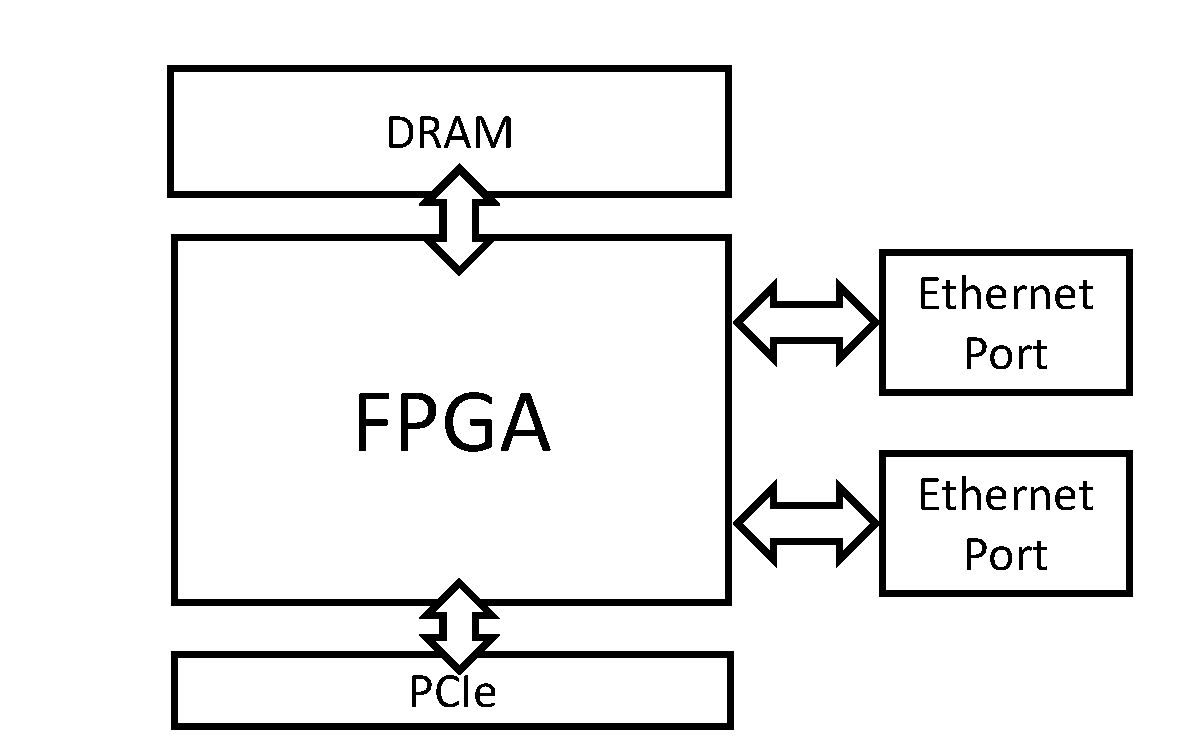
\includegraphics[width=0.3\textwidth]{fpga-board.pdf}
\vspace{-10pt}
\caption{A logic diagram of a FPGA board.}
\label{fig:fpga}
\vspace{-10pt}
\end{figure}

%
% we need to make more points here: parallelism, memory hierarchy, or code?
%

% setup the context of fpga parallelism
Compared to CPU or GPU, FPGAs usually have a much lower clock frequency
and a smaller memory bandwidth.
For example, typical clock frequency of a FPGA is about 200MHz, 
more than an order of magnitude slower than CPU (at 2\approx 3~GHz). 
Similarly, the bandwidth to a single Block memory or external DRAM of FPGA 
is usually 2\approx 10~GBps, while the memory bandwidth
is about 40~GBps of Intel XEON CPU and 100~GBps for a GPU. 
%
However, the CPU or GPU have only limited cores, which limits parallelism.
FPGAs have a massive amount of parallelism built-in. 
Modern FPGAs may have millions of LEs, hundreds K-bit registers, tens of M-bits of BRAM, 
and thousands 
of DSP blocks. In theory, each of them can work in parallel. 
Therefore, there could be thousands of parallel ``\textit{cores}'' 
running simultaneously inside a FPGA chip. 
Although the bandwidth of a single BRAM may be limited, if we access the  
thousands of BRAMs in parallel, the aggregate memory bandwidth can be multiple TBps! 
%
Therefore, to achieve high performance, a programmer
must fully utilize this massive parallelism.

% lead back to programming
Conventionally, FPGAs are programmed using HDLs like Verilog and VHDL.
These languages are too low level, hard to learn and complex to program.
As a consequence, the large community of software programmers has stayed away from FPGA for years~\cite{bacon2013fpga}. 
To ease this, many high level synthesis (HLS) 
tools/systems have been developed in
both industry and academia that try to convert a program in high level
language (predominately C) into HDLs. 
However, as we will show in the next subsection, none of them is 
suitable for network function processing, which is the focus of this work.


\subsection{Programming FPGA for NFs}

Our goal is to build a versatile, high performance network function 
platform with FPGA-acceleration. Such a platform should satisfy 
the following requirements.

\smalltitle{Flexibility.} The platform should be 
\textit{fully programmed using high-level languages.} 
Developers program with high-level abstractions and familiar tools, and
have similar programming experience as if programming on a multi-core processor.
We believe this is a necessary condition for FPGA to be accessible to
most software programmers.

\smalltitle{Modularized.} We should support a \textit{modular architecture}
for packet processing. Previous experiences on virtualized NFs
have demonstrated that a right modular architecture can well capture many common 
functionalities in packet processing~\cite{kohler2000click,martins2014clickos},
making them easy to reuse in various NFs.

\smalltitle{High performance and low latency.} NFs in datacenters
should handle a large amount of packets flowing at the line-rates of 40/100~Gbps
with ultra-low latency. Previous work has shown~\cite{rollback-mb} that even a few
hundred microseconds of latency added by NFs would have 
negative impacts on service experience.

\smalltitle{Support joint CPU/FPGA packet processing.} We'd say FPGA is no panacea. 
As inferred from the FPGA architecture discussed earlier in \S\ref{subsec:fpga}, not all tasks are 
suitable for FPGA. For example, algorithms that are naturally sequential and
processing that has very large memory footprint with low locality, should process  
better in CPU.
Additionally, FPGA has a strict area constraint. 
That means you cannot fit an arbitrarily large logic into a chip.
Dynamically swapping FPGA configurations without data plane interruption
is very difficult, as the reconfiguration time may take
seconds to minutes, depending on the FPGA's size.
%
Therefore, we should support fine-grained processing 
separation between CPU and FPGA. This requires high-performance communication 
between CPU and FPGA.


No of existing high level programming tools for FPGA satisfy all aforementioned requirements.
% HLS
Most HLS tools, \eg, Vivado HLS~\cite{vivado}, are only auxiliary tools 
for HDL tool chains. 
Instead of directly compiling a program into FPGA images, these tools generate only hardware 
modules, \ie, IP cores, which must be manually embedded in a HDL project and connected to other HDL modules
-- a mission impossible for most software programmers. 

% OpenCL
Altera OpenCL, however, may directly compile an OpenCL program to FPGA~\cite{aoc}. 
However, the OpenCL programming model is directly derived from GPU programming and 
is not modularized for packet processing. 
%
Further, OpenCL does not support joint packet processing between CPU and FPGA very well:
%
First, communication between a host program and a kernel in FPGA must always go through the onboard DDR memory. This adds non-trivial latency
and also causes the on-board memory a bottleneck.
%
Second, OpenCL kernel functions are \textit{called} from the host program. 
Before a kernel terminates, the host program cannot control the kernel behavior, \eg setting new parameters, nor reading any kernel state. 
But NFs face a continuous stream of packets and should be always running.

Click2NetFPGA~\cite{Click2NetFPGA} provides a modular architecture by 
directly compiling a Click modular router~\cite{kohler2000click} program into FPGA.
%
However, the performance of \cite{Click2NetFPGA} is much lower (two orders of magnitude) than what we report in this paper, as there are several bottlenecks in their system design (\eg, memory and packet I/O) and they also miss 
several important
optimizations to ensure fully pipelined processing (as discussed in~\S\ref{sec:optimization}). 
Additionally, \cite{Click2NetFPGA} does not support FPGA/CPU joint processing and thus unable to update configuration or read states while data plane is running.


In the following, we will present \name, a novel FPGA-accelerated 
network function platform that satisfies all aforementioned four requirements.


\egg{
Today's data centers rely on a wide range of network functions to implement network virtualization, ensure security (e.g. firewalls and intrusion detection/prevention systems), perform measurements and improve performance (e.g. traffic scheduling). As data centers are moving towards 40 Gbps bandwidth at end hosts, where the line-rate is 60 M packets per second for minimum-sized packets, higher throughput requirement is imposed upon network processors. Furthermore, as data center services are evolving rapidly, programmability becomes indispensable for network processors. However, existing network processors has a large mismatch to the performance and programmability requirements.

\subsection{Architectures for Network Processors}

Network processors based on general-purpose CPUs such as ClickOS \cite{martins2014clickos} enjoy good programmablity, modularity and composabilty, but the packet forwarding performance of a single core could not keep up with 10 Gbps line rate for minimum-sized packets, even before any network function is plugged in. Because CPU instructions are executed one-by-one and have low parallelism, packet processing performance would drop further as more network functions are added. If a CPU-based network processor is added bump-in-the-wire, there will be 10s of microseconds additional end-to-end latency \cite{martins2014clickos} which is one magnitude higher than the switching fabric. In network virtualization scenario, if packet encapsulation and decapsulation is done at end hosts, as in the case of virtual switch, NIC offloading mechanisms including Large Send Offload (LSO) and Large Receive Offload (LRO) have to be disabled, which has a huge impact on TCP performance \cite{yoshino2008performance}.

ASICs are known to be high-performance, but the network functions are fixed. Commodity switching ASICs typically have a pipeline of network functions \cite{broadcomethernet}, where each function can be configured via registers and a match table based on TCAM or memory. Some ASICs provide flexible OpenFlow-like match-action tables \cite{broadcomopenflow}, but the packet parser is fixed (we could not support new packet header and shim layer formats), actions are not extensible and the order of network functions in the pipeline is not reconfigurable.

GPUs are widely used as co-processors for computing-intensive tasks, but its SIMD (Single-Instruction Multiple-Data) programming model does not fit network processing, where different types of packets may take various execution flows. The high power consumption, high latency of batch processing and inability to receive and send network packets without CPU intervention are also factors that render GPU-based network processor infeasible in data centers.

Fortunately, reconfigurable hardware is an architecture that provides both programmability, high performance and power efficiency for certain workloads. FPGA (field programmable gate arrays) is the most prominent example of reconfigurable hardware. FPGAs can implement arbitrary logic function and utilize distributed on-chip registers and SRAM to exploit bit-level and task-level parallelism, therefore stream processing pipelines would not ``hit the memory wall'' as in Von Neumann architecture \cite{bacon2013fpga}. FPGA has shown potential in accelerating many workloads in cloud \cite{putnam2014reconfigurable}. Moreover, Moore's law is still working in FPGA industry, because the fabrication technology of FPGA is currently several generations behind the CPU industry [citation required].

\subsection{FPGA Programming Challenge}

Despite FPGA's potential in network processing, the programmablity of FPGA is traditionally provided by hardware description languages (HDL) such as Verilog, which requires hardware knowledge and are much harder to program and debug than higher-level languages such as C/C++. Thus, existing FPGA-based network processors such as NetFPGA \cite{lockwood2007netfpga} are hard to program for software engineers.

Many works, e.g. OpenFlow \cite{mckeown2008openflow}, P4 \cite{bosshart2014p4} and SDNet \cite{xilinxsdnet}, provides the programmability by abstracting a set of primitives in network processing and defining a high-level programming language to compose the primitives. This direction has proved effective, but the programmability is limited to a set of pre-defined actions, which could not keep pace with rapid development of data center network functions. Our work strive to make the primitives extensible for software engineers.

Fortunately, several frameworks have been proposed to provide abstractions for generic FPGA programming. Examples of such works include Xilinx Vivado HLS (High Level Synthesis) \cite{feist2012vivado} based on C/C++, Altera SDK for OpenCL \cite{czajkowski2012opencl} based on C-like OpenCL and IBM Lime \cite{auerbach2010lime} based on Java.

However, FPGA has a completely different architecture than general-purpose CPUs. For software programmers that bear Von Neumann model in mind, the compilers may generate surprisingly poor hardware logic for reasonable code in high-level language. For example, Click2NetFPGA \cite{Click2NetFPGA} uses LLVM and HLS tools to compile optimized Click C++ code into HDL, but the resulting FPGA-based router can only process 178 K pps (packets per second) for 98B packets, and 215 Mbps for large packets, which is 30 -- 50x slower than a CPU core in ClickOS \cite{martins2014clickos}. The bottleneck for small packets is the IP header checking stage \cite{Click2NetFPGA} because this stage is not fully pipelined; the bottleneck for large packets is the byte-wide shared memory \cite{Click2NetFPGA}, indicating a shared-memory design suitable for Von Neumann model would yield poor performance on FPGA.

FPGA has millions of logic gates with 10x slower clock rate than CPU, thousands of distributed fast SRAMs each with only KB capacity, and a large DRAM with 10x lower throughput than DRAMs in CPU architecture. Consequently, exploiting both spatial and temporal parallelism is crucial to unleashing the performance of FPGA. In network stream processing, most operations are independent of each other and therefore can be either parallelized (spatial) or pipelined (temporal), so that each stage of the pipeline can process different packets in parallel.

\subsection{Design Goals}
\label{subsec:designgoals}

We highlight several design goals for our ClickNP framework to enable software engineers to write efficient network applications.

\smalltitle{Modularity.} Modularity is one key feature that improves parallelism, since modules do not have shared state and can run in parallel by nature. Borrowing the concepts from Click modular router \cite{kohler2000click}, \textit{elements} are basic building blocks of network functions. Elements run asynchronously and are connected via uni-directional \textit{channels}. The network processing pipeline is a data flow graph of elements and channels, starting from Ethernet receivers and ending at Ethernet transmitters.

\smalltitle{Line-rate throughput.} To allow efficient processing of packet content, an Ethernet packet is split into 32-byte \textit{flits} before feeding into elements. In the worst case, when 69-byte packets are received back-to-back, the line rate would be 40G / 8 / (69+20) = 56.18 Mpps, which splits into 56.18M * 3 = 168.54M flits. Every clock cycle an element reads at most one flit and outputs zero or one flit. This means any FPGA pipeline with clock frequency lower than 168.54 MHz would not be able to achieve line rate. If we waste a cycle between every two packets, the minimum clock frequency would be 224.72 MHz. However, on Stratix V FPGA platform \cite{stratix2012device}, non-trivial hardware logic that accesses registers and local memory can hardly run higher than 200 MHz. Therefore no idle cycles are allowed in elements processing packet content. First, the framework should provide abstractions for programmers to develop fully pipelined network functions. Second, as full compilation of a FPGA program may take hours, the framework should give performance warnings in an early compilation stage if the code cannot be fully pipelined.

\smalltitle{Code reuse.} Many network applications share a common set of elements, for example packet parser, lookup tables and packet modifications. Code of these elements should be reusable and elements should be composable. Software engineers should be able to write many network applications simply by connecting elements in the library.

\smalltitle{Debugging support.} First, as HDL (e.g. Verilog) simulation and debugging is both time consuming and requires extensive hardware knowledge, the framework should be able to compile OpenCL-based ClickNP programs to native x86 code for emulation, and provide traffic generators and receivers to test functionality. Second, as CPU is neither capable of sending or receiving packets at 60 Mpps, we need a FPGA-based network benchmark suite to perform stress testing on the network processor.

\smalltitle{Separation of control plane and data plane.} On one hand, our throughput requirement requires most network packets to be processed through the reconfigurable hardware without any CPU intervention. On the other hand, SDN and NFV applications are usually complicated and have external dependencies. Therefore a clear interface between the control plane and the data plane is mandatory, where data plane programs are written within ClickNP framework and target massive parallelism, and control plane programs need only slight modifications to call our host library and perform on-the-fly reconfigurations.

\smalltitle{Host communication.} Network processors require low-latency and high-throughput interactions with the host machine. In SDN and NFV applications, FPGA needs to send unknown packets to the controller and request a new forwarding rule to be inserted into FPGA. The round-trip time should be as low as possible to reduce end-to-end flow establish time. In packet replay and capture applications, FPGA needs to receive or send Gigabytes of packets from or to the host machine without using the network adapter.

We design ClickNP to meet the above design goals with Catapult FPGA \cite{putnam2014reconfigurable} and Altera OpenCL \cite{singh2011implementing}. In the next section, we will describe the FPGA and OpenCL components, and how we build a toolchain that abstracts away hardware specific details.
}

\egg{
\subsection{FPGA in datacenter}

Conventionally, datacenter operators largely relied on the performance improvements in general-purpose servers
to improve the operation efficiency. This performance improvement rate of servers 
has considerably slowed down recently due to the power limitations~\cite{putnam2014reconfigurable, more-citation}.
This has motivated the adoption of \textit{accelerator} that can be specialized to certain workloads to get efficiency gains.
However, the non-programmable ASIC-based accelerators are undesirable for datacenters due to following two reasons:
Firstly, datacenter operators prefers homogeneous server configurations to minimize the management overhead and also provide
a consistent platform that applications can rely on.
Secondly, services in datacenters evolve extremely rapidly. Waiting for the long release cycle of ASIC chips is undesirable.
%
Therefore, it requires a flexible accelerator that can potentially speed up many applications.
%
GPU and FPGA are two predominate technologies that satisfy this requirement.

% comparison between GPU and FPGA
% power efficiency
Compared with GPU, FPGA is more power efficient. For example, the latest NIVDIA xxx consumes xxx W power, while a high-end
Altera Stratix V consumes xxx W power ( J per op?) \knote{need a citation}. 
% versatile 
Further, FPGA is more versatile. While GPU is mainly designed to achieve \textit{data parallelism} with SPMD (single program, multiple data), 
FPGA can easily achieve both data parallelism and \textit{task parallelism} as different block of LEs can be independently configured to
implement different processing.  
% I/O
Finally, FPGA supports various I/O interface. Normally, GPU can only communicate with PC memory through PCIE bus. 
But FPGA can input or output data from many interfaces like network ports, and is more suitable for processing these 
I/O streams. 

FPGA is a mature technology and becomes inexpensive. A large scale deployment of FPGA in Microsoft datacenter shows 
that a high-end FPGA board increases the total cost of ownership (TCO) of a server by less than 30\%, but can double 
the Bing search efficiency~\cite{putnam2014reconfigurable}.
%
In this paper, we focus on using FPGA to accelerate network functions that are essential to our datacenter networks.
}

\egg{
\smalltitle{inexpensive}

Why I need this as background:
\begin{itemize}
\item Price issue?
\item Power?
\item Transition to FPGA for network functions?
\end{itemize}
}

%!TEX root=main.tex
\section{Architecture}
\label{sec:architecture}

\subsection{System architecture}
\label{subsec:sysarch}

\begin{figure}
\centering
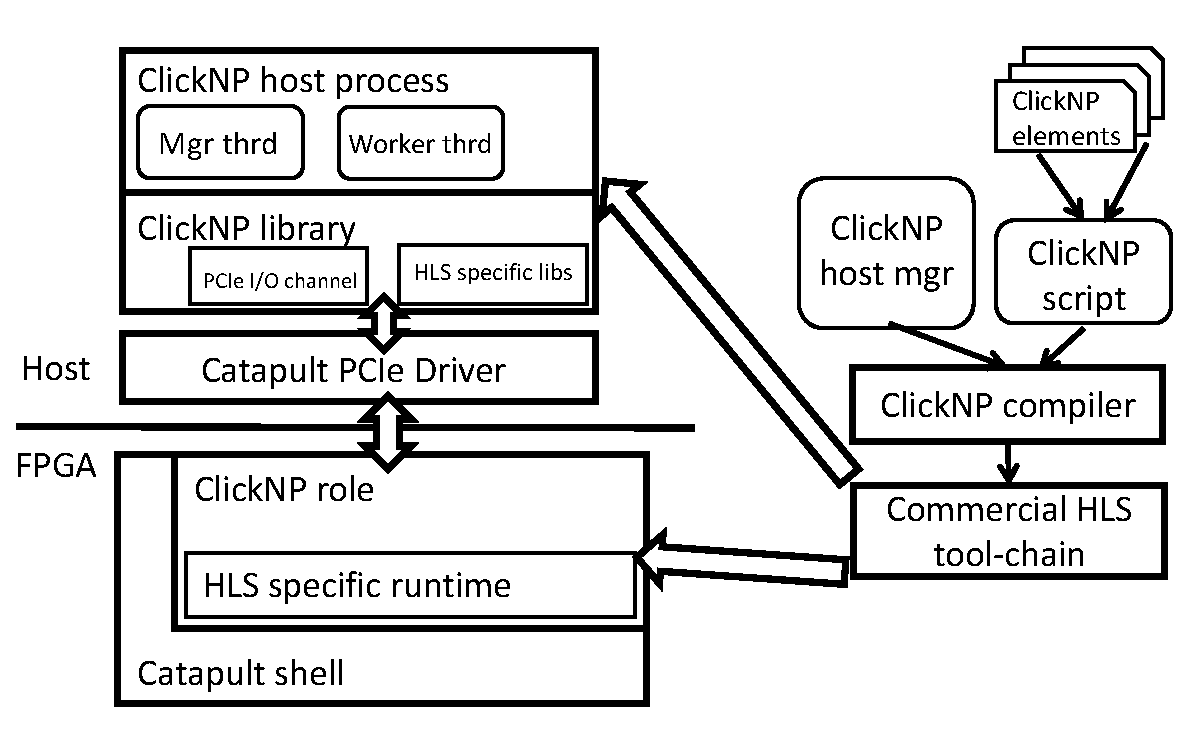
\includegraphics[width=.5\textwidth]{clicknp-arch.pdf}
\vspace{-30pt}
\caption{The architecture of ClickNP.}
\label{fig:clicknp}
\vspace{-10pt}
\end{figure}

Figure~\ref{fig:clicknp} shows the architecture of \name.
\name\ builds on the Catapult Shell architecture~\cite{putnam2014reconfigurable}.
The \textit{shell} contains many reusable bits of logic that are common for all applications 
and abstracts them into a set of well-defined interfaces,
\eg, PCIe, Direct Memory Access (DMA), DRAM Memory Manage Unit (MMU), 
and Ethernet MAC.
%
The \name\ FPGA program is synthesized as a Catapult \textit{role}.
%
However, since \name\ relies on commodity HLS tool-chains to generate FPGA HDL, 
and different tools may generate their own (and different) interfaces for the resources managed by the shell, 
we need a shim layer, called \textit{HLS-specific runtime}, to perform
translations between HLS specific interfaces to the shell interfaces. 

A \name\ host process communicates with the \name\ role through the \name\ library,
which further relies on the services in Catapult PCIe driver 
to interact with FPGA hardware.
The \name\ library implements two important functions: 
(1) It exposes a PCIe channel API to achieve high-speed and low latency communications 
between the \name\ host process and the role; 
(2) It calls several HLS specific libraries to pass initial parameters to
the modules in the role, as well as control the start/stop/reset of these 
modules.
%
The \name\ host process has one manager thread and zero or multiple 
worker threads.
%
The manager thread loads the FPGA image into the hardware, starts worker threads, 
initializes \name\ elements in both FPGA and CPU based on the configuration, 
and controls their behaviors by sending \textit{signals} to elements 
at runtime. 
%
Each worker thread may process one or more modules if they are assigned to CPU.

\subsection{\name\ programming}

\subsubsection{Abstraction}

\name\ provides a modular architecture and the basic processing module is called an \textit{element}.
A \name\ element has the following properties: 
\begin{itemize}
\item Local states. Each element can define a set of local variables that are only accessible inside the element. 
\item Input and output ports. An element can have any number of input or output ports. 
\item Handler functions. An element has three handler functions: (1) an initialization handler, which is called once when the
element starts, (2) a processing handler, which is continuously called to check input ports and process available data,
and (3) a signal handler, which receives and processes the commands (\textit{signals}) from the manager thread in the host program.
\end{itemize}

%\vspace{-6pt}
An output port of an element can connect to an input port of another element through a \textit{channel}, as shown in Figure~\ref{fig:element}(a).
In \name, a channel is basically a FIFO buffer that is written to one end and read from the other end.
The data unit of the read/write operations to a channel is called \textit{flit}, which has a fixed size of 64 bytes.
The format of a flit is shown in Figure~\ref{fig:element}(b). Each flit contains a header for meta-data and a payload of 32 bytes.
A large piece of data, \eg, a full-sized packet, is broken into multiple flits, when flowing among \name\ elements.
%Currently, we choose 32-byte data bus size, and therefor to allow up to 51.2Gbps throughput under 200MHz clock.}
The first flit is marked with \textbf{sop} (start of packet), and the last flit is marked with \textbf{eop} (end of packet). 
If the size of the data piece is not 32, the \textbf{pad} field of the last flit indicates how many bytes have been padded to the payload. 
%Reserved field in a flit is optimized out by HDL synthesis tools.
% why flit
We note that breaking large data into flits not only reduces latency, but also potentially increases parallelism as
different flits of a packet may be processed at different elements simultaneously.
%
Finally, to fulfill a network function, multiple \name\ elements can be interconnected to form a directed processing graph, which 
is called a \name\ \textit{configuration}. 

Clearly, the \name\ programming abstraction largely resembles Click software router~\cite{kohler2000click}. 
However, there are three fundamental differences which make \name\ more suitable
for FPGA implementation:
(1) In Click, edges between elements are C++ function calls and a \textit{queue} element is required to store packets.
However, in \name, an edge actually represents a FIFO buffer that can hold actual data. Additionally, \name\ channels break the data dependency among elements and allow them to run in parallel. 
%	FIFO also leverages \textit{pipe} abstraction in OpenCL for efficient hardware generation.
(2) Unlike Click, where each input/output port can be either \textit{push or pull}, 
\name\ has unified these operations: An element can only \textit{write (push)}  to any output port, while \textit{read (pull)} can do so from any input port.
%This is a more flexible model and allows elements to be reused in both ingress and egress pipeline.
(3) While Click allows an element to directly call methods of another element (via flow-based router context), in \name,
the coordination among elements is \textit{message-based}, \eg, a requester sends a request message to a responder and gets a response via another message.
%
Message-based coordination allows more parallelism and is more efficient in FPGA compared to coordination through shared memory, where accessing a shared memory location has to be serialized and would become a bottleneck.

\begin{figure}
\centering
\begin{tabular}{c}
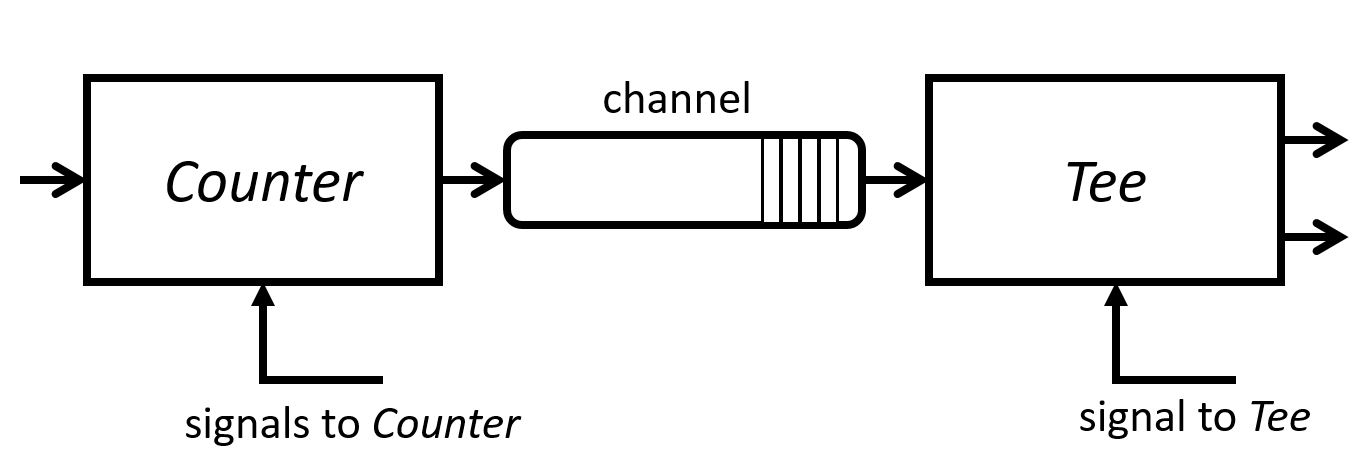
\includegraphics[width=.4\textwidth]{element.jpg} \vspace{-6pt} \\
(a)\\
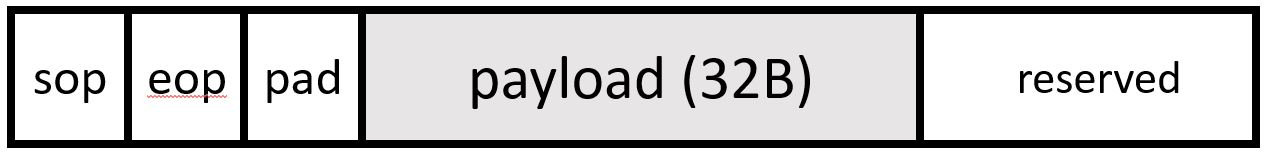
\includegraphics[width=.35\textwidth]{flit.jpg} \\
(b) \\
\end{tabular}
\vspace{-10pt}
\caption{(a) Two \name\ elements are connected through a channel. (b) The format of a flit. }
\label{fig:element}
\vspace{-17pt}
\end{figure}

\subsubsection{Language}

\name\ elements are alike objects in an object-oriented language, and can be defined using such languages, \ie, C++.
Unfortunately, many existing HLS tools support only C. 
To leverage the commercial HLS tools, we could write a compiler that converts a object-oriented language, \eg C++, to C.
But this effort is non-trivial.
In this work, we take an alternative path to extend C language to support element declaration.
Figure~\ref{fig:lang}(a) shows a code snippet of element \textit{Counter}, which simply counts how many packets have
passed. An element is defined by \textbf{.element} keyword, followed by the element name and the number of input/output ports.
The keyword \textbf{.state} defines the state variables of the element, and \textbf{.init}, \textbf{.handler}, and \textbf{.signal}
specify the initialization, processing, and signal handler functions of the element.
A set of built-in functions are implemented to operate on the input and output ports, as summarized in Table~\ref{tab:built-in}.

Similar to Click, \name\ also uses a simple script to specify a configuration of a network function. The configuration has
two parts: \textit{declarations} and \textit{connections}, following the similar syntax of Click language~\cite{kohler2000click}.
One thing worth noting is that in \name\, we can use a keyword \textbf{host} to annotate an element, which will cause 
the element to be compiled into CPU binary and executed on CPU.

\begin{table}
\vspace{-10pt}
\centering
\caption{Built-in operations on \name\ channels.}
\label{tab:built-in}
\small
\begin{tabular}{p{.2\textwidth}|p{4cm} }
\toprule \\
uint get\_input\_port() & Get bitmap of all input ports with available data. \\
\midrule
bool test\_input\_port(uint id) & Test the input port indicated by id. \\
\midrule
flit read\_input\_port(uint id) & Read the input port indicated by id. \\
\midrule
flit peek\_input\_port(uint id) & Peek input data from the port indicated by id. \\
\midrule
void set\_output\_port(uint id, flit x) & Set a flit to the output port. The flit is written to the channel when the handler returns.\\
\midrule
ClSignal read\_signal() & Read a signal from signal port.\\
\midrule
void set\_signal(ClSignal p) & Set an output signal on signal port.\\
\midrule
return (uint bitmap) & Return value of \textbf{.handler} specifies a bitmap of input port(s) to be read on next iteration. \\
\bottomrule
\end{tabular}
\vspace{-10pt}
\end{table}

\begin{figure}[t!]
\scriptsize \lstset{style=numbers}

\lstset{ emph={%
 element, init, state, handler, signal,include
}, emphstyle={\bfseries .},
morekeywords={get_input_port,read_input_port,from_tor, to_tor, set_output_port, host, set_signal} 
}
\centering
\begin{tabular}{c}

\begin{lstlisting}
element Count <1, 1> {
  state{
    ulong count;
  }
  init{
    count = 0;
  }
  handler{
    if (get_input_port() != PORT_1) {
      return (PORT_1); 
    }
    flit x;
    x = read_input_port(PORT_1);
    if (x.fd.sop) count = count + 1;
    set_output_port(PORT_1, x);
   
    return (PORT_1);
  }
  signal{
    ClSignal p;
    p.Sig.LParam[0] = count;
    set_signal(p);
  }
}
\end{lstlisting} \vspace{3pt} \\
{\normalsize \centering (a)} \vspace{3pt} \\
\begin{lstlisting}
Count :: cnt @ 
Tee :: tee 
host PktLogger :: logger

from_tor -> cnt -> tee [1] -> to_tor
tee [2] -> logger
\end{lstlisting} \vspace{3pt} \\
{\normalsize \centering (b)} 
\end{tabular}
\caption{\name\ language to write elements and specify configurations. An element annotated with \textbf{host} keyword is compiled and executed on the CPU. An element annotated with ``@'' is required to receive control signals from the manager thread. 
\textbf{``From\_tor''} and \textbf{``to\_tor''} are two built-in elements that represent input and output of an Ethernet port on FPGA. The return value of the handler function specifies
a bit-mask of input ports that will be checked in next round.}
\label{fig:lang}
\vspace{-10pt}
\end{figure}

\subsubsection{\name\ tool-chain}
\label{subsec:toolchain}
The \name\ tool-chain contains a \name\ compiler as the front-end, and a C/C++ compiler (\eg, Visual Studio or GCC) and an HLS tool 
(\eg, Altera OpenCL SDK or Xilinx Vivado HLS) as the back-end.
% Overview of ClickNP programming process
As shown in Figure~\ref{fig:clicknp}, to write a \name\ program, a developer needs to divide her code into three parts:
% very similar to the Click Modular Router~\cite{kohler2000click}:
(1) A set of elements, each of which implements a conceptually simple operation,
(2) A configuration file that specifies the connectivity among these elements,
and (3) A host manager that initialize each element and control their behavior during the runtime, \eg, according to the input of administrators.
%
These three parts of source code are fed into the \name\ compiler and translated 
into intermediate source files for both host program and FPGA program. 
The host program can be directly compiled by a normal C/C++ compiler, while the FPGA program is synthesized using commercial HLS tools.
%
Existing commercial HLS tools can determine a maximum clock frequency of 
each element through timing analysis. 
Then, the clock of a \name\ processing graph is constrained by the slowest element in the graph.
%
Additionally, HLS tools may also generate an optimization report which shows the 
dependency among the operations in an element. An element is \textit{fully pipelined}
if all dependency is resolved and the element achieves the optimal throughput by 
processing one flit in every clock cycle.

\egg{
Our ClickNP architecture is built on state-of-the-art data center reconfigurable hardware (Catapult FPGA \cite{putnam2014reconfigurable}) and FPGA programming framework (Altera OpenCL \cite{singh2011implementing}).

\subsection{Catapult FPGA}

Catapult \cite{putnam2014reconfigurable} is a reconfigurable hardware designed for offloading feature extraction, feature computation and scoring in search engine ranking. We modify the hardware to incorporate two on-board 40 GE MACs, so the FPGA can receive and send network packets via the two 40 GE ports without CPU intervention.

\begin{figure}[!t]
	\center
	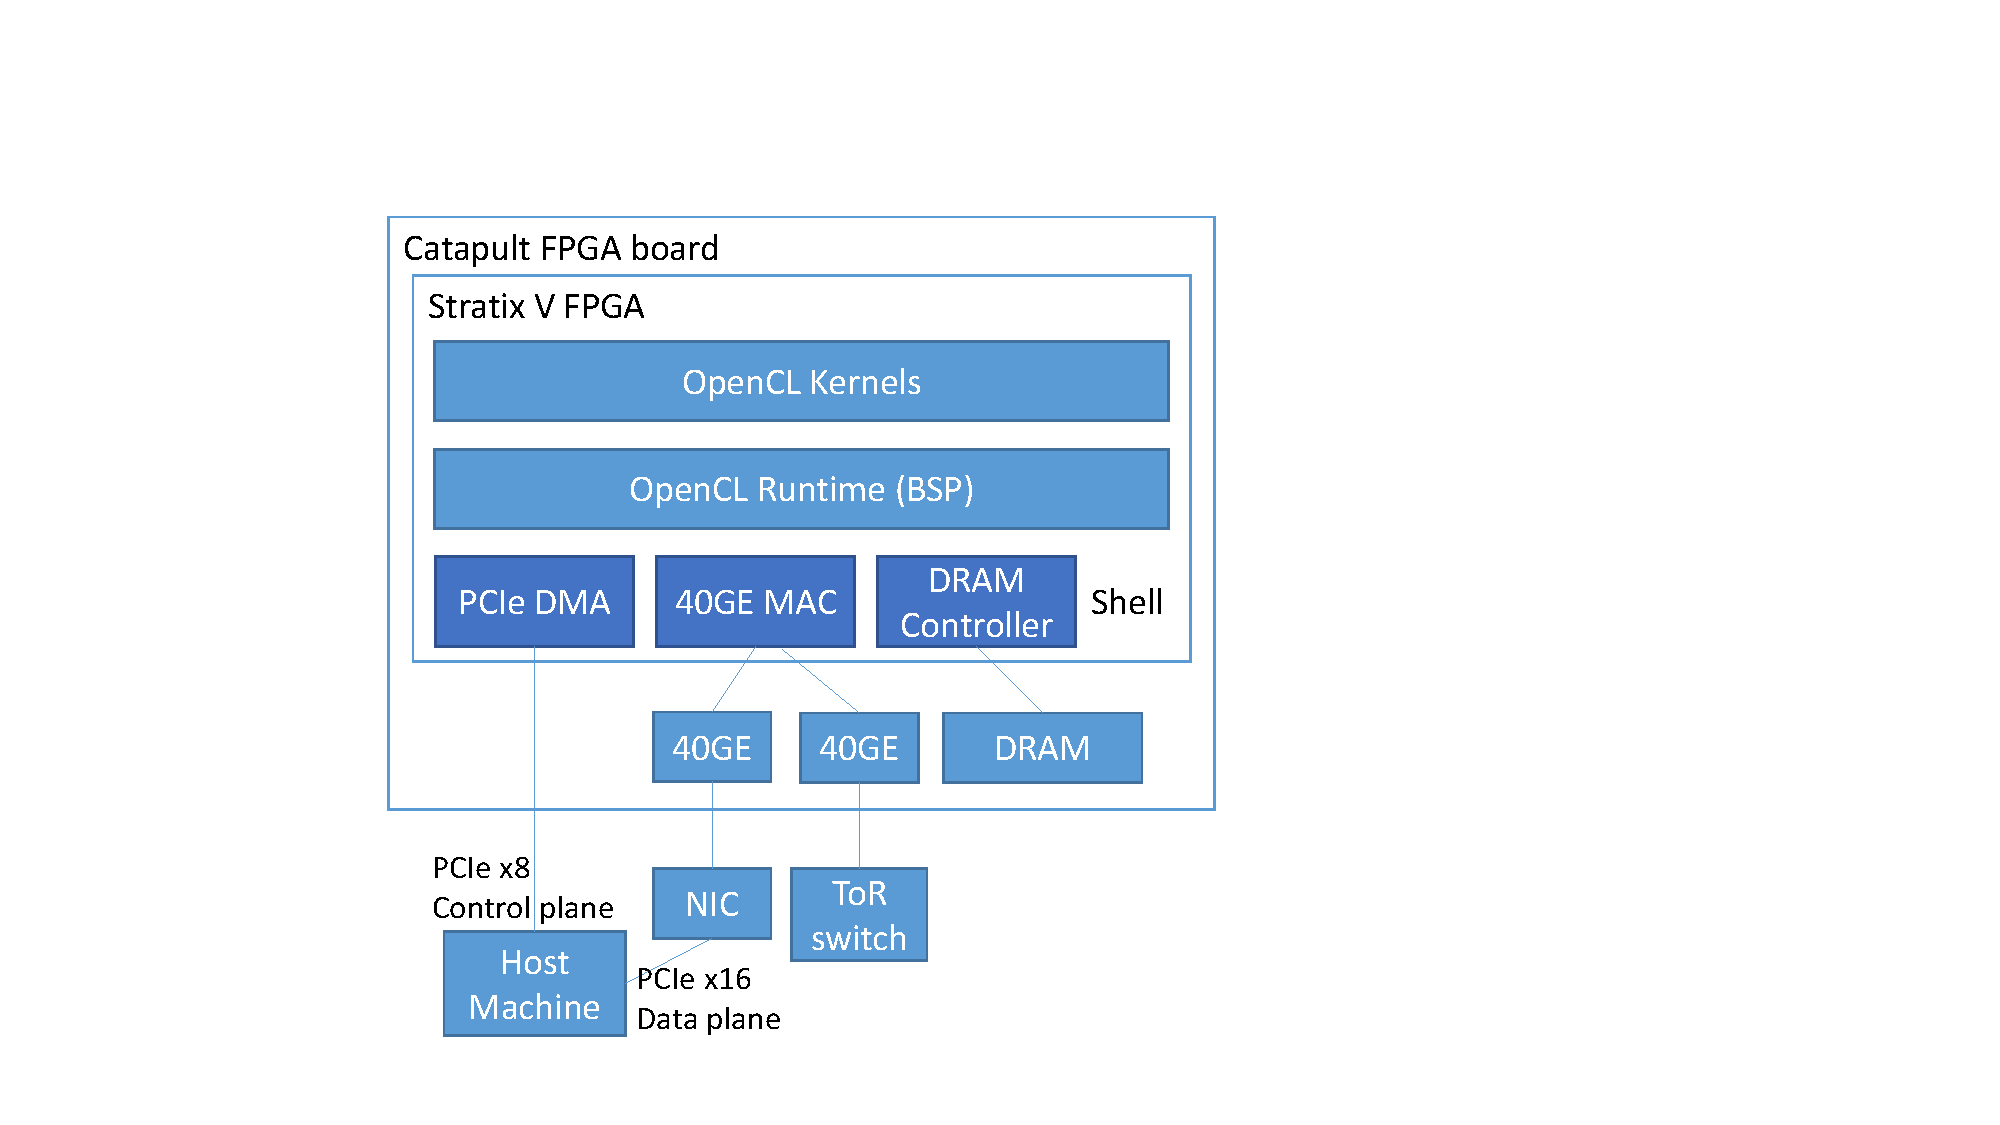
\includegraphics[width=1.0\columnwidth]{image/CatapultFPGAArch}
	\vspace{-0.25in}
	\caption{Catapult FPGA Architecture}
	\vspace{-0.15in}
	\label{fig:CatapultFPGAArch}
	%    \vspace{-2mm}
\end{figure}

In network virtualization scenario, we install one FPGA in each server and connect two 40 GE ports to NIC and Top-of-Rack (ToR) switch respectively. The traffic between NIC and ToR flow through the FPGA to perform comprehensive network functions \textit{bump-in-the-wire}, including tunnel encapsulation and decapsulation, firewall, metering and traffic scheduling. Virtual machines expose to the NIC and FPGA via Single-Root I/O Virtualization (SR-IOV), and data-plane functions of the virtual switch are offloaded to the FPGA.

Current generation of Catapult FPGA has 172,600 ALMs (Adaptive Logic Modules) each containing several 8-input configurable lookup table, two full adders and four one-bit registers \cite{alterafpgaarch}, 2,014 blocks of 20 Kbit SRAM and a 4 GB DRAM. Each register can be read and written every cycle without latency. Each SRAM block can perform one read or write operation with exactly one cycle latency. The performance of DRAM depends on access pattern. When accessed randomly, each operation takes 170 ns (about 34 cycles); when accessed sequentially, the throughput can reach 4 Gbps. Registers, SRAMs and DRAM form a memory hierarchy where faster memory spaces have lower capacity.

\subsection{OpenCL Compiler}

The Altera SDK for OpenCL \cite{singh2011implementing} is a programming framework that abstract away the traditional hardware FPGA development flow. In the OpenCL \cite{khronos2008opencl} model, data-plane functions are wrapped in \textit{kernels} and compiled into hardware accelerators, and control plane on the host machine communicates with kernels via a standard set of APIs. Altera OpenCL introduces \textit{channels} to allow communication among kernels without host intervention.

Central to Altera OpenCL is a compiler \cite{czajkowski2012opencl} that extracts parallelism in OpenCL kernels and generates Verilog code. A parser based on LLVM first parses OpenCL kernel and produces intermediate representation (IR) consisting of instructions and dependencies between them. Then the IR is optimized via live-variable analysis and generate CDFG (Control Data Flow Graph). Based on CDFG, scheduler determines the required clock cycles of each operation, then sequence the operations into a pipeline, where independent operations are parallelized and dependent operations are pipelined. Finally the compiler links to IP library and generates Verilog HDL, as well as a profiling report containing estimated resource utilization and an optimization report containing data dependencies that lead to pipeline stall.

OpenCL is designed primarily for batch processing instead of stream processing, which is a gap that ClickNP needs to bridge. In network stream processing, kernels run in an infinite loop, so the kernels will never finish.

First, when a kernel is running, global memory assigned to it cannot be accessed by the host machine. So commands can not be passed to kernels via global memory on-the-fly. One straightforward approach could be launching another ``proxy'' kernel to pass in commands via channel each time the host sends a command. However, this approach has about 5 millisecond latency due to complicated internals in launching and finishing a kernel. Fortunately, OpenCL only occupies PCIe slots 0--31, so we designed a raw I/O channel via PCIe slots 32--39 to allow on-the-fly interaction of kernels and the host. Figure \ref{fig:PCIeChannelPerf} shows that PCIe I/O channels reach near-theoretical throughput with 5 slots and 16K batch size, and the latency for small batch size is microsecond-scale.

\begin{figure}[h!]
	\centering
	\subfigure[Latency (x: batch size, y: microsec; lines: polling, interrupt, opencl)]{
		
\includegraphics[width=0.45\columnwidth]{image/logo}
		\label{fig:PCIeChannelLatency}
	}
	\subfigure[Throughput (x : number of slots; y: Gbps; lines: batch size, theory)]{
		
\includegraphics[width=0.45\columnwidth]{image/logo}
		\label{fig:PCIeChannelThroughput}
	}
	\vspace{-0.15in}
	\caption{PCIe Channel Performance}
	\vspace{-0.15in}
	\label{fig:PCIeChannelPerf}
	%    \vspace{-2mm}
\end{figure}

Second, since the kernels never finish, when the host program crashes or need to be updated, although the data plane is still running, we might lose the control plane because the kernels may have problem launching again. We added a PCIe-controlled register to trigger reset signal of OpenCL kernel programs and OpenCL runtime on FPGA. When the host program restarts, it toggles the reset register to force stop all kernels and then re-launch them via OpenCL API.

\subsection{ClickNP Toolchain}

The building blocks of ClickNP are \textit{elements}. Each element is compiled to an OpenCL single-work-item \textit{kernel}.

A ClickNP \textit{project} consists of 3 parts: a library of elements, a \textit{Click script} to specify what and how elements are connected, and a \textit{host program} to interact with the user and issue commands to elements.

ClickNP provides 4 build targets for a project:

\begin{enumerate}
	\item Native x86 emulation (in seconds) with ClickNP compiler and standard C++ compiler to test functionality and debug with \textit{printf}.
	\item Generate optimization report (in 1 minute) to understand resource utilization and memory dependencies with ClickNP compiler and OpenCL compiler. If an element is not fully pipelined, or the overall resource utilization is too high, developer should optimize the element code (if a new element is written) or change element parameters (e.g. lookup table size).
	\item Build full FPGA image (in 1--2 hours) with ClickNP compiler, OpenCL compiler and Quartus synthesizer, fitter, assembler and timing analyzer.
	\item Build host program (in seconds) with ClickNP compiler and standard C++ compiler.
\end{enumerate}

%Multiple emulation-mode ClickNP projects can be connected via named pipes, e.g. connect the traffic generator, your bump-in-the-wire ClickNP project and the traffic monitor with pipes to test functionality with various traffic patterns without code modifications.

\begin{figure}[!t]
	\centering
	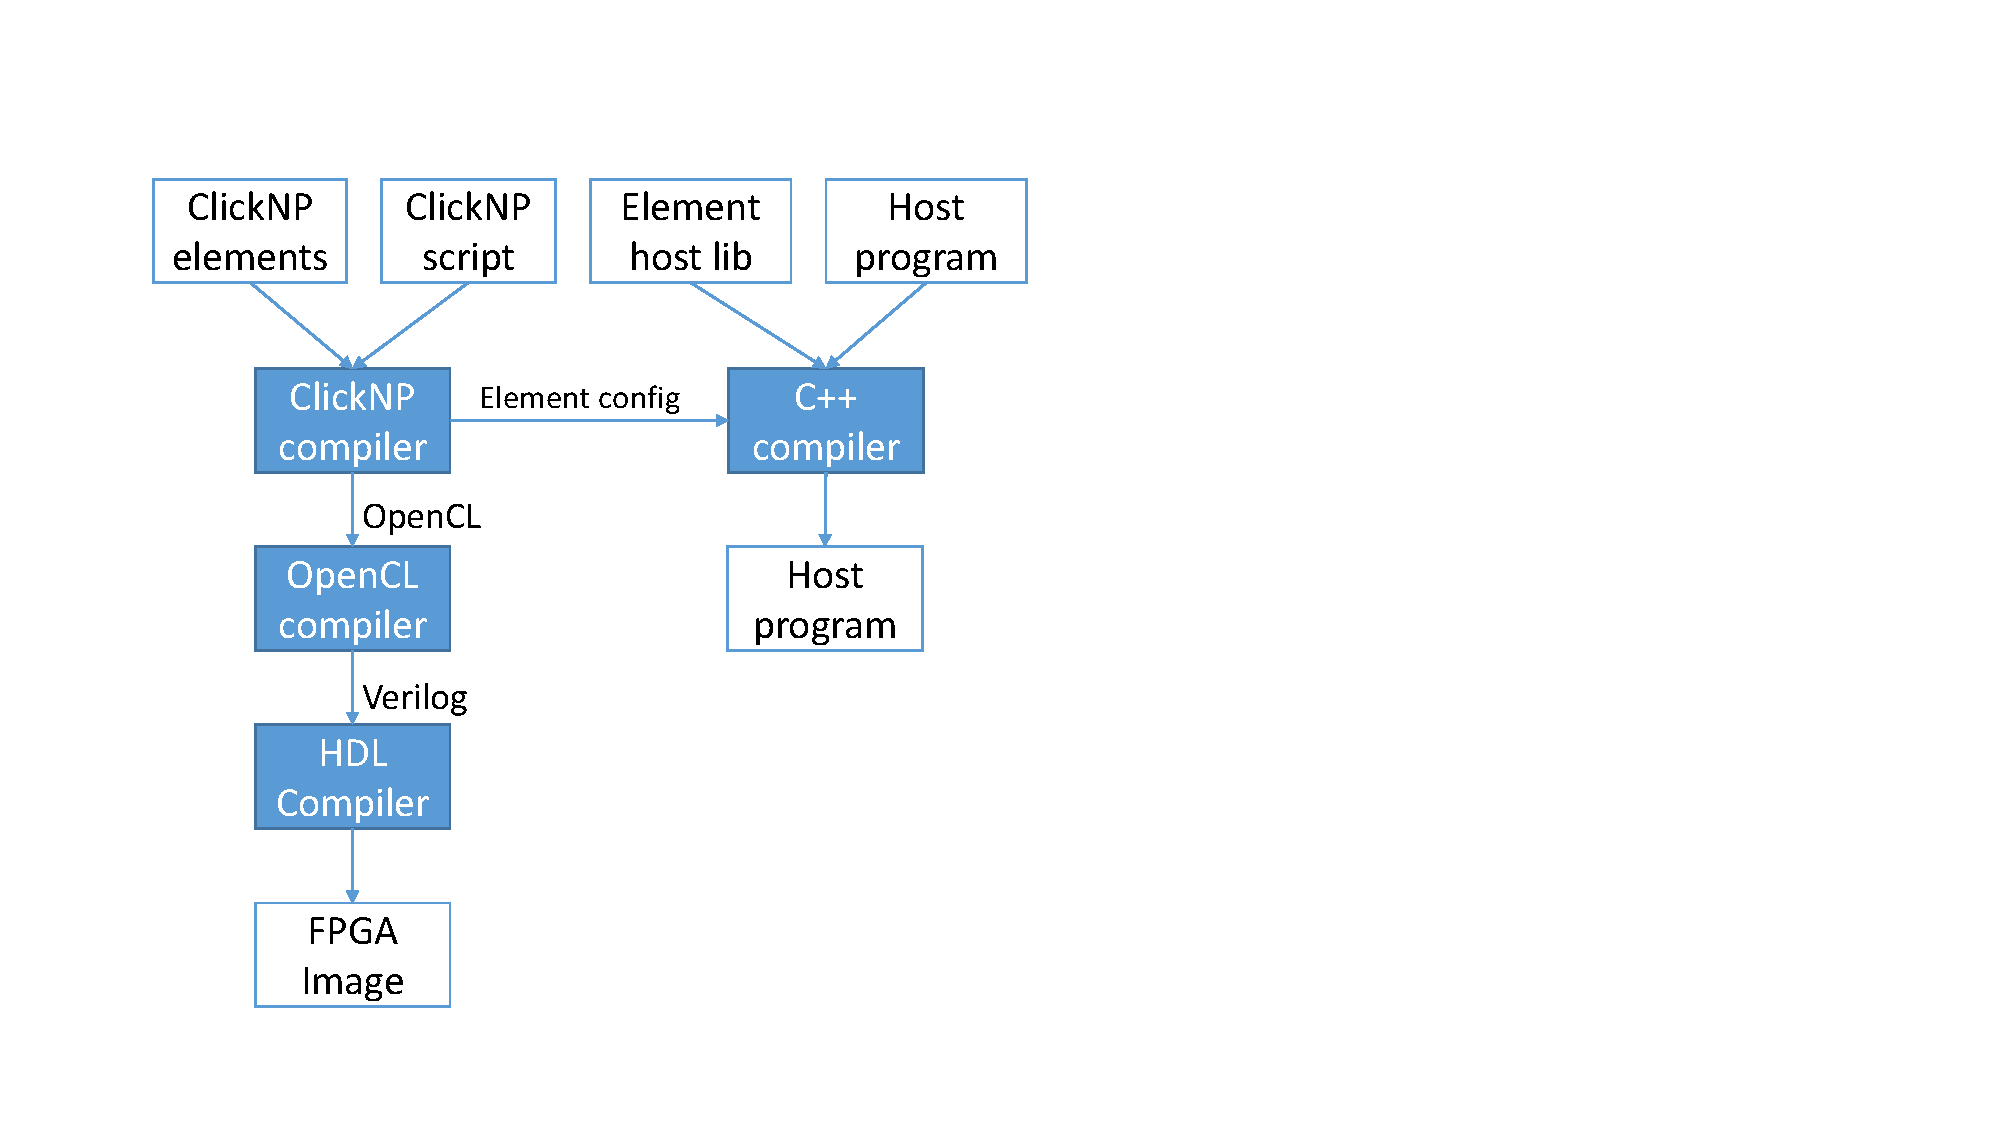
\includegraphics[width=0.8\columnwidth]{image/ClickNPSoftware}
	\vspace{-0.15in}
	\caption{ClickNP Compilation Flow}
	\vspace{-0.15in}
	\label{fig:ClickNPSoftware}
	%    \vspace{-2mm}
\end{figure}

Full compilation of a project generates an FPGA image, a x86 host program and an OpenCL kernel binary. First, the FPGA image is reprogrammed into FPGA via Flash Util in Figure \ref{fig:CatapultFPGAArch} (30 seconds). Second, the host program starts, resets the FPGA board, loads OpenCL kernel binary and launches all kernels. Then the host program keeps running, accepts control plane commands via terminal or RPC, issues signals to elements and listen to events from elements.

When the host program needs to be updated, simply kill the host program and the data plane will keep running. The new host program can choose to either re-initialize all element states, or keep the states and clear in-flight signals and events in case the host program was killed halfway in host-kernel communication.

\begin{figure}[!t]
	\centering
	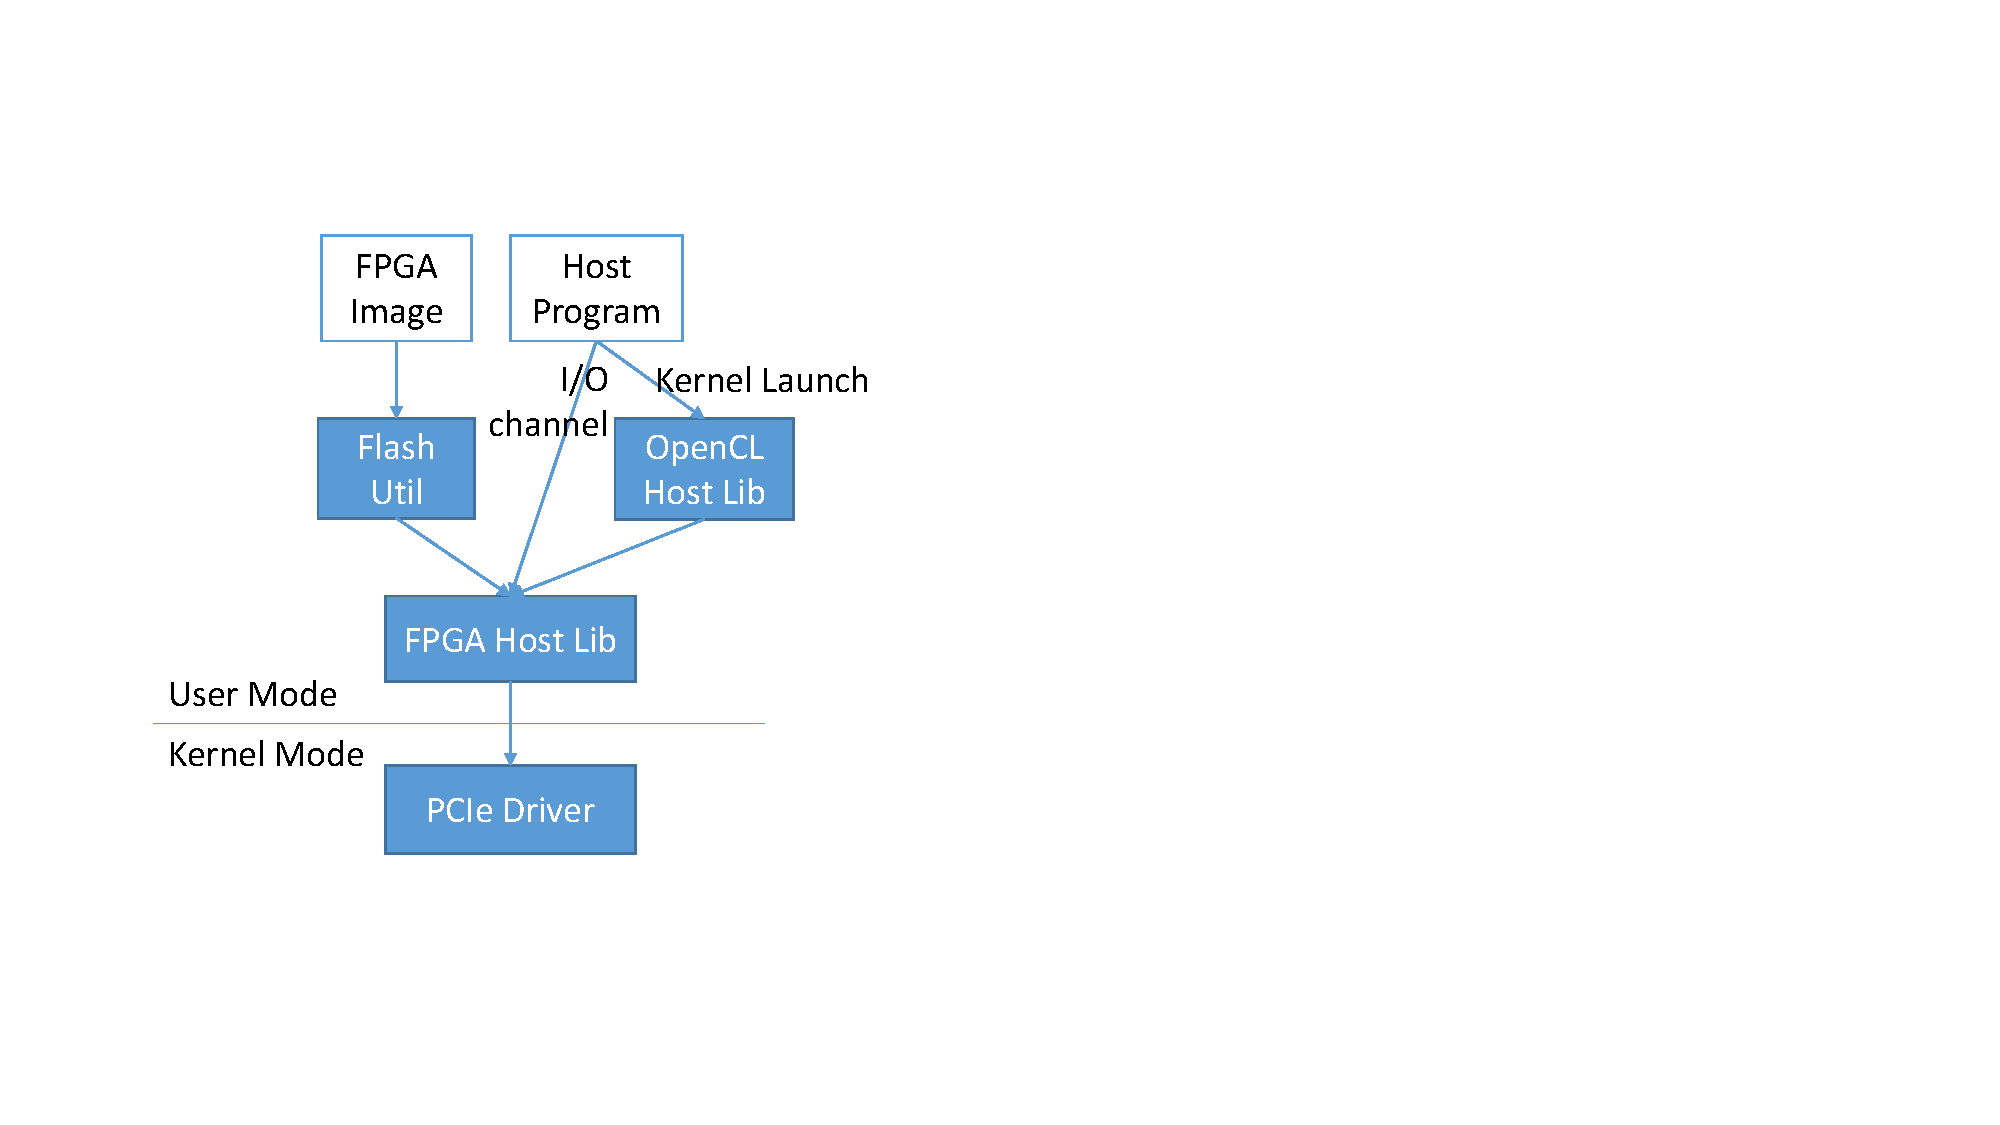
\includegraphics[width=0.8\columnwidth]{image/CatapultRuntime}
	\vspace{-0.15in}
	\caption{ClickNP Runtime Architecture}
	\vspace{-0.15in}
	\label{fig:CatapultFPGAArch}
	%    \vspace{-2mm}
\end{figure}
}

%!TEX root=main.tex
\section{Parallelizing in FPGA}
\label{sec:optimization}

As discussed in \S\ref{subsec:fpga}, it is critical to fully utilize the parallelism inside FPGA in order to speed up processing.
\name\ exploits FPGA parallelism both at element-level and inside an element.

\subsection{Parallelism across elements}

The modular architecture of \name\ makes it natural to exploit parallelisms across different elements.
The \name\ tool-chain maps each element into a hardware block in FPGA. 
These logic blocks are interconnected with FIFO buffers, and can work completely in parallel.
%
To this end, one can think of each element in a \name\ configuration as a tiny, independent core with customized logic.
Packets flow from one element to another along a \textit{processing pipeline}.
This type of parallelism is called \textit{pipeline parallelism} or \textit{task parallelism}. % (Figure~\ref{fig:element-para}(a)).
%
Furthermore, if a single processing pipeline does not have enough processing power, we can duplicate multiple such pipelines 
in FPGA and divide data into these pipelines using a load-balancing element, \ie, exploiting \textit{data parallelism}. %(Figure~\ref{fig:element-para}(b)).
For network traffic, there are both data parallelism (at packet-level or flow-level)
and pipeline parallelism that can be utilized  to speed up processing.
\name\ is very flexible and can be configured to capture both types of parallelism with little efforts.

\egg{
\begin{figure}
\centering
\begin{tabular}{c}
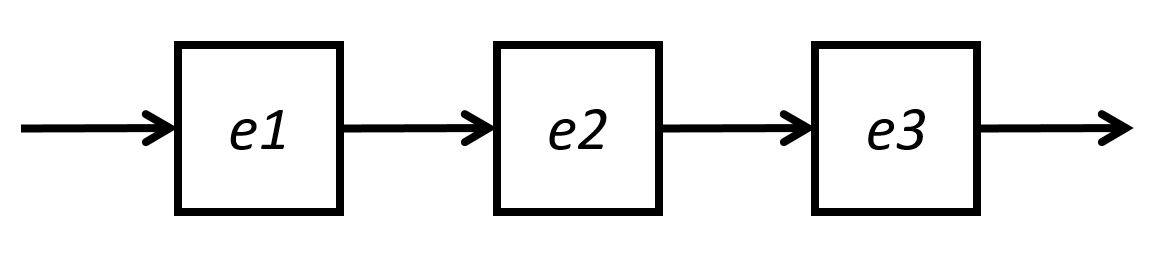
\includegraphics[width=0.28\textwidth]{pipeline.jpg}\\
(a)\\
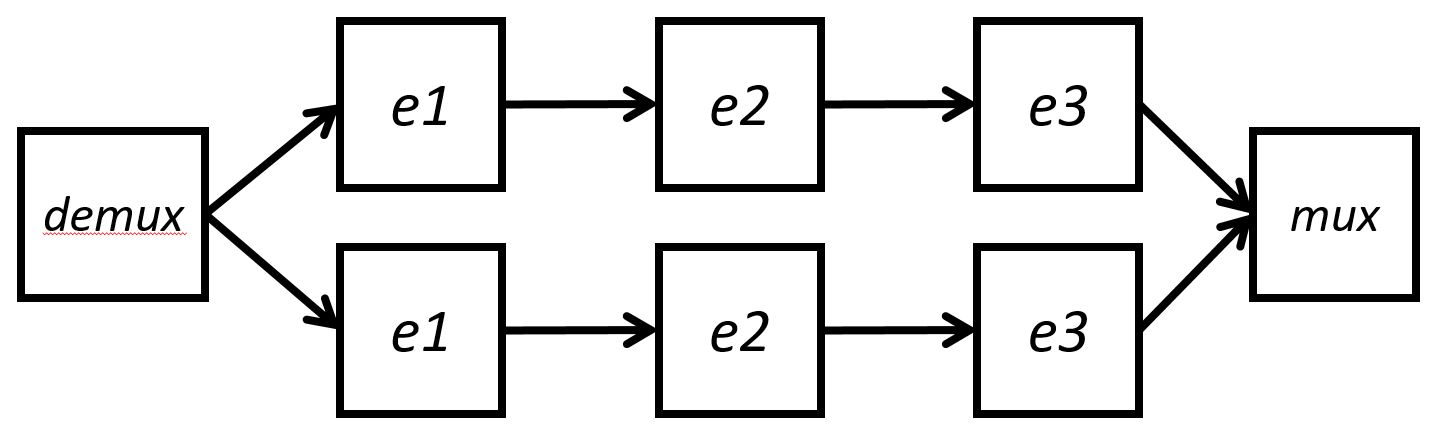
\includegraphics[width=0.35\textwidth]{data.jpg}\\
(b)\\
\end{tabular}
\caption{(a) Pipeline parallelism among elements. (c) Data parallelism among elements.}
\label{fig:element-para}
\end{figure}
}

\subsection{Parallelism inside element}
\label{subsec:paral_in_elem}

%
% We need to get the processing pipeline concept clear here.
%
Unlike CPU, which executes instructions in memory with limited parallelism, 
FPGA synthesizes operations into hardware logic, and therefore
can be evaluated in parallel without instruction load overhead.
If a datum requires multiple dependent
operations in one handler function, HLS tools will 
schedule these operations into pipeline stages in a synchronized manner. 
At every clock, the result of one stage moves to the next stage, and 
at the same time, a new datum is inputed into this stage, as shown in
Figure~\ref{fig:dependency}(a).
This way, the handler function can process a datum at every clock cycle
and achieve maximum throughput.
%
However, in practice, this efficient pipeline processing 
could break under two situations: (1) there is \textit{memory dependency} among operations; 
and (2) there are \textit{unbalanced} stages.
%
In the following two subsections, we will discuss these two issues in 
details and present our solutions.
%Finally, in \S~\ref{subsubsec:pipeline-control}, we discuss how to explicitly
%control the pipelining to get better clock frequency in \name.



\subsubsection{Minimize memory dependency}

\begin{figure}
\lstset{style=numbers}

\lstset{ emph={%
 element, init, state, handler, signal,include
}, emphstyle={\bfseries .},
morekeywords={get_input_port,read_input_port,from_tor, to_tor, set_output_port, host} 
}

\centering
\begin{tabular}{c}

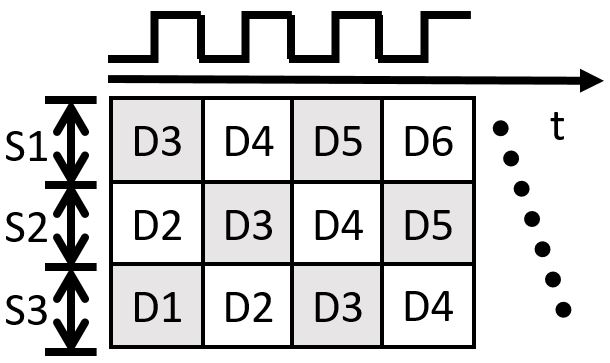
\includegraphics[width=.25\textwidth]{pipeline-w-data.jpg} \\
(a) \vspace{3pt} \\
{
\scriptsize 
\begin{lstlisting}[escapechar=@]
    r = read_input_port (PORT_1);
S1: y = mem[r.x]+1;
S2: mem[r.x] = y;
    set_output_port (PORT_1, y);
\end{lstlisting} 
}\\
(b) \vspace{3pt}\\
{
\scriptsize 
\begin{lstlisting}[escapechar=@]
    r = read_input_port (PORT_1);
P1: if ( r.x == buf_addr ) {
       y_temp = buf_val;
    } else {
       y_temp = mem[r.x];
    }
    mem[buf_addr] = buf_val;   
S1: y = y_temp + 1;
S2: buf_addr = r.x;
    buf_val  = y;
    set_output_port (PORT_1, y);
\end{lstlisting} 
}\\
(c)
\end{tabular}
\caption{Illustration of dependency. (a) No dependency. S$n$ means a pipeline stage, D$n$ is a datum. (b) Memory dependency occurs when states are stored in memory and need to be updated. (c) Resolve memory dependency using delayed write.}
\vspace{-10pt}
\label{fig:dependency}
\end{figure}

% registers
\egg{
\smalltitle{Use registers.}
Unlike CPU, which executes instructions in memory one by one, FPGA synthesizes 
operations into hardware logic and stores data in registers, and therefore 
can be evaluated in parallel.
For example, Figure~\ref{fig:dependency}(a), it may take a CPU two cycles 
to execute \textbf{S1} and \textbf{S2}, while in FPGA, the value of variable 
\textit{y} and \textit{z} can be evaluated in one cycle using 
combinational logic, if we store all variables in registers.
FPGA usually has a large number of registers, \ie, 697Kbit for Altera 
Stratix V, and therefore \name\ aggressively assigns scalar variables 
using registers to increase the parallelism.
}

%\smalltitle{Minimize memory dependency.}
If two operations access the same memory location, and at least one of them
is \textit{write}, we call these two operations depend on each other~\cite{dependence}. 
Operations with \textit{memory dependency} cannot be evaluated at the same time,
as each memory access has one cycle latency and the semantic correctness of the program strongly depends on the order
of operations.
%
As shown in Figure~\ref{fig:dependency}(b), \textbf{S1} and \textbf{S2}
depend on each other: \textbf{S2} has to be delayed until \textbf{S1} finishes, 
and only after \textbf{S2} finishes can \textbf{S1} operate on new input data.
Therefore, the function will take two cycles to process one datum.
%
Memory dependency can be rather complicated for some processing algorithms,
but thanks to the modular architecture of \name, most elements perform 
only simple tasks and the \textit{read-write} memory dependency shown in 
Figure~\ref{fig:dependency}(b) is the most common case we have encountered.

One way to remove this memory dependency is to store data in registers only. 
%
Since registers are fast enough to perform read, computation and write back within one cycle,
there would be no \textit{read-write} dependency at all. 
Indeed, compared to CPU, FPGA has a much larger number of 
registers, \ie, 697Kbit for Altera Stratix V, which can be used
whenever possible to reduce memory dependency.
The \name\ compiler aggressively assigns registers to variables as long as
all accesses to the variable refer to a constant address -- either the variable is a scalar or an array entry with constant offset.
%
Certainly, the programmer can use ``register'' or ``local/global'' keywords to explictly instruct the compiler to place a variable (can also be an array)
in register, BRAM or onboard DDR memory.
%declare the  in array declaration to force the compiler to use registers and generate multiplexers for memory access.}

For large data, they have to be stored in memory. 
%
Fortunately, we can still use a technique called \textit{delayed write} to
resolve the \textit{read-write} memory dependency in Figure~\ref{fig:dependency}(b).
The core idea is to buffer the new data in a register and delay the write
operation until the next read operation. 
If the next read accesses the same location, it will read the value from
the buffer register directly. Otherwise, the read can operate in parallel 
with the delayed write operation as they are going to access different
memory locations\footnote{Most BRAM in FPGA has two ports.}.
Figure~\ref{fig:dependency}(c) shows the code snippet with delayed write.
Since there is no longer memory dependency in the code, the element can 
process a datum in one cycle.
%
By default, \name\ compiler automatically applies \textit{delayed write} 
for an array (generating similar code as shown in Figure~\ref{fig:dependency}(b)).
%
\egg{But Currently the compiler can generate only one delayed write per array.
For complex memory dependencies, the programmer should rewrite the code into multiple elements accessing disjoint memory regions, and use message-based coordination if necessary.}


\begin{figure}
\lstset{style=numbers}

\lstset{ emph={%
 element, init, state, handler, signal,include,state\_machine, goto_state
}, emphstyle={\bfseries},
morekeywords={get_input_port,read_input_port,from_tor, to_tor, set_output_port, host, begin, VLAN, IPv4, GRE} 
}
\centering


\begin{tabular}{cc}
\scriptsize 
\begin{lstlisting}[escapechar=@]
struct hash_entry
{
  ulong key;
  ulong cnt;
} A[100];

.handler {
  ...
  idx = hash (h);
S1: if (A[idx].key==k)
  {
S2: A[idx].cnt ++;
  }
  ...
}
\end{lstlisting} &
\raisebox{-60pt}{
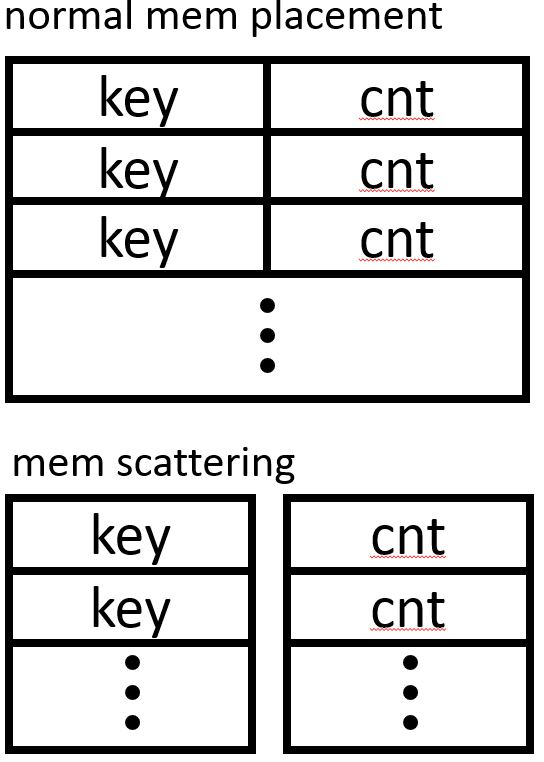
\includegraphics[width=.17\textwidth]{mix.jpg} }\\
(a) & (b)
\end{tabular}
\vspace{-10pt}
\caption{Memory scattering. }
\vspace{-15pt}
\label{fig:memscattering}
\end{figure}


%\smalltitle{Remove pseudo-dependency.}
One subtle issue will occur when using an array of \textit{struct} variables. 
Figure~\ref{fig:memscattering}(a) shows such an example, where
a hash table is used to maintain a count for every flow.
We find \textbf{S2} will have a memory dependency to \textbf{S1}, although
they are accessing different fields of a \textbf{struct}.
The reason is that almost all current HLS tools will treat a \textbf{struct}
array as a single-dimension array with a large bit-width -- equal to
the size of the \textbf{struct}, and use only one arbitrator to control 
 access.
We call this type of memory dependency \textit{pseudo dependency}, 
as physically, the two fields, \textit{key} and \textit{cnt}, can be on different 
memory locations.
%
To resolve this issue, \name\ employs a simple technique called \textit{memory scattering}, which automatically 
translates a \textbf{struct} array into several 
independent arrays, each for a field in the \textbf{struct}, and assigns them into different BRAMs (Figure~\ref{fig:memscattering}(b)).
With \textit{memory scattering}, \textbf{S1} no longer depends on \textbf{S2}.
So the pipeline can be inferred by HLS tools, and when \textbf{S2} is 
still operating, a new datum can be clocked in and processed 
by \textbf{S1}.
It is worth noting that memory scattering is only applied for elements 
in FPGA and disabled if elements are assigned to run on the host CPU.

We note that the above techniques may not resolve all memory dependencies. 
In many cases, it requires programmers to re-factor their code or even change
the algorithms to ensure their implementation can be fully pipelined in FPGA. 

\egg{
\begin{figure}
\lstset{style=numbers}

\lstset{ emph={%
 element, init, state, handler, signal,include,state\_machine, goto_state
}, emphstyle={\bfseries},
morekeywords={get_input_port,read_input_port,from_tor, to_tor, set_port_output, host, begin, VLAN, IPv4, GRE} 
}
\centering

\begin{tabular}{c|c}
% left
\begin{tabular}[t]{c}
\scriptsize 
\begin{lstlisting}[escapechar=@]
struct hash_entry
{
    ulong key;
    ulong val;
} A[100];

.handler {
   ...
   idx = hash (h);
   @\textbf{k = A[idx].key;}@
   @\textbf{v = A[idx].val;}@
   if (h == k) 
      ret = v;
   ...
}
\end{lstlisting} \\
\normalsize (a) \vspace{10pt} \\
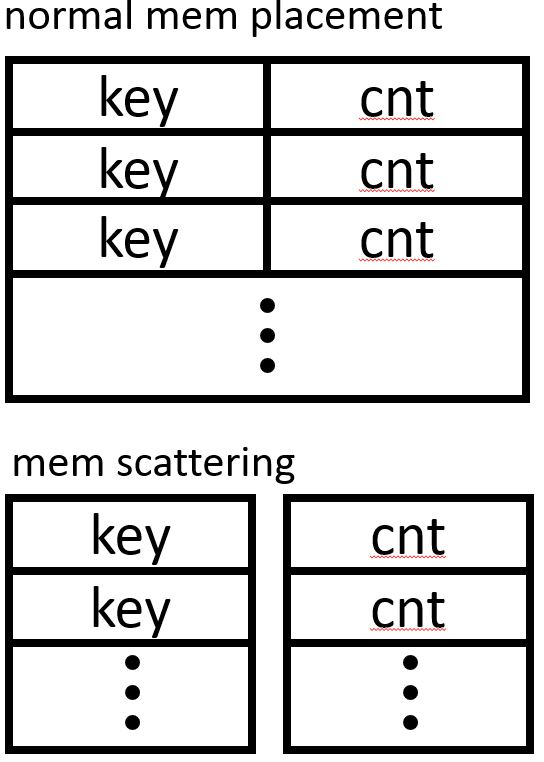
\includegraphics[width=.2\textwidth]{mix.jpg} \\
\normalsize (b) \vspace{10pt} \\
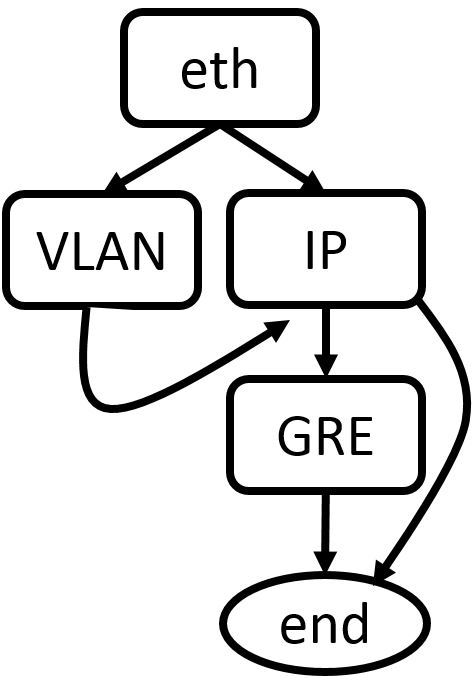
\includegraphics[width=.15\textwidth]{fsm1.jpg} \\
\normalsize (d) \\
\end{tabular}
&
\raisebox{-150pt}{
\begin{tabular}{c}
\begin{lstlisting}[escapechar=@]
.handler {
 ...
 .state_machine
 {
  begin { // ethernet
   ...
   if(etype==0x8100)
    .goto_state VLAN;
   else 
   if(etype==0x0800)
    .goto_state IPv4;
   else
    .goto_state end;
  }
  VLAN {
    ...
    if(etype==0x0800)
     .goto_state IPv4;
    else
     .goto_state end;
  }
  IPv4 {
    ...
    if(proto==0x2F)
     .goto_state GRE;
    else
     .goto_state end;
  }
  GRE {
   .goto_state end;
  }
 }  
...
}

\end{lstlisting}  \\
\normalsize (c) \vspace{10pt} \\
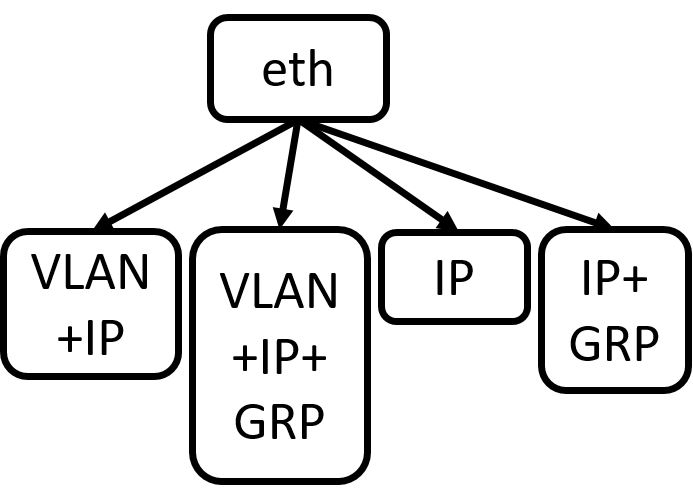
\includegraphics[width=.2\textwidth]{fsm2.jpg} \\
\normalsize (e) \\
\end{tabular}
}

\end{tabular}

\caption{Memory scattering (a, b) and FSM expansion (c-e). }
\label{fig:memscattering}
\end{figure}
}

\subsubsection{Balance pipeline stages}
Ideally, we require every stage in one processing pipeline to have the same speed. \ie, processing a datum at one clock cycle.
However, if the process at each stage is unbalanced and some stages need more cycles than others, these fat stages will
limit the whole throughput of the pipeline.  
For example, in Figure~\ref{fig:unbalance}(a), \textbf{S1} is a loop operation. 
Since each iteration takes one cycle (\textbf{S2}), the whole loop will need $N$ cycles to finish, significantly reducing the pipeline
throughput.
Figure~\ref{fig:unbalance}(b) shows another example, which implements a cache in BRAM for a global table (\textit{gmem}) in DDR.
Although the ``else'' branch is seldom hit, it generates a fat stage in the 
pipeline (taking hundreds of cycles!), and slows down
the processing greatly.

\name\ uses two techniques to balance the stages inside a pipeline. First, we \textit{unroll} the loop whenever possible. 
When unrolled, the loop operation effectively breaks into a sequence of small operations, each of which can be finished in one cycle.
It is worth noting that unrolling a loop will duplicate the operations in the loop body and thus increase area cost. 
Therefore, it may be only applicable to loops with simple bodies and 
small number of iterations. 
In NFs, we find such small loops are rather common, \eg calculating checksums, shifting packet payload and iterating through possible configurations.
ClickNP compiler provides the \textbf{.unroll} directive to unroll a loop. 
%
While many HLS tools support loop unroll for a known number of iterations, 
ClickNP extends this capability to unroll a loop whose  
number of iterations is unknown but under an upper bound 
that is specified by programmers.

Second, if we identify that an element has both heavy and light-weight operations, we try to separate each type of operations in an individual element.
For example, to implement a cache as shown in Figure~\ref{fig:unbalance}(b), we move the slow ``else'' branch into another element.
This way, the fast path and the slow path would be running asynchronously.
If cache miss is rare, the overall processing speed is dominated by the fast path.
We will return to this point later in \S\ref{sec:application}.
Currently, \name\ compiler cannot automatically perform such separation for 
programmers.

\begin{figure}
\lstset{style=numbers}

\lstset{ emph={%
 element, init, state, handler, signal,include,state\_machine, goto_state
}, emphstyle={\bfseries},
morekeywords={get_input_port,read_input_port,from_tor, to_tor, set_output_port, host, begin, VLAN, IPv4, GRE} 
}
\centering

\begin{tabular}{c}
{
\scriptsize 
\begin{lstlisting}[escapechar=@]
.handler {
   r = read_input_port (PORT_1);
   ushort *p = (ushort*) &r.fd.data;
S1:for (i = 0; i<N; i++) {
S2:  sum += p[i];
   }
}
\end{lstlisting} 
} \\
(a) \vspace{3pt} \\
{
\scriptsize 
\begin{lstlisting}[escapechar=@]
.handler {
   r = read_input_port (PORT_1);
   idx = hash (r.x);
S1:if ( cache[idx].key == r.x ) {
     o = cache[idx].val;
S2:} else {
     o = gmem[r.x];
     k = cache[idx].key;
     gmem[k] = cache[idx].val;
     cache[idx].key = r.x;
     cache[idx].val = o;
   }
   set_output_port (PORT_1, o);
}
\end{lstlisting} 
} \\
(b) \vspace{3pt} 
\end{tabular}

\caption{Unbalanced pipeline stages. }
\label{fig:unbalance}
\vspace{-10pt}
\end{figure}


\egg{
\smalltitle{Expand code.} \name\ provides several tools to help programmers to expand code, trading off FPGA area for speed.
One common code expansion is to unroll loops. Additionally, \name\ provides \textit{.repeat} directive to expand code according to
a template.
Finally, \name\ can also help to expand a \textit{finite state machine} (FSM).
Figure~\ref{fig:memscattering}(c) shows such an example in packet header parser.
The \textbf{.state\_machine} directive has two functions. First, it provides programmers a declarative way to write a FSM by defining
states and their transitions (using \textbf{.goto\_state}).
Second, it also expends the FSM to get more parallelism. 
For example, Figure~\ref{fig:memscattering}(d) shows the parsing tree that is described according to the code piece in Figure~\ref{fig:memscattering}(c).
But \name\ compiler can automatically expends the FSM to an equivalent, but much flattened FSM, as shown in Figure~\ref{fig:memscattering}(e). Now every header can be parsed in one cycle -- all parsing paths can be evaluated in parallel, 
instead of up to 4 cycles (Figure~\ref{fig:memscattering}(d)).
}

\egg{
\subsubsection{Explict pipeline control}
\label{subsubsec:pipeline-control}

While commercial HLS tools can automatically generate pipeline structure, it is not always perfect. 
One issue that we are facing occasionally is that HLS tools may too aggressively use large block of combinational logic 
to implement operations in a handler function.
Although packing more operations in a combinational logic makes all these operations be evaluated in parallel in one clock,
it may also reduce the clock frequency of the FPGA as the frequency is restricted by the delay of the logic block, and larger
the block, longer the delay.
%
For example, Figure~\ref{fig:pipeline-control}(a) shows such an example. The code snippet selects the maximal value from
a set of registers (as we will show later, this is a foundation for priority scheduling).
Since all data are in registers, most HLS tools will aggressively use a large block of combinational logic to implement, so that
all \textbf{if} operations are evaluated in one clock cycle. However, this will cause a low frequency of xxx MHz. 
As shown in Figure~

}
%!TEX root=main.tex
\section{Implementation}
\label{sec:impl}

\subsection{\name\ tool-chain and hardware setup}
We have built a \name\ compiler which serves as the front-end of the \name\ tool-chain (\S\ref{subsec:toolchain}).  
%
For the host program, we use Visual C++ as the backend. We further integrate Altera OpenCL SDK (v15.1)~\cite{aoc} and 
Xilinx Vivado HLS (v2015.4)~\cite{vivado} as the backend for the FPGA program.
%
The \name\ compiler contains 4,925 lines of C++ code, which parses configuration file and element declarations, 
performs optimizations in \S\ref{sec:optimization}, and generates code specific for each commercial HLS tool.
% Cross platform.
When working with Altera OpenCL, each \name\ element is compiled into a \textit{kernel} and 
the connections between elements are translated into Altera extended channels.
When using Xilinx Vivado HLS, we compile each element into an IP core and 
use AXI streams to implement connections between elements.
%
An element can also be compiled to CPU binary and the manager thread will create one worker thread for each host element.
%
Each connection between a host and a FPGA element is mapped to a \textit{slot} of the PCIe I/O 
channel (\S\ref{subsec:pcie}).

Our hardware platform is based on Altera Stratix V FPGA with the Catapult shell~\cite{putnam2014reconfigurable}.
The Catapult shell also contains an OpenCL specific runtime, so that the \name\ role can communicate with the shell 
through this runtime layer.
The FPGA board has a PCIe Gen2 x8 interface, 4GB onboard DDR memory and two 40G Ethernet ports. 
%
By the time of writing this paper, we do not get a Xilinx hardware platform. 
Therefore, the primary system evaluations are based on the Altera platform using \name+OpenCL, 
and we use the reports generated by Vivado HLS, \eg, frequency and area cost, to understand 
the performance of \name+Vivado.

\subsection{\name\ element library}
\label{subsec:lib}

\begin{table*}[t!]
	\centering
	\caption{A selected set of key elements in \name. }
	\label{tab:elements}
	\scalebox{0.9}{
		\begin{tabular}{l|l|l|p{1cm}|p{2.2cm}|p{2cm}|p{1.3cm}|r|r}
			\toprule
			&	&	& \multicolumn{4}{c|}{Performance} & \multicolumn{2}{c}{Resource (\%)} 			\\
			\cline{4-7} \cline{8-9}  

 Element 	& Configuration & Optimizations & Fmax (MHz) & Peak \quad \quad Throughput & Speedup\quad (FPGA/CPU) & Delay (cycles) & LE & BRAM \\
			\midrule
			L4\_Parser (A1-5)  & N/A & REG & 221.93 & 113.6 Gbps & 31.2x / 41.8x & 11 & 0.8\% & 0.2\% \\
			IPChecksum (A1-4) & N/A & UL & 226.8 & 116.1 Gbps & 33.1x / 55.1x & 18 & 2.3\% & 1.3\% \\
			NVGRE\_Encap (A1,4) & N/A & REG, UL & 221.8 & 113.6 Gbps & 35.5x / 42.9x & 9 & 1.5\% & 0.6\% \\
			\midrule
			AES\_CTR (A3) & 16B block & UL & 217.0 & 27.8 Gbps & 79.9x / 255x & 70 & 4.0\% & 23.1\% \\
			SHA1 (A3) & 64B block & MS, UL & 220.8 & 113.0 Gbps & 157.5x / 83.1x & 105 & 7.9\% & 6.6\% \\
			\midrule
			\midrule
			CuckooHash (A2) & 128K entries & MS, UL, DW & 209.7 & 209.7 Mpps & 43.6x / 57.5x & 38 & 2.0\% & 65.5\% \\
			HashTCAM (A2) & 16 x 1K & MS, UL, DW & 207.4 & 207.4 Mpps & 155.9x / 696x & 48 & 18.7\% & 22.0\% \\
			LPM\_Tree (A2) & 16K entries & MS, UL, DW & 221.8 & 221.8 Mpps & 34.5x / 45.2x & 181 & 4.3\% & 13.2\% \\
			FlowCache (A4) & 4-way, 16K & MS, DW & 105.6 & 105.6 Mpps & 55.8x / 21.5x & 27 & 5.6\% & 46.9\% \\
			\midrule

			SRPrioQueue (A5) & 32 Pkts buffer & REG, UL & 214.5 & 214.5 Mpps & 150.3x / 28.6x & 41 & 2.6\% & 0.6\% \\
			RateLimiter (A1,5) & 16K flows & MS, DW & 141.5 & 141.5 Mpps & 7.0x / 65.3x & 14 & 16.9\% & 14.1\% \\
\bottomrule

	\multicolumn{9}{l} {\textbf{Optimization method.} REG=Using Registers; MS=Memory Scattering; UL=Unroll Loop; DW=Delay Write.} \\
	\multicolumn{9}{l} {\parbox{\textwidth}{The \textbf{Speedup} column compares the performance between
	the optimized version and our earlier implementation without applying techniques discussed in \S\ref{sec:optimization} as well as a CPU implementation.}}

\vspace{-15pt}		\end{tabular} 

	}
\end{table*}

We have implemented a \name\ element library that contains nearly 100 elements. 
Part of them (20\%) are derived directly from the Click Modular Router, 
but re-factored using the \name\ framework. 
These elements cover a large range of basic operations of NFs, 
including packet parsing, checksum computing,
encap/decap, hash tables, longest prefix matching (LPM), 
rate limiting, cryptographic, and packet scheduling. 
%
Due to the modular architecture of \name, the code size of each element is modest. 
The mean line-of-code (LoC) of an element is 80 and 
the most complex element, \textit{PacketBuffer}, has 196 lines of C code. 
% 
Table~\ref{tab:elements} presents a selected set of key elements we have implemented in \name. 
Beside element names, we also mark the demonstration NFs (A1\approx A5, discussed in \S\ref{sec:application}) in 
which the element is used.
%
We have heavily applied the optimization techniques discussed earlier in \S\ref{subsec:paral_in_elem} to 
minimize memory dependency and balance pipeline stages.
We summarize the optimization techniques used for each element in the 3rd column.
For the top part of Table~\ref{tab:elements}, the element needs to touch every byte of a packet. We show the throughput in Gbps.
The elements in the bottom part of the table, however, process only the packet header (metadata). Therefore, it makes more
sense to measure the throughput using packet per second.
%
We note that the throughput measured in Table \ref{tab:elements} is the maximal throughput that the corresponding element can achieve.
When they work in a real NF, other components, \eg the Ethernet port, may be the bottleneck.
%
As a reference, we compare the optimized version to our earlier  
implementation on FPGA without applying the techniques discussed in \S\ref{sec:optimization} as well as a CPU implementation.
Clearly, after optimization, all these elements can process packet very efficiently, achieving 7\approx 157x speedup compared to our naive FPGA implementation, and 21\approx 696x speedup over a software implementation on one CPU core.
This performance gain comes from the ability to utilize the vast parallelism in FPGA.
%
Considering the power footprint of FPGA (\approx 30W) and CPU (\approx 5W per core), 
\name\ elements are 4\approx 120x more power efficient than CPU. 

We also show the processing latency of each element in Table~\ref{tab:elements}. 
As we see, this latency is low: The mean is $0.19 \mu s$ and the maximum is merely $0.8 \mu s$ (LPM\_Tree).
% cost
The last two columns summarize the resource utilization of each element. The utilization is normalized to
the capacity of the FPGA chip. 
We can see most elements use only a small number of logic elements.
This is reasonable as most operations on packets are simple. 
HashTCAM and RateLimiter have moderate usage of LEs because these elements have larger arbitration logic. 
%
The BRAM usage, however, heavily relies on configurations of elements. For example, the BRAM usage grows linearly 
with the number of entries supported in a flow table. 
Overall, our FPGA chip has sufficient capacity to support a meaningful 
NF containing a handful elements (\S\ref{sec:application}).



\subsection{PCIE I/O channel}
\label{subsec:pcie}

As aforementioned, one key property of \name\ is to support joint CPU/FPGA processing. 
We enable this by designing a high-throughput, low latency PCIe I/O channel. 
%
We extend the OpenCL runtime and add a new I/O channel, which is connected to 
a PCIe switch in the shell. 
The PCIe switch will arbitrate the access between the newly added I/O channel
and other components in the shell, \eg, DDR memory controller.

We leverage the PCIe slot DMA engine in Catapult shell \cite{putnam2014reconfigurable}, which divides a PCIe Gen2 x8 link into 64 logical sub-channels, \ie, \textit{slots}.
Each slot has a pair of send and receive buffers for DMA operations.
%
Among 64 slots, 33 are reserved by Shell and the runtime library to control kernels and access on-board DDR, one slot is used for passing signals to \name\ elements. 
The remaining 30 slots, however, are used for data communications among FPGA and CPU elements.
%
To amortize DMA overhead, we aggressively use \textit{batching}. The maximum message size 
is limited at 64KB. 
%The PCIe channel can work in both interrupt or polling mode.



% cmdhub
In FPGA, a special element, called \textit{CmdHub}, which is generated automatically by the \name\ compiler, 
redirects the data from different slots to corresponding FPGA elements 
using FIFO buffers.
% signal slot
\textit{CmdHub} is also used to distribute control signals from the manager 
thread to FPGA elements.
To identify the target element, an element ID is embedded in the signal message,
and \textit{CmdHub} can read the ID and forward the signal message to 
the corresponding element, again through FIFO buffers. 

Figure~\ref{fig:pcie} shows a benchmark of our PCIe I/O channel with different number of slots and batch sizes.
As a base-line, we also measure the performance of OpenCL global memory operations -- so far, the only means provided
for CPU/FPGA communication in OpenCL~\cite{opencl}. 
%
We can see that the maximum throughput of a single slot is around 8.4~Gbps. 
With 4 slots, the aggregate throughput of the PCIe I/O channel can reach up to 25.6~Gbps. 
This is the maximum throughput we can get out of our current FPGA chip due to limitation of the clock frequency of the DMA engine. 
However, the throughput of OpenCL is surprisingly low, less than 1~Gbps. This is because the global memory API is designed
to transfer huge amount of data (multiple GB). This may be suitable for applications with large data set, but not for 
network functions that require strong stream processing capability.
Similarly, Figure~\ref{fig:pcie}(b) shows the communication latency. Since OpenCL is not optimized for stream processing,
the OpenCL latency is as high as 1~ms, usually unacceptable for network functions. 
In contrast, the PCIe I/O channel has very low latency of 1~$\mu$s in polling mode (one core repeatedly polls status register) and 9~$\mu$s in interrupt mode (with almost zero CPU overhead).

\begin{figure}[t!]
	\centering
	\subfigure[]{
		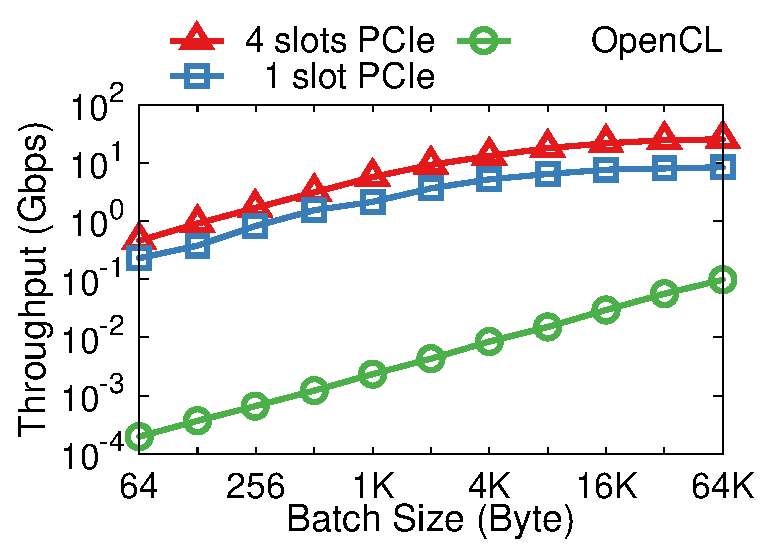
\includegraphics[width=0.225\textwidth]{eval/pcie_1}
	}
	\subfigure[]{
		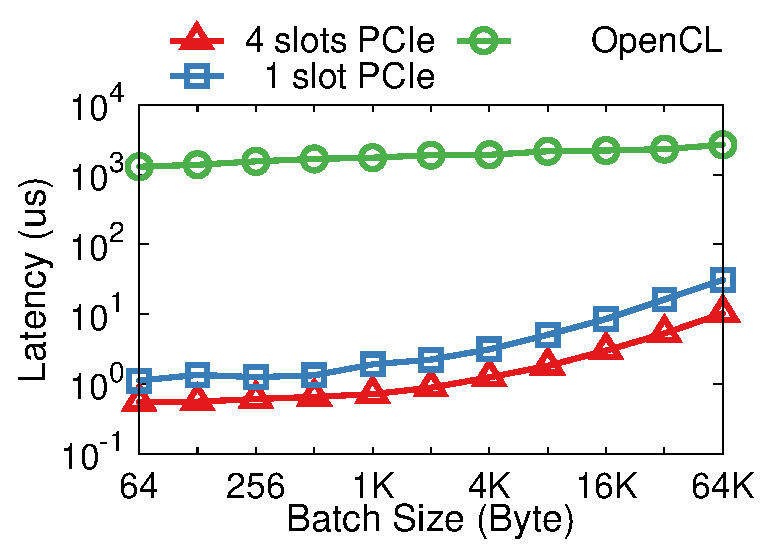
\includegraphics[width=0.225\textwidth]{eval/pcie_2}
	}
\vspace{-10pt}
	\caption{The performance of the PCIe I/O channel. The y-axis is in logarithmic scale. }
\vspace{-14pt}
	\label{fig:pcie}
\end{figure}

\egg{

\egg{
Control signals can only be generated by the manager thread. 
When the manager thread sends a signal to a target element in FPGA, it will embed the ID of the element in the signal message, and 
passes the message to \textit{CmdHub} through slot 32.
\textit{CmdHub} will parse the message and forward the signal request to corresponding elements, again through FIFO buffers. 
}



\egg{
As aforementioned, OpenCL advocates batch processing model where communication between host program and a kernel in FPGA must go through shared DRAM, and the host program cannot control the kernel while it is running.
We could use a special kernel to proxy messages between host program and the kernel via DRAM, but it incurs \approx1ms latency.
DDR access is performed via PCIe link and raw PCIe latency is merely \approx1$\mu$s. As we improve kernel communication efficiency with channels in place of shared memory, we design a host-kernel communication mechanism with channel abstraction for low latency and high throughput.
We leverage I/O channel in Altera OpenCL and AXI stream in Vivado HLS to connect the Catapult shell to kernels and built a PCIe bypass switch to arbitrate accesses for on-board DRAM and kernel I/O channel.

A PCIe link is split into multiple logically independent \textit{slots} which can operate in parallel.
One slot is reserved for signals. Remaining slots are assigned to channels between host and FPGA elements, so each channel can transfer data in parallel without head-of-line blocking.
On CPU side, each host element is run on a separate core and receives input flits via PCIe by polling or interrupt.
On FPGA side, each element that communicates with host is connected to an inbound demultiplexer and an outbound multiplexer, where load-adaptive batching is performed to improve peak throughput while preserving low latency under light load.
}

\egg{
With polling model, the latency of the PCIe I/O channel  is $< 2 \mu s$ when message size is small, but the latency will reach to $32 \mu s$
for full batched messages.
The interrupt model, however, will increase the latency.
}

\egg{
, where each slot is assigned to one CPU core. Our PCIe channel has two bottlenecks: (1) PCIe Gen2 x8 interface has 32 Gbps bandwidth, (2) PCIe data width is 128b and the clock frequency of Catapult shell is 200 MHz, which limits PCIe throughput to 25.6 Gbps. PCIe I/O channel offers 1\approx2$\mu$s RTT which translates to 400\approx800K host-kernel transactions per second. Polling mode yields lower latency and higher throughput, while interrupt mode latency can be improved by utilizing more cores and PCIe slots. Four CPU cores are sufficient to saturate maximum throughput for both polling and interrupt mode under 64KB batch size. Effectiveness of batching will be further evaluated in traffic dumper application.
}

}
%!TEX root=main.tex
\section{Applications}
\label{sec:application}

To evaluate the flexibility of \name, we have created five common NFs based on \name. 
All of them can run in our test-bed processing real-time traffic. 
%
Table~\ref{tab:applications} summarizes the number of elements included in each network function and the total LoC, including all elements specification and the cofiguration files.
%
Our experience also confirms the \name\ modular architecture greatly improves the code reuse and simplifies 
the construction of new NFs. 
As shown in Table~\ref{tab:elements}, there are many chances to reuse one element in many applications, \eg, L4\_Parser 
is used in all five NFs in this paper (A1-5).
%
Each NF may take 1\approx 2 weeks for one programmer to develop and debug. 
We find that the ability of joint CPU/FPGA processing would also greatly help 
debugging, as we can move 
an element in question to CPU, so that we can easily print logs to track the problem.

%In the following, we discuss these NFs in details.

\smalltitle{A1. Packet generator (PktGen) and capture (PktCap).} PktGen can generate various
traffic patterns based on different profiles. 
It can generate different sized flows and schedule them to start at different time, 
following given distributions. 
%
Generated flows can further pass through different traffic shapers to control the flow rates and their burstiness. 
PktCap simply redirects all packets it receives to \textit{logger} elements, which are usually located in the host.
Since a single logger cannot fully utilize the PCIe I/O channel capacity, PktCap has a Receive Side Scaling (RSS)
element in FPGA to distribute packets to multiple loggers based on the hash of flow 5-tuple.
%
Since our PCIe channel has less capacity than 40G NIC, we add an \textit{extractor} element that extracts only important
fields of a packet (\eg 5-tuple, DSCP and VLAN tag if any) and forwards these fields (total 16B), together with a timestamp
 (4B) to the logger element across PCIe.
%
PktCap is one example demonstrating the importance of joint CPU/FPGA processing. 
Compared to FPGA, CPU has 
more memory for buffering and can easily access other storages, \eg, HDD/SSD drives as in \cite{lee2015flosis}, and therefore it makes more sense to run loggers on CPU.

\smalltitle{A2. Openflow firewall (OFW).} Our Openflow~\cite{mckeown2008openflow} firewall supports 
both exact- and wildcard-matching of flows.
The exact-match table is implemented using Cuckoo Hashing~\cite{cuckoo} and contains 128K entries that match against flow 5-tuples. 
The wild-card match is based on TCAM.
However, a naive TCAM implementation with 512 104-bit entries takes 65\% logic resource of our FPGA.
Instead, we use BRAM-based TCAM~\cite{jiang2013scalable}. 
BRAM-based TCAM breaks search key into 8-bit keys and use them to address lookup tables, which trades memory for logic area. A BRAM TCAM with 2K entries takes 14\% logic and 43\% BRAM.
Additionally, we design a HashTCAM to leverage the fact that many entries in flow tables 
share the same bit-masks.
HashTCAM divides the table space into a number of smaller hash tables, each of which 
is associated with a bit-mask.
%
Any incoming packet will first perform an ``and'' operation before looking up the hash table.
Each entry in the table is also associated with a priority. 
An arbitrator logic is applied to  
select the matched entry with the highest priority. 
HashTCAM has better tradeoff between capability and area cost.
A HashTCAM with 16K flow entries and 16 distinct bit-masks (similar to Broadcom Trident II~\cite{broadcomethernet}) takes 19\% logic and 22\% BRAM.
%
The manager program always tries to group rules based on their bit-masks and places
groups with most rules into HashTCAM. 
%
The rest rules, which casnnot fit into any groups in HashTCAM, are then put into 
BRAM-based TCAM. 


\smalltitle{A3. IPSec gateway (IPSecGW).}
One issue with software NFs is that the CPU soon becomes a bottleneck when packets require some
computation intensive processing, \eg, IPSec~\cite{packetshader}.
%
We have built an IPSec datapath that is able to process IPSec packets with AES-256-CTR encryption and SHA-1 authentication. 
As shown in \S\ref{subsec:lib}, a single AES\_CTR element can achieve only 27.8~Gbps throughput. Therefore, we need two
AES\_CTR elements to run in parallel to achieve line rate.
SHA-1, however, is tricky. The SHA-1 divides a packet into smaller data blocks (64B). 
Although the computation in one data block can be pipelined, 
there is a dependency between successive blocks inside one IP packet -- the computation of the next block cannot start before the previous
block has finished! 
If we process these data blocks sequentially, the throughput would be as low as 1.07 Gbps. 
Fortunately, we can leverage parallelism among different packets. 
While the processing of a data block of the current packet is still going, we feed a data block of a different packet. 
Since these two data blocks do not have dependency, they can be processed in parallel. 
To implement this, we design a new element called \textit{reservo} (short for reservation station), which buffers up to 64 packets and schedules 
independent blocks to SHA-1 element. After the signature of one packet has been computed, the \textit{reservo} element will 
send it to a next element that appends SHA-1 HMAC to the packet.
%
There is one more tricky thing. 
Although SHA-1 element has a fixed latency, the overall latency of a packet is different, \ie, proportional to packet size. 
When multiple packets are scheduled in SHA-1 computation, these packets may be
out-of-order, \eg, a smaller packet behind a large packet may finish earlier.
%
To prevent this, we further design a \textit{reorder buffer} element after SHA-1 element
that stores the out-of-order packets and restore the original order
 according to sequence numbers of packets. 

\smalltitle{A4. L4 load balancer (L4LB).} We implement L4LB according to \textit{multiplexer} (MUX) in Ananta~\cite{ananta}.
%
The MUX server basically looks into the packet header and sees if a \textit{direct address} (DIP) has been assigned to the flow.
If so, the packet is forwarded to the server indicated by DIP via a NVGRE tunnel. Otherwise, the MUX server will call a local controller to
allocate a DIP for the flow.
%
\egg{Per-flow state is required in MUX server.
Hash-based ECMP cannot be used since there are failures and avoiding black holes requires changing backend server list on-the-fly. Further, advanced LB may also require load-aware 
balancing.}
%
A flow table is used to record the mapping of flows to their DIPs.
%
To handle the large traffic volume in datacenters, it requires the L4LB to support up to 32 million flows in the flow table.
Clearly, such a large flow table cannot fit into the BRAM of FPGA, and has to be stored in onboard DDR memory.
However, accessing DDR memory is slow. 
To improve performance, we create a 4-way associative flow cache in BRAM with 16K 
cache lines. The Least Recently Used (LRU) algorithm is used to replace entries 
in the flow cache.

In our implementation, an incoming packet first passes a \textit{parser} element 
which extracts the 5-tuple and sends them to the \textit{flow cache} element.
If the flow is not found in the flow cache, the packet's metadata is forwarded
to the global flow table, which reads the full table in DDR.
%
If there is still no matching entry, the packet is the first packet of a flow and 
a request is sent to an \textit{DIPAlloc} element to allocate a DIP for the flow 
according to load balancing policy.
After the DIP is determined, an entry is inserted into the flow table. 

After deciding the DIP of a packet, an encapsulation element will 
retrieve the next-hop information, \eg, IP address and VNET ID, and 
generate a NVGRE encapsulated packet accordingly. 
%
%For remaining packets of the flow, DIP is extracted from flow state.
A flow entry would be invalidated if a FIN packet is received, or a timeout occurs
before receiving any new packets from the flow.
%After DIP is determined, we retrieve next-hop metadata from BRAM and encapsulate an NVGRE header to direct the packet to assigned DIP.

We put all elements in FPGA except for the \textit{DIPAlloc} element.
Since only the first packet of a flow may hit \textit{DIPAlloc} and the allocation policy also could be complex, it is more suitable to run 
\textit{DIPAlloc} on CPU, being another example of joint CPU-FPGA processing.
%
\egg{
To handle the large traffic volume in datacenters, it requires the L4LB to support up to 32 million flows in the flow table.
Clearly, such a large flow table cannot fit into the BRAM of FPGA, and has to be stored in onboard DDR memory.
Accessing DDR memory is slow. To improve performance, we further create a 4-way associative flow cache in BRAM with 16K 
cache lines. The flow cache is replaced based on the Least Recently Used (LRU) algorithm.
DDR memory access is a fat pipeline stage as shown in Figure \ref{fig:unbalance}. We move the DDR access part to a separate element to make the fast path run asynchronously with slow path.}

\smalltitle{A5. pFabric flow scheduler.} As the last application, we use \name\ to implement one recently proposed packet
scheduling discipline -- pFabric~\cite{pfabric}. 
pFabric scheduling is simple. It keeps only a shallow buffer (32 packets), and always dequeues the
packet with the highest priority. When the buffer is full, the packet with the lowest priority is dropped.
%
pFabric is shown to achieve near-optimal flow completion time in datacenters. 
%
In the original paper, the authors proposed using a binary comparison tree (BCT) to select the packet with the highest priority. 
However, while BCT takes only $O(log_2N)$ cycles to compute the highest priority packet, there is a dependency between 
successive selection processes. It is because only when the previous selection finishes can we know the highest priority packet, and
then the next selection process can be started reliably.
This limitation would require the clock frequency to be at least 300MHz to achieve the line rate of 40Gbps, 
which is not possible for our current FPGA platform.
%
In this paper, we use a different way to implement pFabric scheduler which is much easier to  parallelize. 
The scheme is based on \textit{shift register priority queue}~\cite{moon2000scalable}.
Entries are kept in a line of $K$ registers in non-increasing priority order.
When dequeuing, all entries are shifted right and the head is popped. This takes just 1 cycle.
For an enqueue operation, the metadata of a new packet is forwarded to all entries.
And now, with each entry, a local comparison can be performed among 
the packet in the entry, the new packet, and the packet in the neighboring entry. 
Since all local comparisons can be carried in parallel, the enqueue operation can 
also finish in 1 cycle.
Enqueue and dequeue operations can further be parallelized. 
Therefore, a packet can be processed in one cycle.


\egg{
pFabric \cite{alizadeh2013pfabric} is a near-optimal datacenter transport based on priority scheduling and dropping. Packets are scheduled based on its flow size or remaining flow size in a small queue. Our pFabric scheduler implementation (Figure \ref{fig:PFabric}) support 4-giga strict priorities, including a PriorityQueue which deques the packet with highest priority and drops overflow packets with lowest priority, a ReorderQueue to find the earliest packet from the flow with highest priority to avoid starvation and keep packet ordering, and a PacketBuffer to receive packets into buffer and schedule or drop packets out of buffer. Since queue size in a perfectly load balanced fabric should be small, we choose shift register priority queue for maximum throughput and clock frequency.

ReorderQueue is another shift register queue ordered by flow hash. On enque command from PacketBuffer, packet metadata with flow hash $f_{new}$ is enqued to entry $i$ where $f_{i-1} < f_{new} \leq f_{i}$. On deque command from PriorityQueue, the entry $i$ with $f_{i} = f_{deque} < f_{i+1}$ is dequed. Packets with a same flow hash are dequed in the same order as they are enqued.


\begin{figure}[h!]
	\centering
	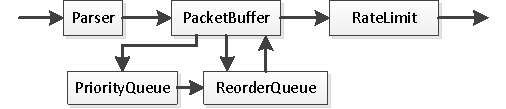
\includegraphics[width=1.0\columnwidth]{image/PFabric}
	\vspace{-0.30in}
	\caption{PFabric Element Graph}
	\vspace{-0.10in}
	\label{fig:PFabric}
	%    \vspace{-2mm}
\end{figure}
}

%%!TEX root=main.tex
\section{ClickNP Language}
\label{sec:language}

\subsection{Element Graph}

ClickNP script defines a directed graph of elements and channels, which adapts some syntax from the Click modular router \cite{kohler2000click}.

Following ClickNP script and figure \ref{fig:ClickNPScriptExample} defines the NIC-to-ToR part of a network application with NVGRE encapsulation and Per-VM rate limiting.

\begin{figure}[!t]
	\centering
	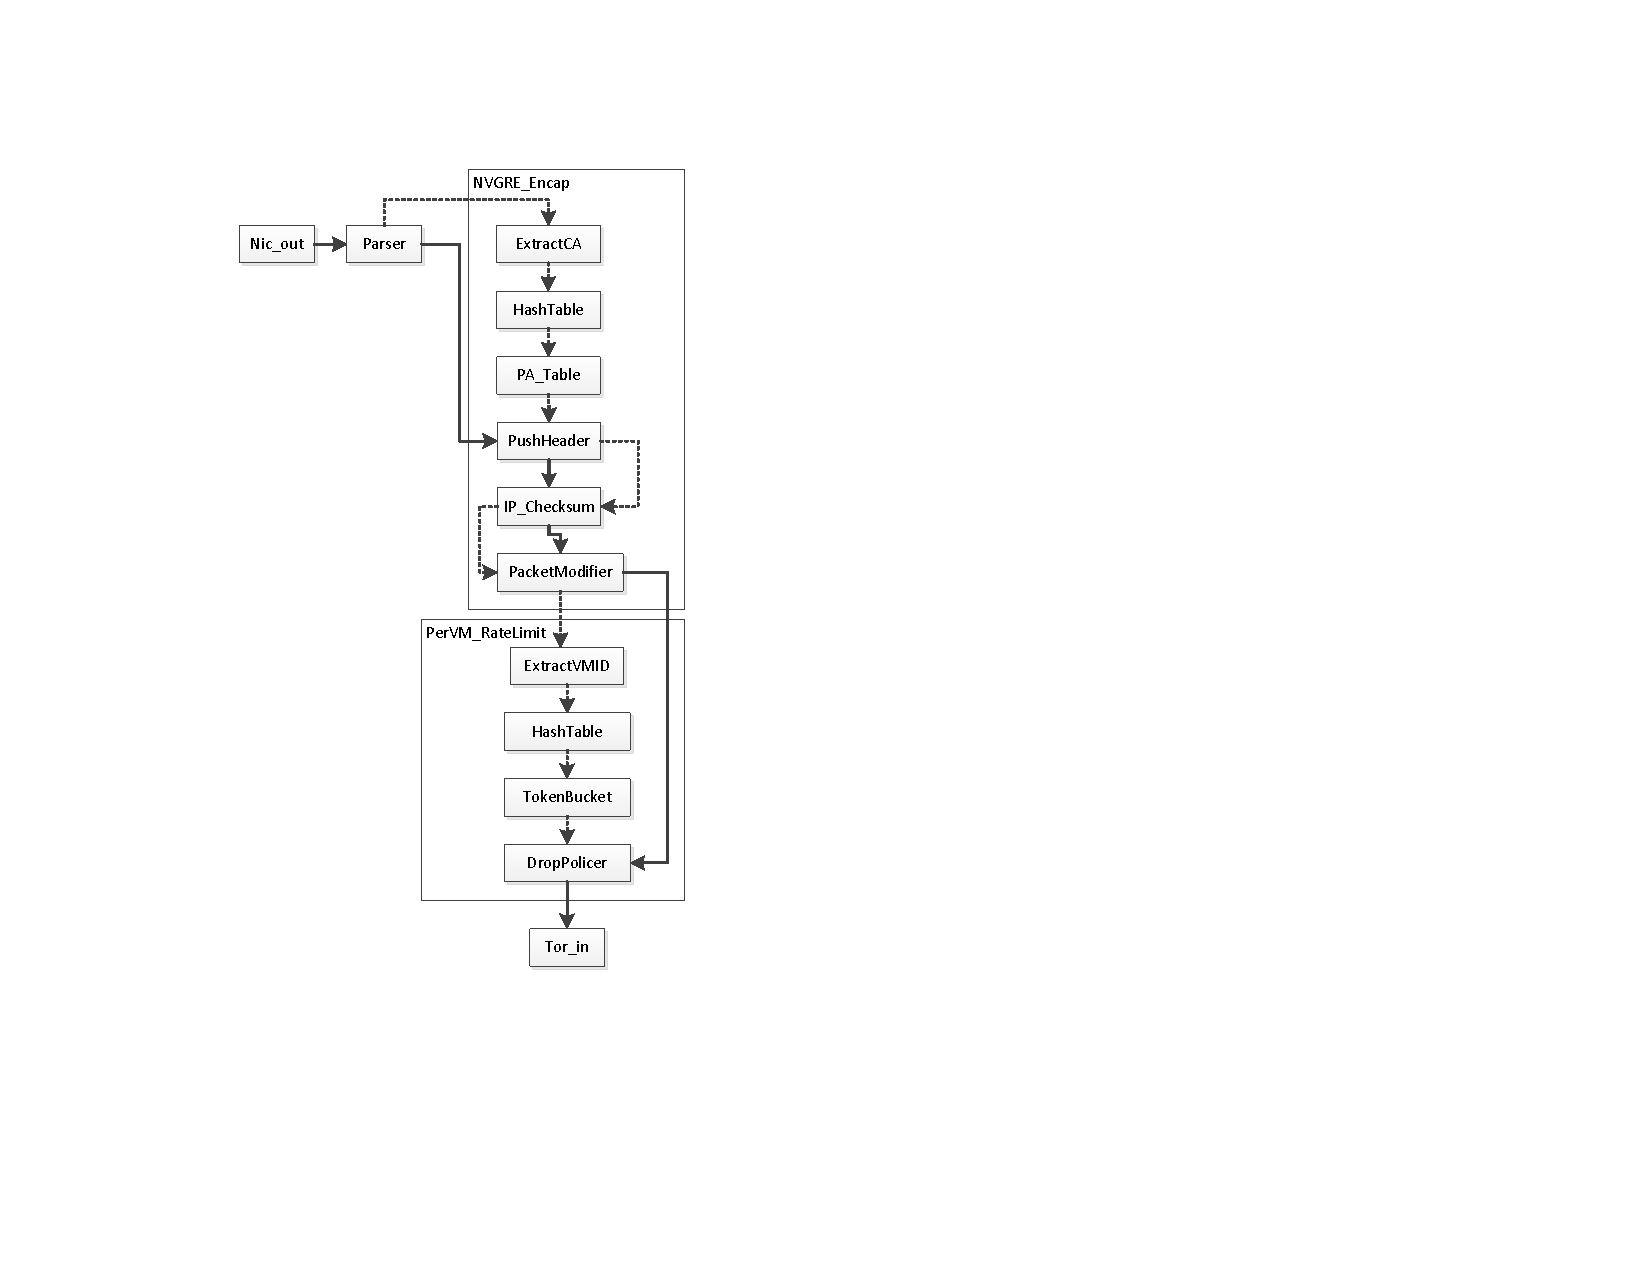
\includegraphics[width=1.0\columnwidth]{image/ApplicationExample}
	\vspace{-0.25in}
	\caption{NVGRE Encap + Rate Limiting in ClickNP}
	\vspace{-0.15in}
	\label{fig:ClickNPScriptExample}
	%    \vspace{-2mm}
\end{figure}

\begin{lstlisting}
.element_group NVGRE_Encap {
    PushHeader :: encap (2,2)
    begin[1] -> [1]encap -> IP_Checksum (2,2) -> PacketModifer (2,2) -> end
    begin[2] -> ExtractCA (1,1) -> HashTable @ (1,1,14) -> PA_Table @ (1,1) -> [2]encap
}
.element_group PerVM_RateLimit {
    DropPolicer :: action (2,2)
    begin[1] -> [1]action -> end
    begin[2] -> ExtractVMID (1,1) -> HashTable @ (1,1,4) -> TokenBucket @ (1,1) -> [1]action
}
PerVM_RateLimit :: ratelimit (2,2)
nic_out -> Parser (1,2) -> NVGRE_Encap (2,2) -> ratelimit[1] -> tor_in
ratelimit[2] -> Drop (1,0)
\end{lstlisting}

Per clock cycle, each element can read at most one 64-byte message from each input channel and write zero or one 64-byte message to each output channel. A channel either pass \textit{flit} messages (solid line) or \textit{metadata} messages (dotted line). Each flit contains 32 bytes of packet content and flags indicating start of packet (sop) and end of packet (eop). Metadata format is user-defined, containing parsed packet header and optionally a subsequent action.

Lines 1--5 defines an \textit{element group} of 6 elements. Line 2 instantiates a \textit{PushHeader} element with name \textit{encap}. Numbers in parentheses stand for number of input and output ports, and optional subsequent numbers are element parameters (see section \ref{subsec:elementdef}). Square brackets indicate the port number to be connected via channel. ``@'' symbol indicates on-the-fly host control.

Metadata containing parsed packet headers flow into the element group via port 1, where Customer Address (CA) is extracted and matched against a \textit{HashTable} controlled by host problem, then the match result is used as the index to Physical Address (PA) table (also controlled by host program). PA table modifies the action part of metadata to contain outer header offset, length and data. Along with packet content flits buffered in channel, metadata is sent to \textit{PushHeader} element where packets actually get shifted. The metadata (with action cleared) and packet flits continue to the \textit{IP\_Checksum} element where new IP header checksum is calculated and a packet modify action is generated to update the IP checksum field in subsequent \textit{PacketModifier} element.

Our initiative for separating flit and metadata messages is not only for clarity but also for performance. One reason is to alleviate the throughput burden of lookup tables. Typically table lookup is done once per packet, while each Ethernet packet has 2--48 flits. If flits are passed through via lookup tables, since we can process at most one flit per cycle, we need to finish each iteration in one cycle in order to reach line rate, but lookup tables which both read and write to local memory need two cycles due to memory timing.

Another reason for flit-metadata separation is to pipeline packet modification actions. For example, in \textit{IP\_Checksum} action, the IP header crosses the boundary of first and second flits, therefore the checksum can only be calculated after the first two flits have arrived. However, the IP checksum field to be updated is in the first flit. If we use one channel for both flit and metadata, then the element has to output nothing in the first cycle processing a packet. As discussed in section \ref{subsec:designgoals}, such per-packet idle cycle is unacceptable for our line-rate FPGA implementation. By transferring flit and metadata in separate channels, \textit{IP\_Checksum} element can pass through flits while calculating the checksum, and flits are buffered in the channel between \textit{IP\_Checksum} and \textit{PacketModifier}. When metadata containing IP checksum is received by \textit{PacketModifier}, the first flit is also ready. This coding style eliminates the need for buffers within elements which are more resource hungry than buffers within channels.

A network application is typically built with a parser and a chain of network functions. A network function first builds a lookup key from parsed packet header, match the key in a lookup table (section \ref{subsec:lookuptables}), then builds an action based on the match result. The action and packet flits are then passed into an action element. This coding convention allows lookup table elements to be generic, actions to be chained, network functions to be chained and packet parser to be shared.

\subsection{Element Definition}
\label{subsec:elementdef}

An element has five components: states, ports, an initializer, a data handler and a signal handler.

\textit{States} define variables that are persistent throughout the lifecycle of an element. Each element has some input and output \textit{ports}, whose number is configured by element graph. \textit{Initializer} is executed once right after the element launches. Main processing loop is composed of a data handler (\textit{.handler}) and a signal handler (\textit{.signal}).

Each element instance with host control enabled (``@'' symbol) will be connected to two special kernels \textit{CmdHub\_in} and \textit{CmdHub\_out}. \textit{CmdHub\_in} is a demux from PCIe input to signal-enabled kernels, \textit{CmdHub\_out} is a mux from signal-enabled kernels to PCIe output. For each iteration, if there is signal input from the host program, the signal will be unmarshaled from PCIe packet to \textit{event}, the signal handler is called, then \textit{outevent} is marshaled to a PCIe packet and sent back to host. Otherwise, input channels are checked for new message, the data handler is called, then output channels are written.

Data handler should check whether or not its input ports have message ready, read states, perform calculation, write back changes to states, optionally write to output ports and return which input ports are to read next iteration. Each input port have a buffer of one message size, and a handler is free to consume or not consume the message by calling or not calling \textit{clear\_input\_ready}. If there are multiple calls to \textit{set\_output\_port} for a same port in one iteration, only the last call will be effective.

The \textit{IP\_Lookup} element below is a binary-tree based IP classifier. The number of nodes per tree level is controlled by the third parameter in element instantiation. The element reads IP address from input port 1, consults the table and writes result to output port 1.

To reduce resource utilization in FPGA, the host program should keep an exact copy of the tree structure, and the assignment of nodes for rule update is handled by host program. The signal handler executes node update instructions from host program. The read interface in signal handler is for crash recovery of host program, so that the restarted host program can rebuild the tree from FPGA.

\begin{lstlisting}
.element IP_Lookup {
    .state {
        // levels of binary tree
        constexpr DEPTH = 32;
        // max entry num per level
        constexpr WIDTH = $3;
        .repeat (depth, 0, DEPTH) {
            constexpr w = ((1<<depth) < WIDTH ? (1<<depth) : WIDTH);
            short value$depth[w];
            short left$depth[w];
            short right$depth[w];
        }
    }
    .init { }
    .handler {
        if ( !input_ready(PORT_1) )
            return PORT_1;
        bool *ip = (bool *) &input_data[1];
        clear_input_ready(PORT_1);

        short pos = 0;
        short result = 0;
        .repeat (depth, 0, DEPTH) {
            result = value$depth[pos];
            if (ip[depth])
                pos = left$depth[pos];
            else
                pos = right$depth[pos];
            if (pos == 0)
                BREAK;
        }
        set_port_output(1, result);
        return PORT_1;
    }
    .signal (uchar cmd, uchar depth, uint pos, uint value, uint left, uint right) {
        uint pos = event.pos;
        .repeat (i, 0, DEPTH) {
          if (i == event.depth)
            switch (event.cmd) {
              case 1: // update
              value$i[pos] = event.value;
              left$i[pos]  = event.left;
              right$i[pos] = event.right;
              break;
              case 2: // read
              outevent.value = value$i[pos];
              outevent.left  = left$i[pos];
              outevent.right = right$i[pos];
              break;
            }
        }
    }
}
\end{lstlisting}

\textit{.repeat (depth, 0, DEPTH)} generates \textit{DEPTH} copies of code with string \textit{\$depth} replaced with 0, 1, 2\ldots \textit{DEPTH}-1. \textit{BREAK} is a special statement to jump to the end of repeated code blocks. Following show the storage regions for variables.

\begin{itemize}
	%\item \textit{counter} is compiled to a register, which is read and written at most once per iteration, and can be done in one cycle.
	%\item \textit{state\_reg} is compiled to an array of registers because all accesses to the array have constant index, after the loop is unrolled. Each register in the array is read and written once per iteration, and also can be done in one cycle.
	\item State arrays \textit{value}n, \textit{left}n and \textit{right}n are compiled to (3 * \textit{DEPTH}) SRAM blocks. Each array is read (in handler) or written (in signal) once per iteration, so the element can be fully pipelined.
	%\item \textit{Param} is a pointer to global memory. Access to global memory is the bottleneck of the while loop.
	\item Local variables \textit{ip}, \textit{pos} and \textit{result} are intermediate variables in the combinational logic and will occupy no storage space on FPGA.
	\item Loop control variables \textit{depth} and \textit{i}, as well as \textit{constexpr}s, are syntactic sugar for code generation.
\end{itemize}

The tree lookup logic in lines 23--31 is automatically pipelined by ClickNP toolchain. After data flow analysis, variables \textit{pos} and \textit{result} are each split into multiple variables in single static assignment (SSA) form. Since SRAM read has one cycle latency, the lookup will take at least \textit{DEPTH} cycles. Fortunately, these memory read operations can be pipelined. A pipeline with \textit{DEPTH} stages is inferred, each stage holds a copy of live variables \textit{ip}, \textit{pos} and \textit{result} in registers. Different stages of the pipeline processes different copies of live variables (i.e. different copies of input data) simultaneously. Pipelining improves throughput by exploiting temporal parallelism.

The tree update logic in lines 41--43 are independent, so the three memory writes are performed in parallel, which improves throughput by exploiting spatial parallelism.

\subsection{Host Communications}

Signal handler is a stop-and-wait mechanism for host-to-kernel communication. Kernels also need to initiate communications, for example to send alerts, dump packets and use host memory as cache. We develop a streaming interface for kernels to communicate with host program via channels as if host program was another kernel. To use the streaming host interface, an element connects to \textit{host\_in} pseudo-element for input and \textit{host\_out} for output.

ClickNP compiler generates a C++ class for each element type, including 5 methods:
\begin{itemize}
	\item \textit{launch}, launches the corresponding kernel.
	\item \textit{signal}, marshals parameters, send an event to the signal handler, wait to receive outevent and unmarshals the response.
	\item \textit{send}, send a message to kernel via streaming interface.
	\item \textit{receive}, receive a message (block or non-block) to kernel via streaming interface.
	\item \textit{setCallback}, if set, the callback function will be called every time a message is received via streaming interface.
\end{itemize}

The C++ class can be extended to add more methods with clearer semantics. For example, \textit{IP\_Lookup} class provides methods \textit{addRule}, \textit{deleteRule}, \textit{clearTable} and \textit{reloadTable} to encapsulate internal states of the IP lookup tree and a series of node update operations needed for one rule update.

All element classes share a common base class \textit{Element}, and ClickNP compiler generates a \textit{std::map} of element names and element class instances. A host program should first initialize the platform, then execute the \textit{launch} method of each element object.
%%!TEX root=main.tex
\section{ClickNP Elements}
\label{sec:elements}

In this section we show LOC (Line Of Code) (excluding host program) and resource utilization of some common elements under reasonable parameter settings.

All elements shown in this section can process 40 Gbps line rate for all Ethernet packet sizes under 190 MHz clock rate, i.e. one cycle per iteration for elements processing packet flits, and up to 3 cycles per iteration for elements processing metadata only.

\subsection{Basic Connectors}

\begin{table}[h!]
	\centering
	\label{tab:Basic Connectors}
	\begin{tabular}{l|r|r|r}
		Element & LOC & Logic & Memory \\
		\hline
		Tee	&  & \%  & 0\% \\
		Mux	&  & \% & 0\% \\
		Demux & & \% & 0\% \\
		FlitMux & & \% & 0\% \\
		FlitDemux & & \% & 0\% \\
	\end{tabular}
\end{table}


\subsection{Programmable Header Parser}

Packet parser is an important part of network processor, whose complexity comes from tunneling protocols and diversity of protocols in each layer.

The uncertainty of outer layers introduce non-constant header offset in the packet. For example, an Ethernet packet without VLAN has IP header offset 14, an Ethernet packet with VLAN has IP header offset 18. Simply using a variable as index to packet byte array is very ineffective in OpenCL. An array with one or more variable index access will be implemented as block SRAM in FPGA, which only support one read operation per cycle. In order to parse the packet header (which includes many array accesses) in one cycle, we need to implement the packet buffer as register in FPGA, which requires all accesses to the packet buffer array to have constant index.

%If we create an element for each packet header, then each element needs to shift the packet payload in order to ``peel off'' the parsed header. The first drawback is that each element introduces some overhead in logic utilization. Since there are multiple leaf elements representing the innermost header to parse, and different elements have different latencies, output packets at the final mux will be out-of-order. The reordering buffer would take considerable local memory. Furthermore, in the case of network virtualization and tunneled protocols, there will be a loop of elements that each tunneled packet would travel twice, which lowers throughput of packet parser.

To implement a packet parser with all packet buffer offsets to be constant, without shifting packet payload after each header is parsed, we need to enumerate all possible parsing paths (e.g. Ethernet $\rightarrow$ IP, Ethernet $\rightarrow$ VLAN $\rightarrow$ IP), duplicate parser code for each path and calculate offset for each access to packet buffer. Doing such work manually is frustrating and error-prone, therefore ClickNP provides a general \textit{.state\_machine} abstraction, which can generate a decision tree composed of all possible state migration paths and calculate all packet buffer offsets at compilation time.

\begin{lstlisting}
.state_machine {
    constexpr offset = 0;
    .parser_define MAX_STATE_REPEAT 2;
    begin {
        constexpr offset += 12;
        ushort next_proto = *(ushort *) &input[offset];
        constexpr offset += 2;
        if (next_proto == PROTO_VLAN)
            .goto_state VLAN;
        else if (next_proto == PROTO_IPv4)
            .goto_state IPv4;
        else
            .goto_state end;
    }
    VLAN {
        if (!meta.vlan)
            meta.vlan = *(ushort *) input[offset];
        ushort next_proto = *(ushort *) &input[offset + 2];
        constexpr offset += 4;
        if (next_proto == 0x8100)
            .goto_state VLAN;
        else if (next_proto == 0x0800)
            .goto_state IPv4;
        else
            .goto_state end;
    }
    IPv4 {
        .if (STATE_REPEAT == 1) {
            meta.src_ip = *(uint *) &input[offset + 12];
            meta.dst_ip = *(uint *) &input[offset + 16];
        } .else {
            meta.inner_src_ip = *(uint *) &input[offset + 12];
            meta.inner_dst_ip = *(uint *) &input[offset + 16];
        }
        ushort next_proto = input[offset + 9];
        constexpr offset += 20;
        if (next_proto == 94)
            .goto_state IPv4; // IP-in-IP
        else if (next_proto == 97)
            .goto_state begin; // ETHERIP
        else
            .goto_state end;
    }
}
\end{lstlisting}


\begin{figure}[!t]
	\centering
	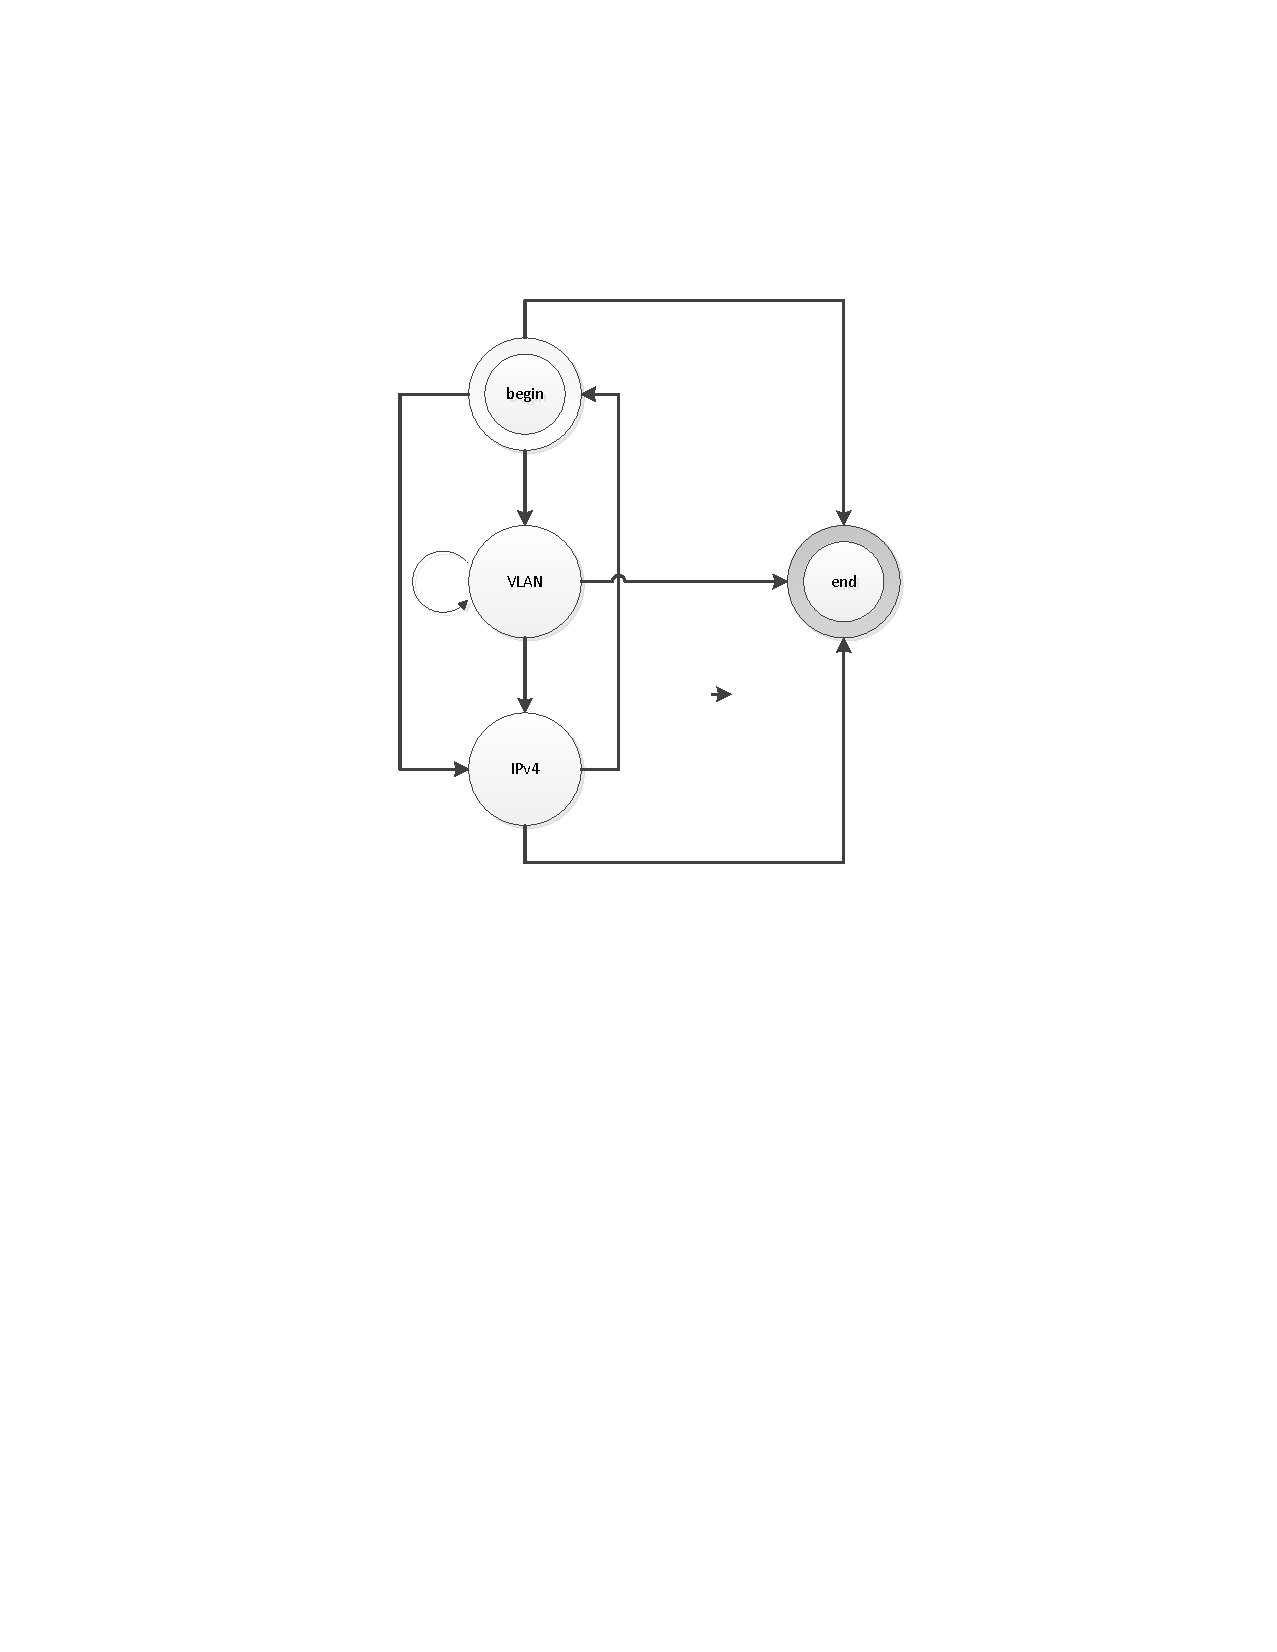
\includegraphics[width=0.7\columnwidth]{image/StateMachine}
	\vspace{-0.15in}
	\caption{Sample State Machine for Header Parser}
	\vspace{-0.15in}
	\label{fig:StateMachine}
	%    \vspace{-2mm}
\end{figure}

Above code implement a sample header parser in figure \ref{fig:StateMachine}, each state is set to repeat at most twice. 44 lines of code with 3 states generates 314 lines of code with 27 states, which takes 2\% logic resource.

Following show some parsers to extract metadata from some well-known protocols. The element code can be easily modified to extract new fields or incorporate new protocols.

\begin{table}[h!]
	\centering
	\label{tab:PacketParsers}
	\begin{tabular}{l|r|r|r}
		Element & LOC & Logic & Memory \\
		\hline
		EthVlanParser & & \% & \% \\
		IPv4\_Parser & & \% & \% \\
		IPv6\_Parser & & \% & \% \\
		FlowTuple\_Parser & & \% & \% \\
		TCP\_Parser & & \% & \% \\
		NVGRE\_Parser & & \% & \% \\
		VXLAN\_Parser & & \% & \% \\
	\end{tabular}
\end{table}

\subsection{Lookup Tables}
\label{subsec:lookuptables}

\textit{HashTable} is implemented using Cuckoo hash \cite{pagh2004cuckoo} with two memory banks, which can be used for exact matching.

\begin{figure}[h!]
	\centering
	
\includegraphics[width=0.6\columnwidth]{image/logo}
	\vspace{-0.15in}
	\caption{HashTable Collision Rate, x: occupancy, y: hash collision rate, lines: sequential IP, sequential port, random, theory}
	\vspace{-0.15in}
	\label{fig:HashTableCollisionRate}
	%    \vspace{-2mm}
\end{figure}

\textit{TCAM} compares all entries in parallel and finds the lowest entry index that matches. Due to high logic resource utilization of TCAMs, we design \textit{HashTCAM} to trade off logic with memory. The design bases on an observation that bit-mask patterns in a set of real-world wildcard rules are limited. In order to reduce bit width of match key, commodity switching chips require users to specify bit-mask patterns prior to rule insertion, e.g. Broadcom Trident II \cite{broadcomethernet} only supports 16 bit-mask patterns.

HashTCAM also imposes a limitation on number of bit-mask patterns. For each unique bit-mask pattern, HashTCAM allocates a HashTable and fills its mask field. All rules sharing this bit-mask pattern can be inserted into HashTable whose key is masked original key and value is the index in original TCAM. Match results from HashTables are arbitrated to find the lowest index (highest priority) and get match result by index from SRAM. The \textit{HashTCAM} class in host program provides TCAM-like interface to abstract away HashTable allocation, rule update and SRAM update.

\begin{figure}[h!]
	\centering
	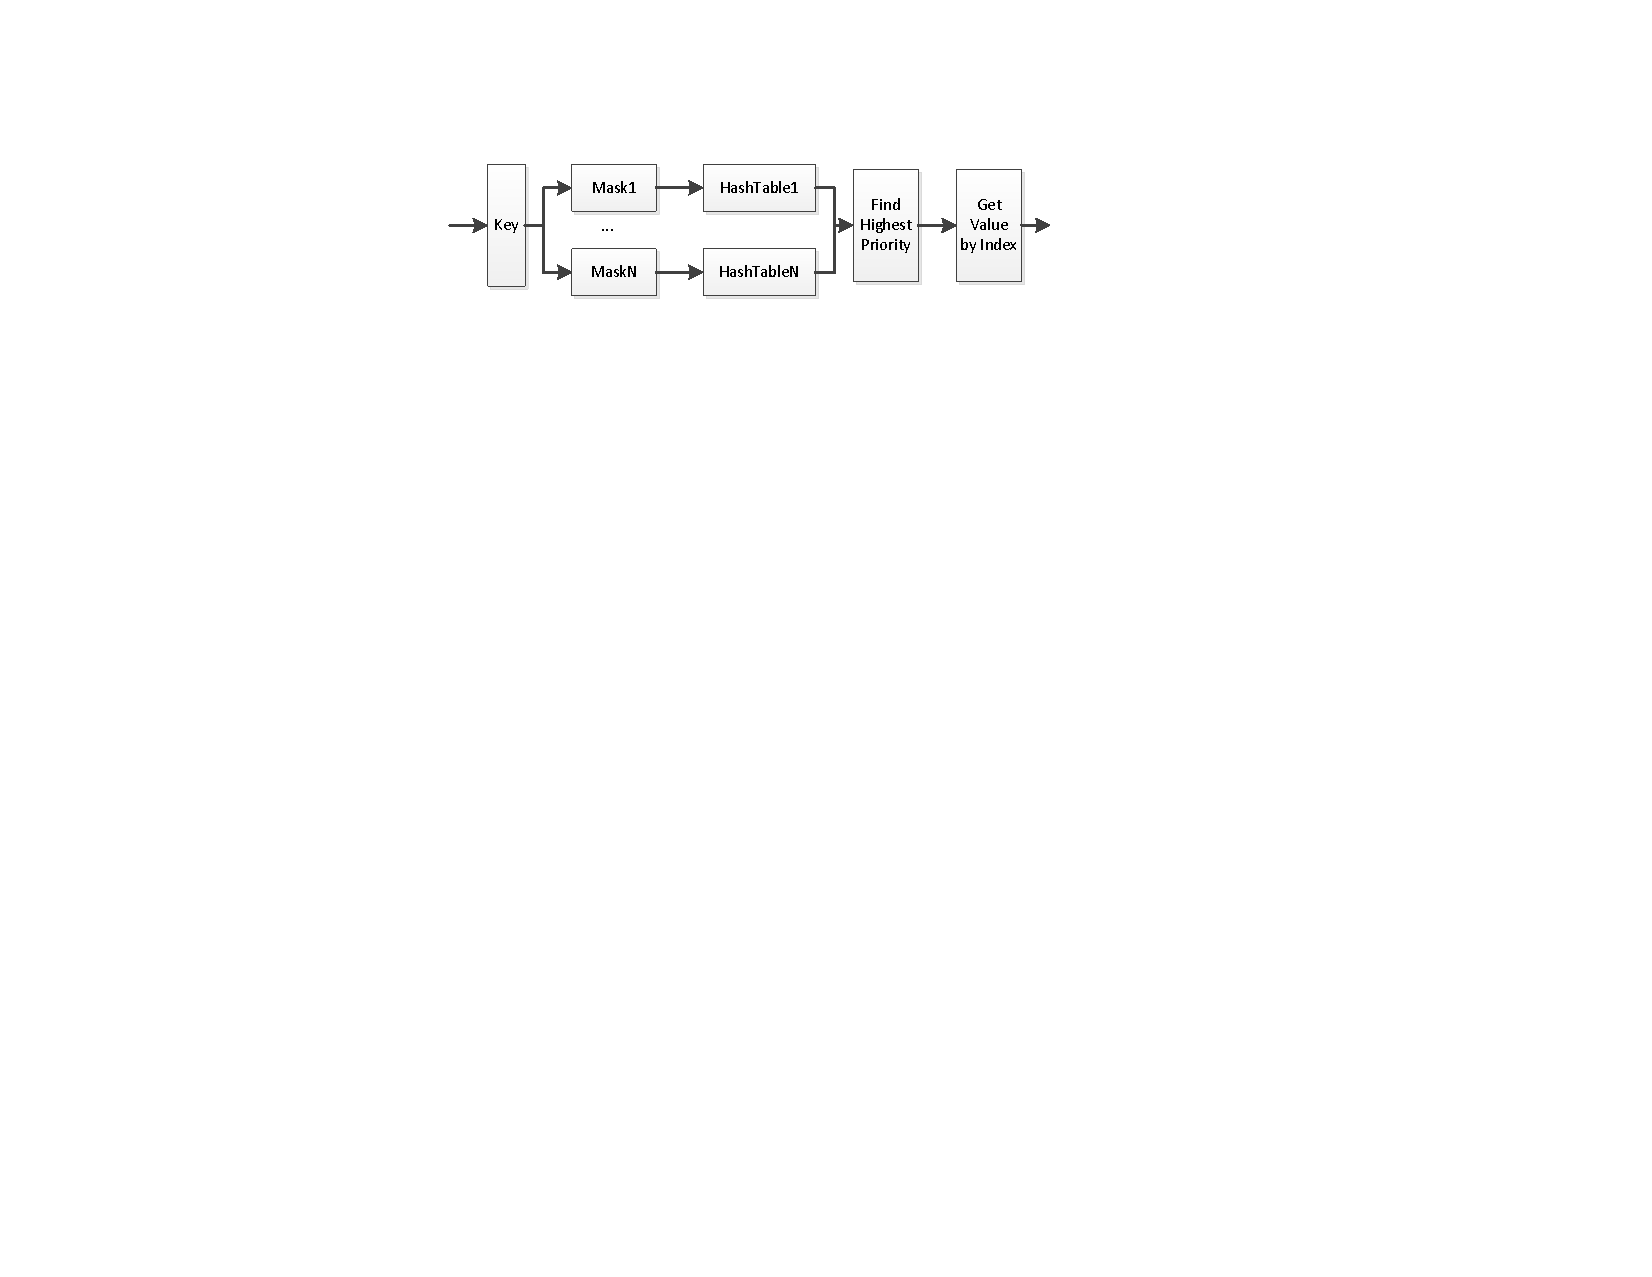
\includegraphics[width=1.0\columnwidth]{image/HashTCAM}
	\vspace{-0.30in}
	\caption{HashTCAM Architecture}
	\vspace{-0.10in}
	\label{fig:HashTCAM}
	%    \vspace{-2mm}
\end{figure}

Longest Prefix Match (\textit{LPM}) is essentially the \textit{IP\_Lookup} example in section \ref{subsec:elementdef}.

HashTable, TCAM, HashTCAM and LPM tables all match metadata, while deep packet inspection requires matching packet content. Content matching is much more resource hungry than matching a fixed offset in packet. \textit{StringMatch} works by comparing all offsets of a flit with the pattern byte-by-byte in parallel. \textit{RegexMatch} compiles multiple regexes into one NFA (nondeterministic finite automaton) and build a 32-level pipeline to process next byte and update NFA's active states every stage, similar to the \textit{IP\_Lookup} example. Due to logic resource constraint, current implementation of \textit{RegexMatch} compiles the NFA into FPGA image and does not allow on-the-fly regex reconfiguration.

\begin{table}[h!]
	\centering
	\label{tab:LookupTables}
	\begin{tabular}{l|r|r|r|r|r}
		Element & LOC & Key width & Size & Logic & Memory \\
		\hline
		HashTable 	& & 104b & 32K 	& 5\%  & 10\% \\
		TCAM 		& & 104b & 64	& 20\% & 0\% \\
		HashTCAM 	& & 104b & 16K    & 10\% & 10\% \\
		LPM			& & 32b  & 16K    & 10\% & 10\% \\
		StringMatch & & 32B  & 100	& & \\
		RegexMatch  & & 32B  & 100  & & \\
	\end{tabular}
\end{table}

Most signal handlers take only several cycles, so the update rate for lookup tables is bounded by the latency of PCIe channel: 120K updates per second in interrupt mode and 500K updates per second in polling mode.

\subsection{Packet Modifications}

\begin{table}[h!]
	\centering
	\label{tab:PacketModElements}
	\begin{tabular}{l|r|r|r}
		Element & LOC & Logic & Memory \\
		\hline
		PacketModifier 	& & \% & 0\% \\
		PushHeader		& & \% & 0\% \\
		PopHeader		& & \% & 0\% \\
		DropPolicer 	& & \% & \% \\
	\end{tabular}
\end{table}

\subsection{Traffic Schedulers}

\begin{table}[h!]
	\centering
	\label{tab:TrafficSchedulers}
	\begin{tabular}{l|r|r|r}
		Element & LOC & Logic & Memory \\
		\hline
		GenericPriorityQueue 	& & \% & 0\% \\
		RoundRobin		& & \% & 0\% \\
		WeightRoundRobin		& & \% & 0\% \\
		StrictPriority		& & \% & 0\% \\
		TokenBucket 	& & \% & \% \\
	\end{tabular}
\end{table}

%!TEX root=main.tex
\section{Evaluation}
\label{sec:eval}

\subsection{Testbed and methodology}

We evaluate \name\ in a testbed of 16 Dell R720 servers (\S\ref{subsec:sysarch}).
For each FPGA board, both Ethernet ports are connected to a Top-of-Rack (ToR) Dell S6000 switch~\cite{dells6000}.
All \name\ NFs are running on a Windows Server 2012 R2.
%
We compare \name\ with other state-of-the-art software NFs. 
For those NFs running on Linux, we use CentOS 7.2 with kernel version 3.10.
% delay measurement
In our test, we use PktGen to generate testing traffic at different rates 
with various packet sizes (up to 56.4~Mpps with 64B packets).
%
To measure the NF processing latency, we embed a generation timestamp in every testing packet.
When packets pass the NF, they are looped back to a PktCap which is located with PktGen 
in the same FPGA. 
%
Then we can determine the latency by subtracting the generation timestamp from the receiving 
time of the packet. 
%
The delay induced by the PktGen and PktCap was pre-calibrated via direct loop-back (without NFs) and removed from our data.

\egg{
To measure NF processing latency, we forward packets to an \textit{Echo} server using the second port. 
The Echo server runs an \textit{Echo} function in its FPGA, which simply bounces all packets back to the source. 
%
Then, we can compare the difference between the timestamps of a packet 
when it first arrives and when the processed packet is bounced back, to obtain the latency 
with nanosecond accuracy.
%
The delay induced by the Echo server was pre-calibrated and removed from our data.
In our test, we use PktGen to generate testing traffic, which can 
generate packets at up to 56.4 Mpps (64B packets).
}

\egg{
Ethernet ports of FPGAs and servers are connected to a Dell S6000 40GbE switch 
FPGAs are installed on Windows Server 2012 R2.
CPU-based benchmarks are performed on 

We use TrafficGen application to benchmark throughput and latency.
TrafficGen application generates a given traffic pattern or replays a trace, embeds timestamp in packet payload and sends to tor\_out.
Applications forward packets from tor\_in to nic\_out. When TrafficGen receives packet from nic\_in, the timestamp is extracted from payload to measure latency.
The wire loopback RTT of TrafficGen is 0.85$\mu$s for 64B packets and 1.39$\mu$s for 1504B packets, which is the system error in all latency numbers we present.
}

\begin{figure*}[t!]
	\centering
	\begin{minipage}{.6\textwidth}
		\centering
		\subfigure[]{
			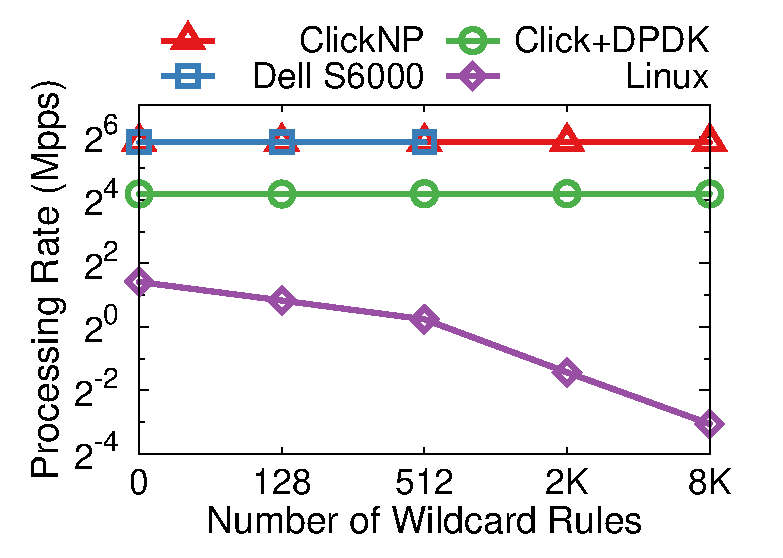
\includegraphics[width=0.45\textwidth]{eval/fw_1}
		}
	%	\subfigure[]{
	%		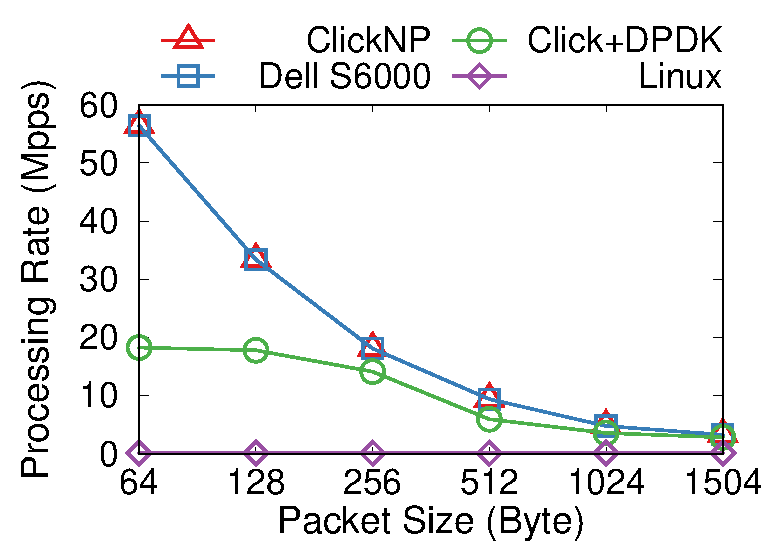
\includegraphics[width=0.225\textwidth]{eval/fw_2}
	%	}
		\subfigure[]{
			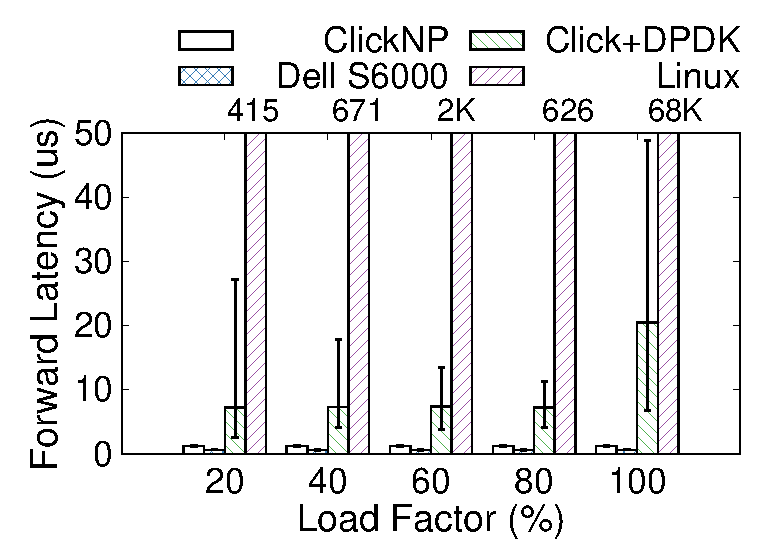
\includegraphics[width=0.45\textwidth]{eval/fw_3}
		}
		\subfigure[]{
			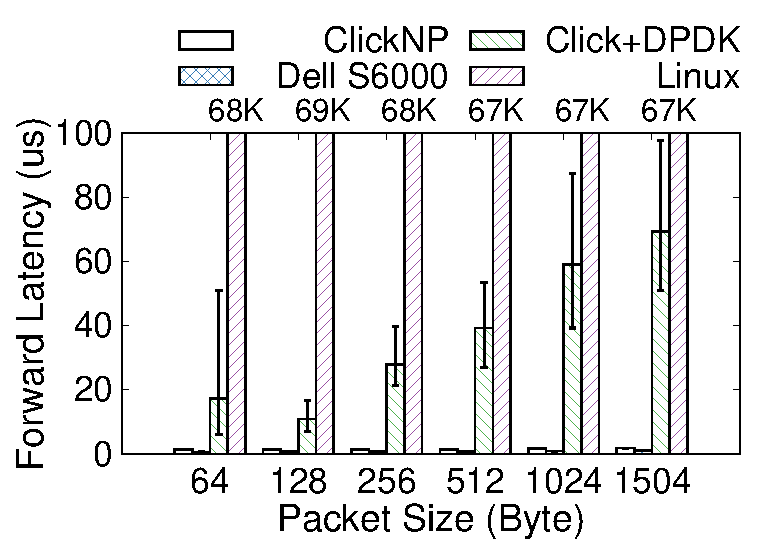
\includegraphics[width=0.45\textwidth]{eval/fw_4}
		}
		\subfigure[]{
			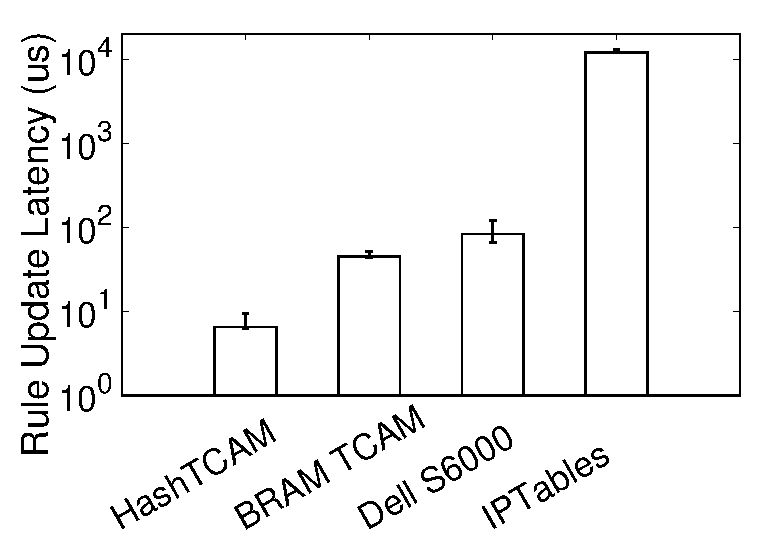
\includegraphics[width=0.45\textwidth]{eval/fw_5}
		}
		\vspace{-10pt}
		\caption{Firewalls. Error bars represents the $5^{th}$ and $95^{th}$ percentile. (a) and (b) Packet size is 64B.}
		\vspace{-10pt}
		\label{fig:firewall}
	\end{minipage}
	\begin{minipage}{.3\textwidth}
		\centering
		\subfigure[]{
			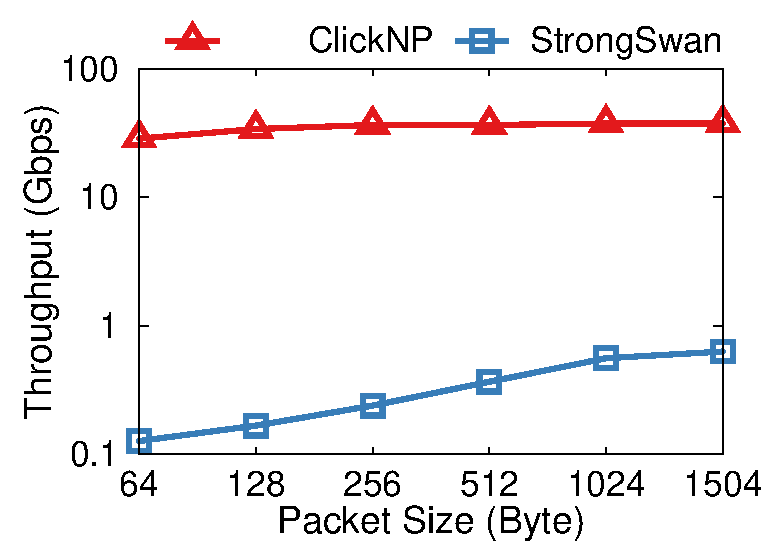
\includegraphics[width=0.9\textwidth]{eval/ipsec_1}
		}
		\subfigure[]{
			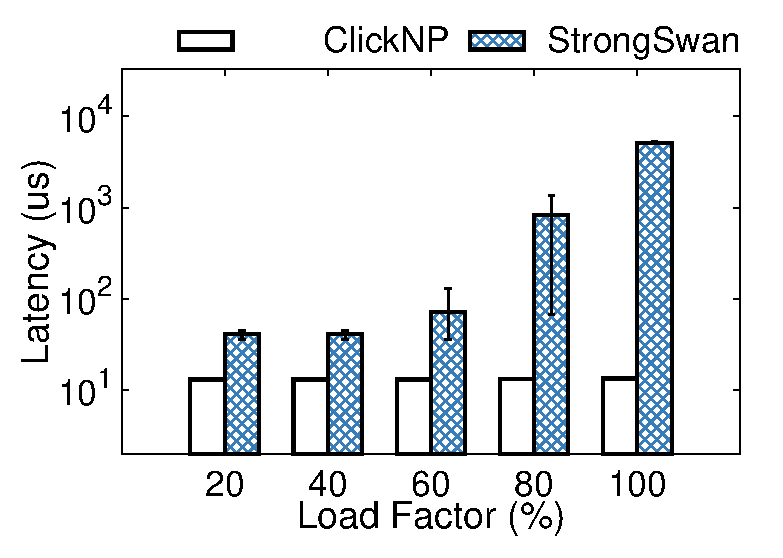
\includegraphics[width=0.9\textwidth]{eval/ipsec_2}
		}
		\vspace{-10pt}
		\caption{IPSec gateway. }
		\vspace{-10pt}
		\label{fig:IPSec}
	\end{minipage}
\end{figure*}

\subsection{Throughput and latency}

%In this subsection, we benchmark the throughput and latency of \name\ NFs.

\smalltitle{OpenFlow firewall.} 
In this experiment, we compare OFW with Linux firewall as well as Click+DPDK~\cite{barbette2015fast}.
For Linux, we use IPSet to handle exact-match rules, while use IPTables for wildcard rules.
As a reference, we also include the performance of Dell S6000 switch, which has limited firewall capability 
and supports 1.7K wild-card rules.
It is worth noting that the original Click+DPDK~\cite{barbette2015fast} does not support Receive Side Scaling(RSS).
In this work, we have fixed this issue and find when using 4 cores, Click+DPDK already achieves the best performance. 
But for Linux, we use as many cores as possible (up to 8 due to RSS limitation) for best performance. 

Figure~\ref{fig:firewall}(a) shows packet processing rates of different firewalls with different number of wild-card rules.
The packet size is 64B.
We can see that both \name\ and S6000 can achieve a maximum speed of 56.4~Mpps. 
Click+DPDK can achieve about 18~Mpps. 
Since Click uses a static classification tree to implement wildcard-match, the processing speed 
does not change with the number of rules inserted. 
%
Linux IPTables has a low processing speed of 2.67~Mpps, and the speed decreases as the number of rules
increases. This is because IPTables performs linear matching for wild-card rules.

Figure~\ref{fig:firewall}(b) shows the processing latency under different loads with small packets (64B) and 8K rules. 
Since each firewall has significantly different capacity, the load factor is normalized to the maximum processing speed of each system. 
%
Under all levels of load, FPGA (\name) and ASIC (S6000) solutions have $\mu$s-scale latency (1.23$\mu$s for ClickNP and 0.62$\mu$s for S6000) with very low variance (1.26$\mu$s for ClickNP and 0.63$\mu$s for S6000 at 95\% percentile).
However, the software solutions have much larger delay, and also much larger variance. 
For example, with Click+DPDK, when the load is high, the latency can be as high as $50\mu s$.
%
Figure~\ref{fig:firewall}(c) shows the processing latency with different packet sizes and 8K rules.
With software solutions, the latency increases with the packet size, mainly due to the larger 
memory to be copied.
In contrast, FPGA and ASIC retain the same latency irrespective to the packet size. 
In all experiments, the CPU usage of \name\ OFW is very low ($<5\%$ of a core).

Finally, Figure~\ref{fig:firewall}(d) shows rule insertion latency when there are already 8K rules. Click's static classification tree requires a prior knowledge of all rules, and generating tree for 8K rules takes one minute.
IPTables rule insertion takes 12ms, which is proportional to the number of existing rules in the table.
Rule insertion in Dell S6000 takes 83.7$\mu$s.
For \name, inserting a rule into HashTCAM table takes 6.3\approx9.5$\mu$s for 2\approx3 PCIe round-trips, while SRAM TCAM table takes 44.9$\mu$s on average to update 13 lookup tables.
\name\ data plane throughput does not degrade during rule insertion.
We conclude that OFW has similar performance as ASIC in packet processing, but is flexible and reconfigurable.



\smalltitle{IPSec gateway.} We compare IPSecGW with StrongSwan~\cite{strongswan}, using the same cipher suite of
AES-256-CTR and SHA1. We setup one IPSec tunnel and Figure~\ref{fig:IPSec}(a) shows the throughput with different packet sizes.
With all sizes, IPSecGW achieves line rates, \ie, 28.8Gbps with 64B packets and 37.8 Gbps with 1500B packets. 
%
StrongSwan, however, achieves only a maximum of 628Mbps, and the throughput decreases as packets become smaller.
This is because with smaller size, the number of packets needed to be processed increases, 
and therefore the system needs to compute more SHA1 signatures.
%
Figure~\ref{fig:IPSec}(b) shows the latency under different load factors. Again, IPSecGW yields constant latency of 13$\mu$s, 
but StrongSwan incurs larger latency with higher variance, up to 5ms!

\begin{figure*}[t!]
	\centering
	
	\subfigure[]{
		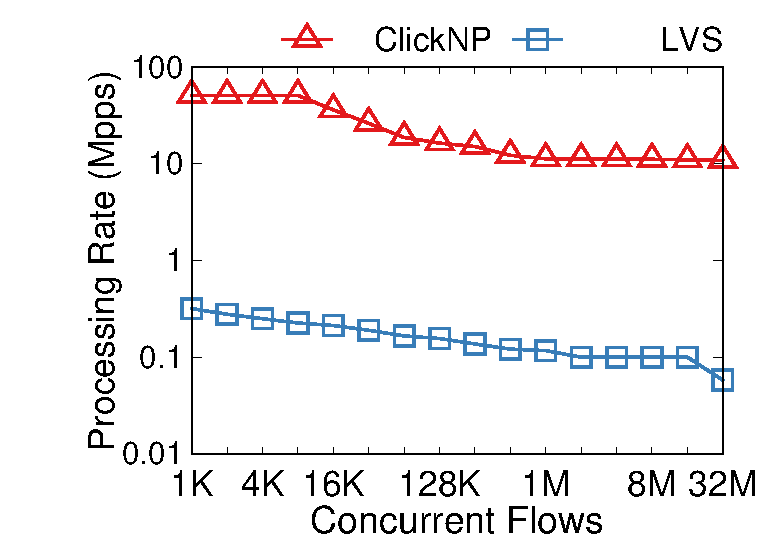
\includegraphics[width=0.3\textwidth,height=0.21\textwidth]{eval/l4_2}
	}
	\subfigure[]{
		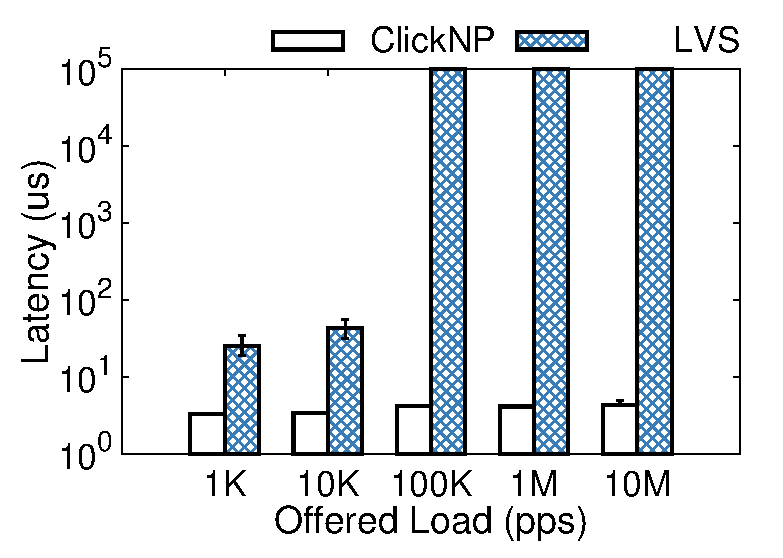
\includegraphics[width=0.3\textwidth]{eval/l4_1}
	}
	\subfigure[]{
		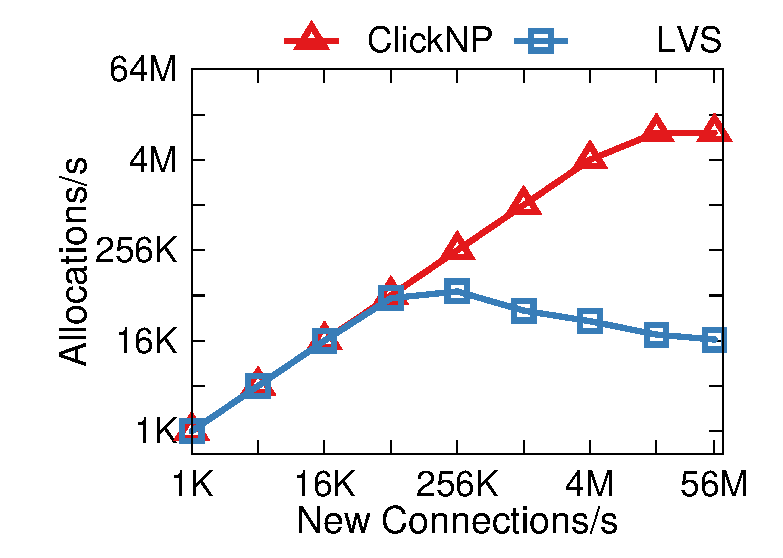
\includegraphics[width=0.3\textwidth]{eval/l4_3}
	}
\vspace{-10pt}
	\caption{L4 Load Balancer.}
	\label{fig:l4}
\vspace{-10pt}
\end{figure*}


\smalltitle{L4 load balancer.} We compare L4LB with Linux Virtual Server (LVS)~\cite{lvs}.
To stress test the system, we generate a large number of concurrent UDP flows with 64B packets, targeting one virtual IP (VIP).
Figure~\ref{fig:l4}(a) shows the processing rates with different number of concurrent flows.
When the number of concurrent flows is less than 8K, L4LB achieves the line rate of 51.2Mpps.
However, when the number of concurrent flows becomes larger, the processing rate starts to drop.
This is because of flow cache misses in L4LB. 
When a flow is missing in the flow cache,  L4LB has to access the onboard DDR memory,
which results in lower performance.
When there are too many flows, \eg, 32M, cache miss dominates and for most of the packets, 
L4LB needs to have one access to the DDR memory. So the processing rate reduces to 11Mpps.
In any case, the processing rate of LVS is low.  
Since LVS associates a VIP to only one CPU core, its processing rate is bound to 200Kpps.

Figure~\ref{fig:l4}(b) shows the latency under different load conditions. 
In this experiment, we fix the number of concurrent flows to 1 million. 
We can see that L4LB achieves very low latency of $4\mu$s.
LVS, however, incurs around $50\mu$s delay.
This delay goes up quickly when the offered load is higher than 100Kpps, which exceeds the  capacity of LVS. 

Finally, Figure~\ref{fig:l4}(c) compares the capability of L4LB and LVS to accept new flows. 
In this experiment, we instruct PktGen to generate as many one-packet tiny flows as possible.
We can see that L4LB can accept up to 10M new flows per second.
%
Since a single PCIe slot can transfer 16.5M flits per second, the bottleneck is still DDR access.
%
Our \textit{DIPAlloc} element simply allocates DIP in a round-robin manner.
For complex allocation algorithms, the CPU core of \textit{DIPAlloc} will be the bottleneck, and the performance can be improved by duplicating \textit{DIPAlloc} elements on more CPU cores.
For LVS, due to the limited packet processing capacity, it can only accept up to 75K new flows per second.

\egg{
\textbf{Stateful L4 load balancer.} We compare our ClickNP implementation with Linux Virtual Server (LVS) \cite{lvs} using both real-world traffic trace on a L4 load balancer \cite{gandhi2014duet} and synthetic traces to simulate adversary scenarios.
The real-world trace contains 1.3M flows collected in two hours with 26Gbps average throughput and 45KB median flow size.
The first adversary trace is round-robin scheduling packets from a large number of infinite UDP flows with 64B packet size to stress the load balancer under high concurrency.
The second adversary trace is a lot of tiny UDP flows to test how many new connections the load balancer can process per second.

Figure \ref{fig:l4} shows that ClickNP L4 load balancer has 50\approx500x lower latency than LVS on real-world trace, supports 32M concurrent flows and able to accept \approx10M new flows per second.
This performance is comparable to high-end hardware load balancers \cite{f5loadbalance}, while ours have low cost and high flexibility.
Figure \ref{fig:l4} also shows the importance of SRAM cache and pipelined DRAM access.
Our board can perform at most 13.6M DRAM random reads per second, and our new flow allocation rate gets near this limit thanks to pipelined DRAM access.
}

\egg{
First we test the performance under real-world data center traffic. We adopted the same traffic trace as DUET\cite{}, and picked the first ten minutes as testing data. Figure \ref{fig:l4} shows the four experiments we performed on the L4 load balancer. We first use TCP traffic to evaluate the flow completion time (FCT) under different throughputs. Then we use UDP traffic to evaluate the latency. 

Next we tested the performance with adversary traffic to thest the worst case performance. We fixed every flow to be one 1504 byte packet, and test the throughput under different flow numbers, and latency under different new flow rates.
}

\subsection{Resource utilization}

In this subsection, we evaluate the resource utilization of \name\ NFs.
Table~\ref{tab:applications} summarizes the results. 
Except for IPSec gateway which uses most BRAMs to hold coding books, 
all other NFs only use moderate resources (5\approx 50\%).  
There is still room to accommodate even more complex NFs.

Next, we study the overhead of fine-grained modularization of \name. 
Since every element will generate a logic block boundary and use only FIFO buffers to communicate with other blocks,
there should be an overhead.
To measure this overhead, we create a simple element that only passes data from one input port to an output port.
The resource utilization of this \textit{empty} element should well capture the overhead of modularization.
Different HLS tools may use different amount of resources, but all are low, with a min of 0.15\% to a max of 0.4\%.
So we conclude \name\ incurs little overhead due to modularization.

Finally, we want to study the efficiency of RTL code generated by \name, compared to hand-written HDL. 
To do so, we use NetFPGA~\cite{netfpga} as our reference.
We extract the key modules in NetFPGA, which are well optimized by experienced Verilog programmers, 
and implement counterpart elements in \name\ with the same functionality. 
We compare the relative area cost between these two implementations using different HLS tools as a backend.
The results are summarized in Table~\ref{tab:netfpga}.
Since different tools may have different area costs, we record both the maximum and minimal value.
%
We can see generally, automatically generated HDL code uses more area compared to hand-optimized code.
The difference, however, is not very large. 
For complex modules (shown in the top part of the table), the relative area cost is less than 2x.
%
For tiny modules (shown in the bottom part of the table), the relative area cost appears larger, but the absolute 
resource usage is small.
This is because all HLS tools
would generate a fixed overhead that dominates the area cost for tiny modules. 

In summary, \name\ can generate efficient RTL for FPGA that incurs only moderate area cost, 
which is capable of building practical NFs.
Looking forward, FPGA technology is still evolving very rapidly. For example, the next
generation FPGA from Altera, Arria 10, would have 2.5x more capacity than the chip we use
currently. 
Therefore, we believe the area cost of HLS would be less of a concern in the future. 

\vspace{10pt}


\egg{
Figure \ref{tab:applications} shows Logic Elements (LE) and BRAM footprint of aforementioned ClickNP applications.
Catapult shell and OpenCL runtime take 30\% LEs and 18\% BRAMs in addition to ClickNP applications.
}

\begin{table}[t!]
	\centering
	\vspace{-5pt}
	\caption{Summary of ClickNP NFs.}
	\label{tab:applications}
	\scalebox{0.9}{
		\begin{tabular}{l|r|r|r|r}
			\toprule
			Network Function & LoC$^\dagger$ & \#Elements & LE & BRAM \\
			\midrule
			\egg{
			Pkt generator & 13 & 6 & 16\% & 12\% \\
			Pkt capture & 12 & 10 & 8\% & 5\% \\
			OpenFlow firewall & 23 & 7 & 32\% & 54\% \\
			IPSec gateway & 37 & 10 & 35\% & 74\% \\
			L4 load balancer & 42 & 13 & 36\% & 38\% \\
			pFabric scheduler & 23 & 7 & 11\% & 15\% \\
			}
			Pkt generator & 665 & 6 & 16\% & 12\% \\
			Pkt capture & 250 & 11 & 8\% & 5\% \\
			OpenFlow firewall & 538 & 7 & 32\% & 54\% \\
			IPSec gateway & 695 & 10 & 35\% & 74\% \\
			L4 load balancer & 860 & 13 & 36\% & 38\% \\
			pFabric scheduler & 584 & 7 & 11\% & 15\% \\
			\bottomrule
			\multicolumn{5}{l}{$^\dagger$ Total line of code of all element declarations and} \\
			\multicolumn{5}{l}{configuration files.}
		\end{tabular}
	}
\vspace{-10pt}
\end{table}

\egg{
To evaluate ClickNP's area cost overhead compared to hand-written HDL, we implemented several ClickNP elements resembling network functions in NetFPGA 10G \cite{netfpga} reference router and Openflow switch projects.
Table \ref{tab:netfpga} compares ClickNP's relative area cost over NetFPGA using Vivado HLS 2015.4 and Altera OpenCL 15.1.
Most ClickNP implementations show less than 100\% logic overhead and less than 30\% BRAM overhead. For tiny elements (\eg IP checksum), a fixed element overhead dominates.
}

\begin{table}[t!]
	\centering
	\vspace{-5pt}
	\caption{Relative area cost compared to NetFPGA.}
	\label{tab:netfpga}
	\scalebox{0.9}{
		\begin{tabular}{l|r|r|r}
			\toprule
			\multirow{2}{2.2cm}{NetFPGA Function} & LUTs & Registers & BRAMs \\
						& Min / Max & Min / Max & Min / Max \\
			\midrule
			Input arbiter  & 2.1x / 3.4x & 1.8x / 2.8x & 0.9x / 1.3x \\
			Output queue   & 1.4x / 2.0x & 2.0x / 3.2x & 0.9x / 1.2x \\
			Header parser  & 0.9x / 3.2x & 2.1x / 3.2x & N/A \\
			Openflow table & 0.9x / 1.6x & 1.6x / 2.3x & 1.1x / 1.2x \\
			\midrule
			\midrule
			IP checksum    & 4.3x / 12.1x & 9.7x / 32.5x & N/A \\
			Encap          & 0.9x / 5.2x & 1.1x / 10.3x & N/A \\
			\bottomrule
		\end{tabular}
	}
\vspace{-10pt}
\end{table}

\egg{
Original data:
Function	LUTs			Registers			BRAMs		
NetFPGA	AOCL	VHLS	NetFPGA	AOCL	VHLS	NetFPGA	AOCL	VHLS
Input arbiter	2048	4346	6998	4553	12843	8348	30	40	26
Output queue	3824	5280	7542	6479	13409	21005	22.5	26	20
Header parser	626	2012	567	698	6095	817	N/A		
Openflow table	3923	6322	3535	4438	10171	7140	33.5	40	38
IP checksum	207	2511	884	162	5269	1576	N/A		
Encap	684	3536	636	821	8493	871	N/A	
}

\subsection{Validation of pFabric}
Before we end this section, we show that \name\ is also a good tool for network research.
Thanks to the flexibility and high performance, we can quickly prototype the latest research 
and apply it to real environments.
For example, we can easily implement pFabric scheduler~\cite{pfabric} using \name, and 
apply it in our testbed.
%
In this experiment, we modify a software TCP flow generator~\cite{mqecn} to place the flow
priority, \ie, the total size of the flow, in packet payload.
We generate flows according to the data-mining workload in~\cite{pfabric} and further
the restrict egress port to be 10~Gbps using a \textit{RateLimit} element.
We apply pFabric to schedule flows in egress buffer according to flow priorities. 
Figure~\ref{fig:pfabric} shows the average flow completion time (FCT) of pFabric, TCP with Droptail queue, and the ideal.
This experiment validates that pFabric achieves near ideal FCT in this simple scenario.

\begin{figure}[h!]
\centering
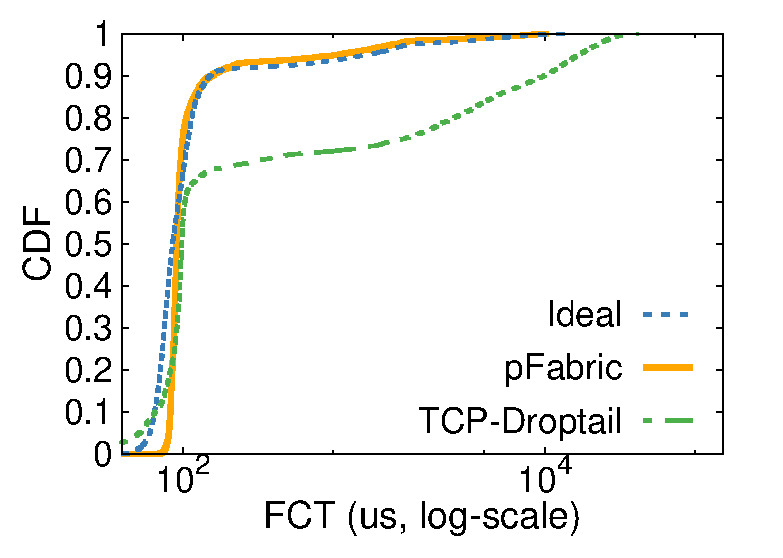
\includegraphics[width=0.3\textwidth]{eval/pfabric}
\vspace{-10pt}
\caption{Validation of pFabric.}
\label{fig:pfabric}
\vspace{-10pt}
\end{figure}


\egg{
\subsection{Network Benchmark Suite}

\subsubsection{Configurable Flow Generator}

\begin{lstlisting}
Rand(0,1,2) -> MetaGen(1,1) -> RevParser(1,1) -> IPChecksum(1,1) -> TCPChecksum(1,1) -> NVGRE_Encap(1,1) -> tor_out
\end{lstlisting}

\subsubsection{Packet Trace Replay}

\begin{figure}[h!]
	\centering
	
\includegraphics[width=0.6\columnwidth]{image/logo}
	\vspace{-0.15in}
	\caption{Traffic Replay Throughput, x: packet size, y: Gbps, lines: ClickNP, CPU}
	\vspace{-0.15in}
	\label{fig:TrafficReplayPerformance}
	%    \vspace{-2mm}
\end{figure}

\subsubsection{Traffic Monitor}

\begin{lstlisting}
tor_in -> Receiver -> Drop (1,0)
\end{lstlisting}

latency, throughput, sequence number check

\subsection{Network Virtualization}

\subsubsection{NVGRE Tunneling}

\begin{figure}[h!]
	\centering
	
\includegraphics[width=0.6\columnwidth]{image/logo}
	\vspace{-0.15in}
	\caption{Tunnel Encap + Decap Performance, x: packet size, y: Gbps, lines: ClickNP, Hyper-V}
	\vspace{-0.15in}
	\label{fig:NVGREPerformance}
	%    \vspace{-2mm}
\end{figure}

\subsubsection{Per-VM Metering and Rate Limiting}

\subsection{Security}

\subsubsection{Network-layer Firewall}

\begin{lstlisting}
Parser :: parser(1,2)
DropPolicer :: action(2,2)
tor_in -> parser[1] -> [1]action[1] -> nic_out
parser[2] -> ExtractFiveTuple(1,1) -> Hashtable @(1,1) -> [2]action[2] -> Drop (1,0)
\end{lstlisting}

\begin{figure}[h!]
	\centering
	
\includegraphics[width=0.6\columnwidth]{image/logo}
	\vspace{-0.15in}
	\caption{Network-layer Firewall Performance, x: \#rules, y: pps, lines: ClickNP, Linux iptables}
	\vspace{-0.15in}
	\label{fig:FirewallPerformance}
	%    \vspace{-2mm}
\end{figure}

\subsubsection{Application-layer Firewall}

\begin{lstlisting}
Parser :: parser(1,2)
DropPolicer :: action(2,2)
tor_in -> parser[1] -> [1]action[1] -> nic_out
parser[2] -> ExtractFiveTuple(1,1) -> RegexMatch @(1,1) -> [2]action[2] -> Drop (1,0)
\end{lstlisting}

\begin{figure}[h!]
	\centering
	
\includegraphics[width=0.6\columnwidth]{image/logo}
	\vspace{-0.15in}
	\caption{Application-layer Firewall Performance, x: \#rules, y: Gbps, lines: ClickNP, snort \cite{roesch1999snort}}
	\vspace{-0.15in}
	\label{fig:WAF_Performance}
	%    \vspace{-2mm}
\end{figure}

\subsubsection{DDoS Detection with Bitmap Sketch}

\begin{lstlisting}
Parser :: parser(1,2)
tor_in -> parser[1] -> nic_out
parser[2] -> ExtractVMID(1,1) -> HashTable @(1,1) -> ExtractSrcIP(1,1) -> BitmapSketch @(1,1) -> Drop (1,0)
\end{lstlisting}

OpenSketch \cite{yu2013software}

\begin{figure}[h!]
	\centering
	
\includegraphics[width=0.6\columnwidth]{image/logo}
	\vspace{-0.15in}
	\caption{Sketch Accuracy, x: \#real flows, y: relative error (\%) with error bar}
	\vspace{-0.15in}
	\label{fig:SketchAccuracy}
	%    \vspace{-2mm}
\end{figure}


\subsection{Scheduling}

\subsubsection{PIAS Tagging}

PIAS \cite{bai2014pias}

\subsubsection{Generic Priority Queue}

pFabric \cite{alizadeh2013pfabric}

\subsubsection{Packet Pacing}

Silo \cite{jang2015silo}

\begin{figure}[h!]
	\centering
	
\includegraphics[width=0.6\columnwidth]{image/logo}
	\vspace{-0.15in}
	\caption{CDF of pacing inaccuracy due to buffer overflow, x: percentile, y: time shift, lines: buffer sizes}
	\vspace{-0.15in}
	\label{fig:PacingAccuracy}
	%    \vspace{-2mm}
\end{figure}

\subsubsection{Timestamping}

TIMELY \cite{mittal2015timely} measures RTT as the signal for congestion control. It requires both receive and send timestamping feature and hardware-generated ACK of recent NICs. Furthermore, since ACKs have already been sent by NIC hardware, OS networking stack needs modifications to avoid generating duplicate ACKs.

With ClickNP we can do the same latency measurement without using a NIC with timestamping feature, and does not require modification to the OS networking stack, as long as the FPGAs at sender and receiver have same clock frequency. The idea is to subtract the latency spent in receiver-side OS networking stack. Upon reception of a data packet, we subtract the timestamp and expects the OS to echo back the timestamp in the ACK packet. When the ACK packet is sent, we add the timestamp, as if we had shifted the initial timestamp by OS processing latency. Pseudo code:

\begin{lstlisting}
.element SendTimestamp {
    .state { uint timestamp = 0; }
    .handler {
        if (input_ready) {
            if (!is_ack_packet())
                set_tsval (timestamp);
            else
                set_tsecr (get_tsecr() + timestamp);
        }
        timestamp ++;
    }
}
.element RecvTimestamp {
    .state { uint timestamp = 0; }
    .handler {
        if (input_ready) {
            if (!is_ack_packet())
                set_tsval (get_tsval() - timestamp);
            else
                set_tsval (timestamp);
        }
    }
}
nic_in -> Parser (1,2) -> SendTimestamp (2,1) -> tor_out
tor_in -> Parser (1,2) -> RecvTimestamp (2,1) -> nic_out
\end{lstlisting}

\begin{figure}[h!]
	\centering
	
\includegraphics[width=0.6\columnwidth]{image/logo}
	\vspace{-0.15in}
	\caption{CDF of measured RTT, x: percentile, y: RTT, lines: hardware ACK (ideal), remove OS latency (close to ideal), not remove OS latency (poor)}
	\vspace{-0.15in}
	\label{fig:TimestampAccuracy}
	%    \vspace{-2mm}
\end{figure}
}

\egg{
Figure~\ref{fig:trafficgen} shows the throughput of \name\ traffic generator and capture. We can see that the generator can
generate packets at line-rate of 40 Gbps. 
When packet size is small ($<256B$), the measured throughput is slightly less than 40 Gbps. We confirm this is due to a
bug in Ethernet MAC in the shell, which may drop a few flits when packet rate is high. 
Figure~\ref{fig:trafficgen}(b) shows the capture performance in packet per second.  

\begin{figure}[t!]
	\centering
	\subfigure[] {
	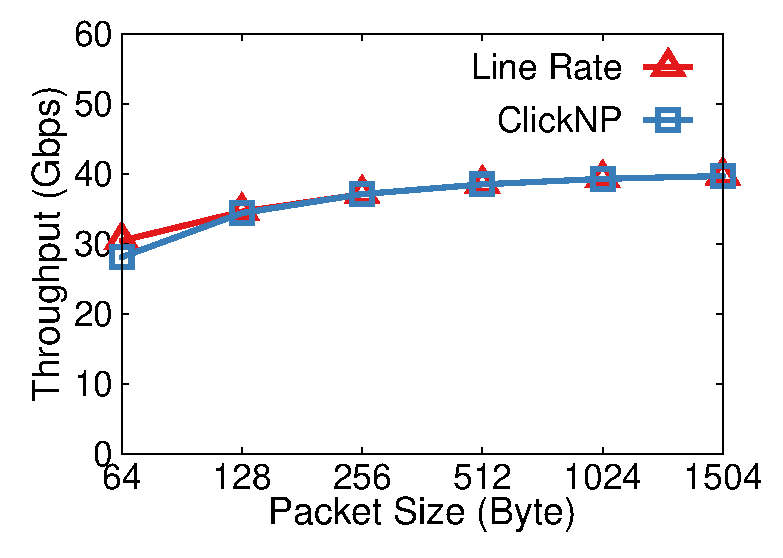
\includegraphics[width=0.225\textwidth]{eval/trafficgen}
	}
	\subfigure[] {
	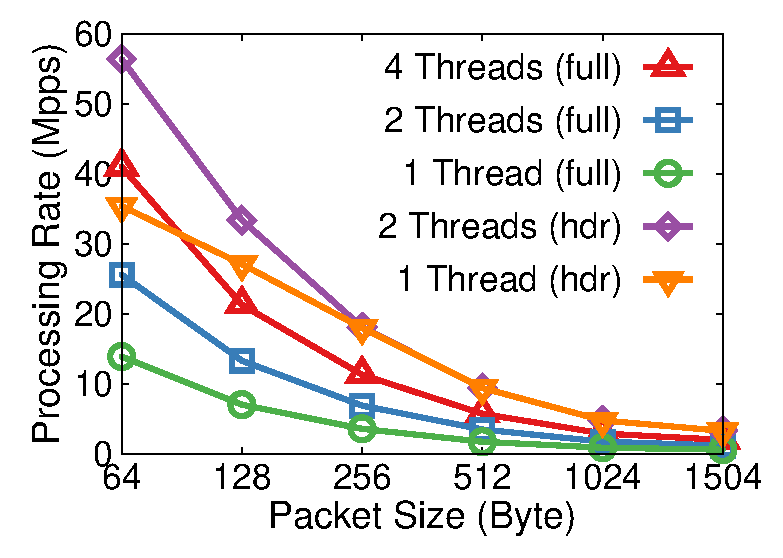
\includegraphics[width=0.225\textwidth]{eval/dump}
	}
	\vspace{-15pt}
	\caption{(a) Traffic generator. (b) Traffic capture.}
	\label{fig:trafficgen}
\end{figure}
}
\egg{
In this section we evaluate throughput and latency of applications presented in section \ref{sec:application}. All these application can achieve line-rate throughput and microsecond-scale latency for reasonable traffic patterns. Latency is averaged over $1000$ rounds, and error bars mark the $5\%$ and $95\%$ percentile.

\textbf{Traffic generator.} We use our traffic generator to send packets to NIC, and use Windows Performance Monitor to measure the throughput. As shown in Figure \ref{fig:trafficgen}, our generator is able to generate packets at 40Gbps line rate when the packet size is not less than 256 bytes. The small gap for 64-byte packets is due to lack of back-pressure in 40GbE MAC of FPGA shell.

\textbf{Traffic capture.} We evaluate the throughput of dumper and results are presented in \ref{fig:dump}.
Each host kernel runs on a separate core and traffic is split evenly to kernels by flow tuple hash.
With four host elements receiving the packets, we can approximately achieve the maximum speed of the PCIe channel.
When we only need the flow tuple and timestamp, ClickNP can easily capture line rate with two cores.
}

\egg{
\textbf{IPSec gateway.} We use StrongSwan \cite{strongswan} with AES256CTR + SHA1 IKEv2 cipher suite as baseline.
After setting up IPSec keys and nonces in ClickNP elements via signal, we send UDP packets in a single IPSec tunnel to test throughput and latency on encryption path.
StrongSwan leverages only one CPU core due to tunnel message sequencing.
As shown in Figure \ref{fig:IPSec}, \textit{Reservo} to exploit packet-level parallelism for SHA-1 element shows 40x performance gain compared to unoptimized version. }

\egg{
\textbf{OpenFlow firewall.} We compare our firewall with Click + DPDK \cite{barbette2015fast} on 4 cores, and Linux iptables (for wildcard match) / ipset \cite{ipset} (for exact match) with RSS on 8 cores.
We also include Dell S6000, a high-end commodity switch, as a reference.

We optimized FromDPDKDevice element in Click to enable receiving packets on multiple cores, while the bottleneck becomes Mellanox polling-mode driver at 18 Mpps.
Click uses a radix tree for exact IP lookup and a classification tree for wildcard flow tuple lookup, so table lookup is not bottleneck of Click.
Linux ipset uses hash table for exact lookup. Linux iptables match wildcard rules linearly, which is the source of low throughput and high latency.
Dell S6000 supports 1.7K 5-tuple wildcard match rules.
For all packet sizes and number of rules, ClickNP offers line rate throughput and latency comparable to commodity ASIC.

Additionally, for 8K wildcard rules, Click takes minutes to generate the classification tree and cannot offer live rule update. ClickNP can perform 350K live rule updates per second while the data plane keeps line forwarding rate. Dell S6000 can perform 12K live rule updates per second.

16K exact, 8 K wild.
}

\egg{
All results are presented in Figure \ref{fig:firewall}. The first two subfigures are to show how packet size and rule numbers influence throughput. In the first subfigure, the packet size is fixed at 64 byte. And in the second subfigure, the numbers of rules is set to be 64k(exact)/8k(wild).

The last two subfigures are about latency. In \ref{}, we fixed the packet size to be ?? and evaluated the latency with different loads. In \ref{}, we change the packet size to see how the latency changes in maximum load scenario. 

From all these figures we can see that ClickNP approximates the performance of Dell S6000, and has a ???x boost on the CPU solution.
}

%!TEX root=main.tex

\section{Related Work}
\label{sec:related}

% software network functions
Software NFs have great flexibility and scalability.
% Software switches 
Early studies mainly focus on software-based packet forwarding~\cite{routebricks, Egi:2008:THP:1544012.1544032 }. 
They show that multi-core x86 CPU can forward packets at near 10Gbps per server
and the capacity can scale by clustering more servers. 
%
Recently, many  systems have been designed to implement various types of NFs~\cite{comb, Greenhalgh:2009:FPR:1517480.1517484, martins2014clickos}. 
Similarly, all of these systems exploit the multi-core parallelism in CPUs to achieve close to 10Gbps 
throughput per machine, and scale out to use more machines when higher capacity is needed. 
%
Ananta~\cite{ananta} is a software load-balancer deployed in Microsoft datacenters to provide 
cloud-scale load-balancing service.
%
While software NFs can scale out to provide more capacity, doing so adds 
considerable costs in both CAPEX and OPEX~\cite{ananta, duet}.

% accelerations
To accelerate software packet processing, previous work has proposed using GPU~\cite{packetshader},
specialized network processor (NP)~\cite{cavium,netronome }, and hardware switches~\cite{duet}.
% GPU
GPU is primarily designed for graphic processing and recently extended to other applications with massive 
data parallelism. GPU is more suitable for batch operations. Han, \etal~\cite{packetshader}, show that using GPU
can achieve 40Gbps packet switching speed. 
However, batch operations incur high delay. 
For example, the forwarding latency reported in \cite{packetshader} is about $200\mu s$, two orders of 
magnitude larger than \name.
Compared to GPU, FPGA is more flexible and can be reconfigured to capture data and pipeline parallelisms, both of which are very common in NFs.
% NP
NPs, however, are specialized to handle network traffic and have many hard-wired network accelerators.
In contrast, FPGA is a general computing platform. 
Beside NFs, FPGA have many other applications in datacenters, making it more attractive 
to deploy at scale~\cite{putnam2014reconfigurable}.
%
Hardware switch has limited functionality and its applications are very restricted~\cite{duet}.

FPGA is a mature technology and recently has been deployed to accelerate datacenter services, including NFs~\cite{putnam2014reconfigurable, smartnic, rubow2010chimpp, lavasani2012compiling}.
It is well recognized that the programmability of FPGA is low and there is a 
rich body of literature on improving it, 
by providing high-level programming abstractions~\cite{bluespec, auerbach2010lime, bacon2013fpga, singh2011implementing, bachrach2012chisel, wester2015transformation}.
%
Gorilla \cite{lavasani2012compiling} proposes a domain-specific high-level language for packet switching on FPGA.
Chimpp \cite{rubow2010chimpp}, however, tries to introduce Click model into HDL 
to develop modular router.
\name\ works along this direction and is complimentary to previous work.
\name\ targets NFs in datacenters, and addresses the programmability issue by
providing a highly flexible, modularized architecture and leveraging commercial HLS tools.

% add comments on rubow2010chimpp,
The work most related to ours is the Click2FPGA toolchain~\cite{Click2NetFPGA}, which compiles an entire Click configuration to FPGA. 
Its performance, however, is much lower than \name\ and it lacks support for 
joint CPU/FPGA packet processing.
\egg{
High performance PCIe communication designs between CPU and co-processors are explored in~\cite{lee2015flosis, nam2015haetae}. 
ClickNP follows this line of work and proposes a design for efficient joint CPU-FPGA processing.}
%
To the best of our knowledge, \name\ is the first FPGA-accelerated platform for general NFs
processing at 40Gbps line rate, and completely written in high-level language.

%%!TEX root=main.tex
\section{Future Work}
\label{sec:future}

One challenge for deploying ClickNP in production data centers is 30-second interruption of data plane while FPGA is being reprogrammed. Partial reconfiguration \cite{bourgeault2011alteras} feature of FPGA can be utilized to keep basic packet forwarding functionality while FPGA is being reprogrammed.

On-chip DRAM has relatively low throughput which is insufficient for rule caching and line-rate packet buffering. The problem can be mitigated if host memory can be utilized by kernels. Using existing PCIe streaming interface to access host DRAM incurs high CPU overhead and high latency. In theory the FPGA should be able to access host DRAM via DMA directly, but the implementation of a random-access DMA engine is left for future work.

OpenCL does not provide a way for explicit pipeline control. We cannot control when and where a large combinational logic is split to pipeline stages. Say we have a data handler which loads from a block SRAM, performs a multiplication operation that takes 3 cycles, then stores the result back to it. The OpenCL scheduler will launch the iteration every 3 cycles due to memory dependency. A hardware developer, however, could pipeline the iteration by running three multiplication logics in parallel and re-issuing operations with conflicting addresses -- a well-known technique in superscalar processor and speculative execution.

OpenCL also does not allow explicit specification of an array to be registers or block SRAM. When we need to use a variable to index an array while keeping it as registers instead of block SRAM, we have to use \textit{.repeat} statement to duplicate many copies of a code snippet.

Furthermore, OpenCL cannot figure out independently accessed memory regions and therefore split them into different memory banks. If we use a two-dimensional array \textit{value[DEPTH][WIDTH]} instead of one single-dimensional array \textit{valueN[WIDTH]} per stage in the \textit{IP\_Checksum} example, all accesses to the two-dimensional array would be considered dependent. A similar problem happen to struct members. A symbolic execution engine might be able to recognize such virtual memory dependencies and therefore split the array into distinct memory banks.

Although ClickNP provides abstractions and coding conventions for exploiting spatial and temporal parallelism, software developers still need to learn these abstractions and programming guidelines in order to write fully pipelined elements. Another approach might be recognizing some common coding styles for software programmers bearing the CPU model, and optimize the code automatically. This approach is achievable to some extent, for example, if a loop does not have constant terminating condition, we can still unroll it if the maximum possible iterations can be inferred.
%!TEX root=main.tex
\section{Conclusion}
\label{sec:conclusion}

% compile time?

This paper presents \name, an FPGA-accelerated platform for highly flexible 
and high-performance NFs in commodity servers.
\name\ is completely programmable using high-level language and provides a 
modular architecture familiar to software programmers in the networking field.
\name\ supports joint CPU/FPGA packet processing and has high performance.
Our evaluations show that \name\ improves the throughput of NFs by 10x compared to
state-of-the-art software NFs, while alos reducing latency by 10x.
%
Our work makes a concrete case showing FPGA is capable for accelerating NFs in datacenters.
Also, we demonstrate that high-level programming for FPGA is actually feasible and practical. 
%
One limitation of FPGA programming, however, is that the compilation time is rather long, \eg, 1\approx 2 hours, largely
due to HDL synthesis tools.
% cross platform
\name\ alleviates this pain with its cross-platform ability, and hopes most bugs 
could be detected by running elements on CPU.
However, in the long term, HDL synthesis tools should be optimized to greatly 
shorten their compilation time.




%!TEX root=main.tex
\vspace{-6pt}
\section*{Acknowledgements}

We would like to thank Andrew Putnam, Derek Chiou, and Doug Burger for all technical discussions.
We'd also like to thank the whole Catapult v-team at Microsoft for the Catapult Shell and support of OpenCL programming.
We thank Albert Greenberg and Dave Maltz for their support and suggestions on the project.
We thank Tong He for his contribution on ClickNP PCIe channel development.
Finally, we also thank our shepherd, KyoungSoo Park, and other anonymous reviewers for their valuable feedbacks and comments.


\balance
\bibliographystyle{abbrv}
{\small \bibliography{reference}}

\end{document}
